\documentclass{article}
%
\usepackage{apacite}
\usepackage{authblk}
\usepackage[utf8]{inputenc}
\usepackage{pdfpages}
\usepackage{enumitem}
\usepackage{tikz}
\usepackage{amsmath}
\usepackage{amssymb}
\usepackage{stmaryrd}
\usepackage{float}
\usepackage{subcaption}
\usepackage{rotating}
\usepackage{comment}
\usepackage{graphics}
\usepackage[nottoc,notlot,notlof]{tocbibind}

\providecommand{\corrauthor}[1]
{
  \small	
  \textbf{{Corresponding author:}} #1
}

\providecommand{\Dataavailabilitystatement}[1]
{
  \small	
  \textbf{{Data availability statement:}} #1
}

\begin{document}
%

\begin{titlepage}
\title{\textit{Most} quantifiers have \textit{many} meanings}


\author[a]{Sonia Ramotowska\footnote{Institut für Sprache und Information, Gebäude 23.21. Etage 04 Raum 75, Heinrich-Heine-Universität Düsseldorf, Universitätsstraße 1, 40225 Düsseldorf, Germany}}
\author[b]{Julia Haaf}
\author[c]{Leendert Van Maanen}
\author[a]{Jakub Szymanik}
\affil[a]{Institute for Logic, Language and Computation, University of Amsterdam, Spuistraat 134, 1012 VB Amsterdam, The Netherlands}
\affil[b]{Psychological Methods, University of Amsterdam, Nieuwe Achtergracht 129-B, 1018 WT Amsterdam, The Netherlands}
\affil[c]{Department of Experimental Psychology \& Helmholtz Institute, Utrecht University, Heidelberglaan 1, 3584 CS Utrecht, The Netherlands}
\date{}

%
\maketitle    % typeset the header of the contribution
\vspace{6cm}
\corrauthor{Correspondence concerning this article should be addressed to Sonia Ramotowska (sonia.ramotowska@hhu.de or s.ramotowska@uva.nl).}

\vspace{1cm}
\textbf{Data availability statement:} The data and analysis code is available at https://github.com/jstbcs/pling-quant.
\end{titlepage}

\vspace{1cm}
\textbf{Abstract}

Formal semantic theories of meaning assume that function words, such as natural language quantifiers, have a rigid meaning expressed by their truth conditions. In this study, we challenge this view by showing that there are systematic individual differences in semantic representations of quantifiers. We selected five natural language quantifiers (\textit{few}, \textit{fewer than half}, \textit{many}, \textit{more than half}, and \textit{most}) and collected binary truth value judgement data in an online quantifier verification experiment. Using a Bayesian three-parameter logistic regression model, we separated three sources of individual differences: truth condition, vagueness, and response error. The k-means clustering of the parameters of the model revealed three subgroups of participants with different semantic representations of quantifiers and a different organization of the mental line of quantifiers. This finding supports the view that logical words, like content words, are sensitive to individual differences, and hence it challenges the traditional view on meaning.
%We selected five natural language quantifiers (\textit{few}, \textit{fewer than half}, \textit{many}, \textit{more than half}, and \textit{most}), which we expected to differ in the model parameters. We collected response data in an online experiment and fitted a Bayesian three-parameter logistic regression model. 
%Moreover, we found asymmetry between positive and negative quantifiers in response error and vagueness. 

\vspace{1cm}
\textbf{Keywords}

Quantifiers; vagueness; meaning representations; Hierarchical Bayesian Model
%
%
%
\section{Introduction} 
Needless to say, humans differ in their cognitive abilities. Similar to other cognitive domains, individual differences are also present in natural language processing \cite{Kidd2018}. They have been studied extensively in many natural language categories, including gradable adjectives \cite{Verheyen2018TypicalityDimensionalAdjectives, Verheyen2018Subjectivityiheavy/i}, semantic categorizations of nouns \cite{Verheyen2013AAmbiguity, Verheyen2018Subjectivityiheavy/i, Verheyen2019RevealingInconsistencies}, probability terms \cite{Wallsten86, Mosteller1990, Schuster2019adaptationuncertaintyexpressions}, and presuppositions projection \cite{Sudo2012PresuppositionProjection}. In this paper, we investigate individual differences in natural language quantifier representations. Quantifiers, such as \textit{many}, \textit{few}, \textit{most}, \textit{some}, and \textit{at least 5}, are functional words used to express quantities. They have drawn the attention of researchers from different fields ranging from logic \cite{Barwise1981GeneralizedLanguage, Mostowski1957OnQuantifiers} to formal semantics \cite{Keenan2012HandbookLanguage, Szabolcsi2010Quantification} to cognitive science (\citeNP{Ramotowska2020MostDifferences}; see \citeNP{Szymanik2016QuantifiersPerspectives} for review). They have been studied mostly in the verification paradigm \cite<e.g.,>{Deschamps2015ThePerception., Hackl2009, Pietroski2009, Schlotterbeck2020RepresentationalEffect}, in which participants have to decide if a quantified sentence is true in a given context. While the studies of quantifiers are common, individual differences in their use have gained somewhat less attention in the literature. The dominant perspective on quantity words considers meaning representations to be rigid logical forms (e.g., \citeNP{Barwise1981GeneralizedLanguage}, see also \citeNP{Hackl2009} for discussion). A growing body of evidence \cite{Denic2020Are, Ramotowska2020MostDifferences, Talmina2017} questions this traditional view and calls for incorporating individual differences in the domain of quantifiers.

Individual differences in quantifiers may come from three different sources. The first source are differences in general cognitive abilities, e.g., working memory \cite{Just1992AMemory, Kidd2018} or executive functions \cite{Kidd2018}. For example, the accuracy and speed of verification of proportional quantifiers depend on working memory capacities \cite{Steinert-Threlkeld2015, Zajenkowski2013MOSTPerspective, Zajenkowski2014WorkingVerification} and cognitive control \cite{Zajenkowski2013MOSTPerspective, Zajenkowski2014WorkingVerification}. The second source of individual differences could lie in the choice of verification strategies \cite{Talmina2017}. For example, \citeA{Talmina2017} showed that some participants prefer to use a precise strategy while verifying \textit{most}, and others choose an approximate strategy. Moreover, strategy preference depends on the context \cite{Register2018SemanticContext}. Finally, the third source of individual differences could be different meaning representations of quantifiers where individuals assign different truth values to the same sentence \cite{Spychalska2016InvestigatingPotentials}. \citeA{Spychalska2016InvestigatingPotentials} divided participants into two groups based on their truth value evaluation of the underinformative sentence ``\textit{Some} As are B" when in fact \textit{all} As were B. The group of so-called pragmatic responders judged the underinformative sentence as false and logical responders as true. 

While the first two sources of individual differences are compatible with the formal semantics perspective on language, the last one is a conundrum for linguistic tradition. At first glance, it seems that rational subjects cannot assign different truth conditions to logical words such as quantifiers. Moreover, the alignment of meanings between speakers is a crucial requirement for successful communication. \citeA{Douven2019naturalconcepts} referred to this principle as to \textit{correlation of meanings}. This requirement puts constraints on how much meaning of the single word can vary across speakers. 

To summarise, on the one hand, we have evidence from many different linguistic domains \cite{Verheyen2018TypicalityDimensionalAdjectives, Verheyen2018Subjectivityiheavy/i, Verheyen2013AAmbiguity, Verheyen2018Subjectivityiheavy/i, Verheyen2019RevealingInconsistencies, Wallsten86, Mosteller1990, Schuster2019adaptationuncertaintyexpressions, Sudo2012PresuppositionProjection} for between-participants variability in meaning representations. On the other hand, we have a constraint on variation in meanings that arises from the communication pressure. In this paper, we show that individual differences in quantifier representations are tangible. We aim to answer three questions regarding individual differences. First, we tested the ranges of variability in meaning representations of quantifiers. We argue that even though there is individual variation meaning representations, this variation is constrained. Previous studies \cite{Sudo2012PresuppositionProjection, Spychalska2016InvestigatingPotentials} showed that participants can form subgroups with different meanings. We propose to investigate the subgroups that would align the meaning of a quantifier within-group but have different meanings between groups. We will test \textit{how many subgroups of participants with different meanings we can identify}. 

Second, quantifiers convey information about quantities, and therefore they could be ordered with respect to the indicated amount on a mental line \cite<e.g.,>{Hammerton1976HowPart, Pezzelle2018}. \textit{None} is a lower bound on a mental line and expresses quantity of zero and \textit{all} is an upper bound that expresses quantity of 100\%. \textit{Few} is intuitively more than \textit{none} and less than \textit{many}, while \textit{many} could be less than \textit{all}. The variability in meanings between participants poses a question on \textit{how the meanings of quantifiers are interrelated at the subject level}. Given the correlation of meanings principle \cite{Douven2019naturalconcepts}, we hypothesize that participants should share the meanings of quantifiers at least to a certain extent. While they can choose various positions of a quantifier on a mental line, their choice for one quantifier constraints their choices for other quantifiers \cite{Heim2015Ifmany}. In this paper, we will test \textit{whether the order of quantifiers on the mental line is consistent among participants}. 

Third, we want to separate potential sources of individual variation in quantifier representations from variability in task performance. For example, we considered that participants may assign different truth conditions to the same quantifier. However, they can also make mistakes while performing the task (e.g., due to attentional lapses) that are unrelated to meaning representation. The third question regarding individual differences is, therefore: \textit{How can we separate the source of individual differences related to quantifier representation from variability in task performance}?

To answer these questions, we analyzed data from a quantifier verification task, in which participants were asked to judge the truth of a quantified sentence based on information about proportion. We modeled the choices using a logistic regression model to separate the individual differences meaning representations from variability in performance of the verification task. Then, we clustered participants based on their truth conditional representations to establish subgroups with aligned meanings. Our work continues the tradition of using computational modeling to better understand cognitive representations.
Computational modeling has previously been successfully applied to test competing semantic theories \cite<e.g.,>{vanTiel2021ProbabilisticQuantification} and to distinguish between different sources of individual differences in language processing \cite{Vasishth2019ComputationalProcessing, Waldon2020ModelingExperiments}. Moreover, computational modeling allows the investigation of qualitatively different effects in experimental data \cite{Haaf2019SomeStructures, DonzallazCreativeProcess, Kolvoort2021VariabilityJudgments, Miletic2019CautionAbility, Ramotowskathesis}. In the following section, we explain how we operationalized the meaning representations of quantifiers on model parameters.

%\subsection{How many subgroups of participants with different meanings can we identify?}
\subsection{Individual differences in truth conditional quantifier representations}
%The logical theory of meaning 
Traditionally, formal semantics analyses the meaning of quantifiers in terms of truth conditions (e.g., Generalized Quantifier Theory, \citeNP{Barwise1981GeneralizedLanguage, Mostowski1957OnQuantifiers}). The truth condition of a natural language quantifier specifies a threshold above or below which the quantifier is true\footnote{In this paper, we focus only on quantifiers with one threshold. Some quantifiers can have two or more thresholds, e.g., \textit{between 3 and 6} has two thresholds, 3 and 6.}. For example, the quantifier \textit{most} in the sentence “\textit{Most} of the As are B” is true (\textit{most}$(A, B) = 1$), if the intersection of sets A and B ($|A \cap B|$) is greater than the intersection of sets A and not B ($|A \cap \neg B|$). Example \ref{ex:2.1} shows truth conditions for quantifiers: \textit{most}, \textit{more than half}, \textit{fewer than half}, \textit{many}, and \textit{few}.

%\begin{example}
\vspace{0.5cm}
Example 1.1.
\begin{enumerate} \label{ex:2.1} 
    \item \textit{Most} $(A, B) = 1$ iff $|A \cap B| > |A \cap \neg B|$
    \item \textit{More than half} $(A, B) = 1$ iff $|A \cap B| > |A|/2$
    \item \textit{Fewer than half} $(A, B) = 1$ iff $|A \cap B| < |A|/2$
    \item \textit{Many} $(A, B) = 1$ iff $|A \cap B| > n$, where \textit{n} is some cardinality or proportion
    \item \textit{Few} $(A, B) = 1$ iff $|A \cap B| > n$, where \textit{n} is some cardinality or proportion
\end{enumerate}
%\end{example}

Some quantifiers like \textit{at least 5} have clear truth conditions with the threshold equals 5. Other quantifiers, like \textit{many}, have various thresholds depending on the context \cite{Scholler2016HowModels}. Moreover, \textit{many} and \textit{few} are ambiguous between cardinal and proportional reading \cite{Partee1988ManyQuantifiers}. According to cardinal reading, the threshold is a fixed number e.g., “\textit{Many} students passed the exam” means more than 40 students. Proportional reading of \textit{many}, in turn, refers to \textit{many} as more than some proportion, e.g., “\textit{Many} of the students passed the exam” means more than 40\% of the students. In this paper, we focus only on proportional readings of \textit{few} and \textit{many}.

Individual differences seem likely in context-dependent quantifiers such as \textit{many} and \textit{few}. \citeA{Yildirim2016} showed that different speakers have different meanings of these quantifiers. More surprisingly, \citeA{Ramotowska2020MostDifferences} found individual differences in the quantifier \textit{most} within the experimental paradigm downplaying the role of context. This finding questions the underlying assumption of many studies \cite{Hackl2009, Pietroski2009, Lidz2011} that participants have a dominant representation of \textit{most}. 

In the current paper, we adopt the truth-conditional semantics of quantifiers. Previous studies have shown \cite{vanTiel2014Truthtypicality, vanTiel2021ProbabilisticQuantification} that truth-conditional semantics are suitable to model production of quantifiers. Building up on these findings, we propose a model of the quantifier verification task. We operationalized the truth-conditional representation of quantifiers as a threshold parameter around which the truth value of quantified sentences flips. Moreover, we extend the truth-conditional semantics framework by allowing for the individual differences in thresholds. We performed a cluster analysis to systematically investigate the subgroups of participants. 

%\subsection{How are the meanings of quantifiers interrelated at the subject level?}
\subsection{The order of quantifiers on the mental line}
The meanings of the quantifiers considered here highly overlap. They constitute the sets of alternatives for each other (e.g., \citeNP{Buccola2021ConceptualBeyond}, also \citeNP<cf.>{vanTiel2021ProbabilisticQuantification}). The first studies that looked into the order of quantifiers on a scale tried to link quantifiers with proportions for psychometric purposes \cite{Hammerton1976HowPart, Newstead1987TheScales}. They found that participants were less consistent in the usage of some quantifiers than others. For example, low-magnitude quantifiers (e.g., \textit{few}, \textit{several}) were more context-dependent than high-magnitude quantifiers (e.g., \textit{many}, \textit{most}, \citeNP{Newstead1987TheScales}). 

Recently, \citeA{Pezzelle2018} have shown that quantifiers can be ordered on the mental number line. However, the distance between meaning representations does not have to be equal \cite<see also>{vanTiel2021ProbabilisticQuantification}. For example, low-magnitude quantifiers (e.g., \textit{few}, \textit{almost none}) were more separated from each other and had sharper representations than high-magnitude quantifiers (\textit{almost all}, \textit{most}, \textit{many}). Based on participants' semantic similarity judgements on the 7-point Likert-like scale, they also showed that some quantifiers are semantically more similar than others. For example, \textit{many} is more similar to \textit{most} than to \textit{few}. Moreover, \citeA{Heim2015Ifmany} showed that the change in the meaning representation of one quantifier (e.g., \textit{many}) affects the threshold of the polar opposite quantifier (e.g., \textit{few}). This effect is present in the reinforcement learning paradigm \cite{Heim2015Ifmany} or via adaptation during exposure \cite{Heim2020FewProcessing}. 

The above studies did not account for the individual differences in thresholds. In contrast, we investigated the relationship between quantifier meanings taking into account the between-subjects variability in thresholds to shed more light on how quantifiers are represented on the mental number line on the individual level.

%\subsection{How are the parameters of our model interrelated?}
\subsection{Other sources of between-subject variability}
The truth-conditional semantics specify a threshold for each quantifier. In this view, the threshold is a point on a mental line around which the truth value of the quantifier flips. So far, we assumed that the position of the threshold on the mental line varies between quantifiers and participants. However, quantifiers can differ in how precise their meaning boundaries are. We will refer to this phenomenon as vagueness. The role of vagueness in natural language has been extensively debated in the linguistic and philosophical literature \cite<see in>{Douven2019Rationality, Glockner2006FuzzyQuantifiers, Solt2015VaguenessFoundations}. In a nutshell, vagueness express the intuition that meaning boundaries are gradable. Rather than having a truth-conditional representation given as a rigid point on a mental line, participants can change their threshold slightly from trial-to-trial. Therefore, we included a separate parameter in our model to test the effect of vagueness independently of the threshold. 

The borderline cases constitute a key characteristic of vagueness. Quantifiers like \textit{more than half} or \textit{fewer than half} have clear threshold, namely half. In contrast, the thresholds for \textit{many} and \textit{few} are not specific due to the borderline cases. For example, if we agree that the sentence ``\textit{Many} of the students failed the exam." is true when 20\% of students failed, we will also probably agree that the sentence is true when 19\% failed. Thus, the threshold for accepting a statement as true for \textit{many} and \textit{few} is fuzzy even given a fixed context \cite{Solt2011}.

Some studies showed that \textit{most} is also vague \cite{Denic2020Are, Solt2011}. \citeA{Solt2016} claimed that \textit{most} and \textit{more than half} are represented on different underlying scales. \textit{More than half} has to be represented on the ratio scale, while \textit{most} requires only the semiordered scale. The latter scale allows less precise comparisons, and, therefore, the meaning of \textit{most} is more variable. Moreover, \citeA{Denic2020Are} showed that participants were less consistent about their threshold for \textit{most} than for \textit{more than half}. 
%Taken together, context dependency is not the only factor that might change the quantifier threshold. In a fixed context, some quantifiers can have variable truth condition assignments due to vagueness. 

Both threshold and vagueness can give rise to individual differences. Participants might disagree about the threshold for a given quantifier, as well as, they might have a different level of certainty about the exact position of the threshold on the mental line. In addition, while verifying quantified sentences, participants sometimes make errors. The response error in quantifier verification tasks depends on quantifier complexity \cite{Zajenkowski2013MOSTPerspective}, working memory demands \cite{Zajenkowski2013MOSTPerspective}, or polarity \cite{Zajenkowski2013MOSTPerspective, Deschamps2015ThePerception.}. For example, participants process negative quantifiers slower and with a higher error rate than when they process positive quantifiers \cite{Just1971ComprehensionQuantification, Deschamps2015ThePerception., Schlotterbeck2020RepresentationalEffect}.

The individual differences in task performance hinder the interpretation of behavioral data. For example, previous studies \cite{Hackl2009} argued that the same overall proportion of errors in the verification task for \textit{most} and \textit{more than half} speaks in favor of the same truth conditions of these quantifiers. In contrast, another study \cite{Kotek2015} showed that the accuracy for \textit{most} is lower than for \textit{more than half} when the proportion is slightly above 50\%. \citeA{Kotek2015} interpreted this asymmetry as a difference in quantifier pragmatics rather than truth conditions. Finally, \citeA{Denic2020Are} showed that the accuracy for \textit{most} is lower than for \textit{more than half} relative to their estimated thresholds. These studies show that the response error is a crucial measure of participants' performance. However, its interpretation is not unequivocal. We included the additional response error parameter in our model to account for differences in accuracy between negative and positive quantifiers and to disentangle the measure of error from the measures of threshold and vagueness. 

Thus far we specified three parameters that could be sensitive to individual differences: threshold, vagueness, and response error. Moreover, we suggested that the behavioral measures in the linguistic task may reflect the interplay between parameters. For example, we can imagine that participants may have the same truth conditions for \textit{most} and \textit{more than half} and yet perform worse while verifying \textit{most} because of other reasons. Moreover, participants may make more errors when verifying vague quantifiers. Response errors and vagueness, in turn, can lead to variability in thresholds. These interdependencies might lead to confounds when interpreting the experimental data. Therefore, it appears to be crucial to tease apart the effect of each parameter. However, as far as we know, the relationship between threshold, vagueness, and response error has not been systematically investigated.

%\subsubsection{Vagueness}
%Quantifiers such as \textit{many} and \textit{few} are vague, which means that their meaning boundaries depend on the situation \cite{Newstead2000, Solt2011}. Another characteristic of vagueness concerns the borderline cases. 

%\subsubsection{Response error}

\subsection{Current study}
To test the individual differences in quantifier representations and the relationship between the meanings of different quantifiers, we asked participants to judge the truth of a sentence involving a quantifier against the proportion given as a number between 1\% and 99\%. We chose proportional quantifiers from three groups: quantifiers with sharp meaning boundaries (\textit{fewer than half} and \textit{more than half}); vague and context-dependent quantifiers (\textit{few} and \textit{many}); and one quantifier that falls between these groups (\textit{most}). We fit a computational model to the response data to estimate three parameters for every quantifier and participant. We predicted that each model parameter will capture a different aspect of participants behavior. We hypothesised that threshold parameter will capture a quantifier specific truth conditional representation. We predicted also a higher value of the vagueness parameter for vague quantifiers and that participants would make more mistakes while verifying the negative quantifiers.

To establish the subgroups of participants with different meanings, we performed a cluster analysis on the threshold parameter. We predicted that all participants would have the same threshold for \textit{fewer than half} and \textit{more than half} because these quantifiers already refer to the threshold, namely half. In contrast, we predicted that we would find between-clusters variability in thresholds for vague quantifiers like \textit{most}, \textit{many}, and \textit{few}. We also hypothesized that only vague quantifiers would contribute to clustering on the threshold. In addition to clustering on threshold parameters, we performed two cluster analyses on vagueness and response error to see which quantifiers contributed to clustering (see Appendix \ref{appendix:ch3.2} and \ref{appendix:ch3.3}). We expected that \textit{few}, \textit{many}, and \textit{most} would contribute to clustering on vagueness and negative quantifiers to clustering on response error. 

To address our second research question, we explored how the meaning of one quantifier relates to other quantifiers. %Firstly, we tested the correlations between thresholds on the group level to see if the thresholds between quantifiers are interrelated. 
In contrast to previous studies \cite{Hammerton1976HowPart, Heim2015Ifmany, Newstead1987TheScales, Pezzelle2018, vanTiel2021ProbabilisticQuantification}, we also looked into the order of quantifiers on a mental scale on the individual level within the clusters of participants.

Finally, we tested the relationship between model parameters. We wanted to separate the between-participants variability in truth conditions (thresholds) from vagueness and response error by introducing three parameters into our model. To justify the inclusion of all model parameters we tested whether they are not highly correlated. %We did not have specific predictions about the direction of these correlations. 
This analysis was exploratory in nature. 

Before estimating the parameters of the computational model from the data of our experiment, we explored the effects of the three parameters on potential data patterns. In particular, we wanted to separate vagueness and response error effects because they both lead to response variability. Response errors are a result of additional cognitive processes and should therefore occur after the participants compare the proportion given in the experimental trial to their internal threshold. As such, response errors are independent of proportion. In contrast, vagueness adds noise to the decision process. The noise is greater around the participants' threshold. As a result, the internal threshold shifts from trial-to-trial. As such, vagueness depends on the proportion. 

Figure~\ref{fig:fig2.1} presents how we conceptualized threshold, response error, and vagueness parameters. We chose the quantifier \textit{more than half} for illustration. For the ideal responder, the proportion of `true' responses below 50\% is zero, and above 50\% is one. The logistic curve has a sharp shape indicating a rapid shift from false to true responses at the threshold. When the responses are affected by vagueness, the perceived threshold varies from trial to trial, and the logistic curve increases gradually. The response error, in turn, does not change the shape of the response curve. Instead, it lowers the probability of the true response above the threshold and increases the probability of the true response below the threshold equally for all proportions. We also plotted the combined effect of response errors, vagueness, and threshold.

\begin{figure} [H]
    \centering
    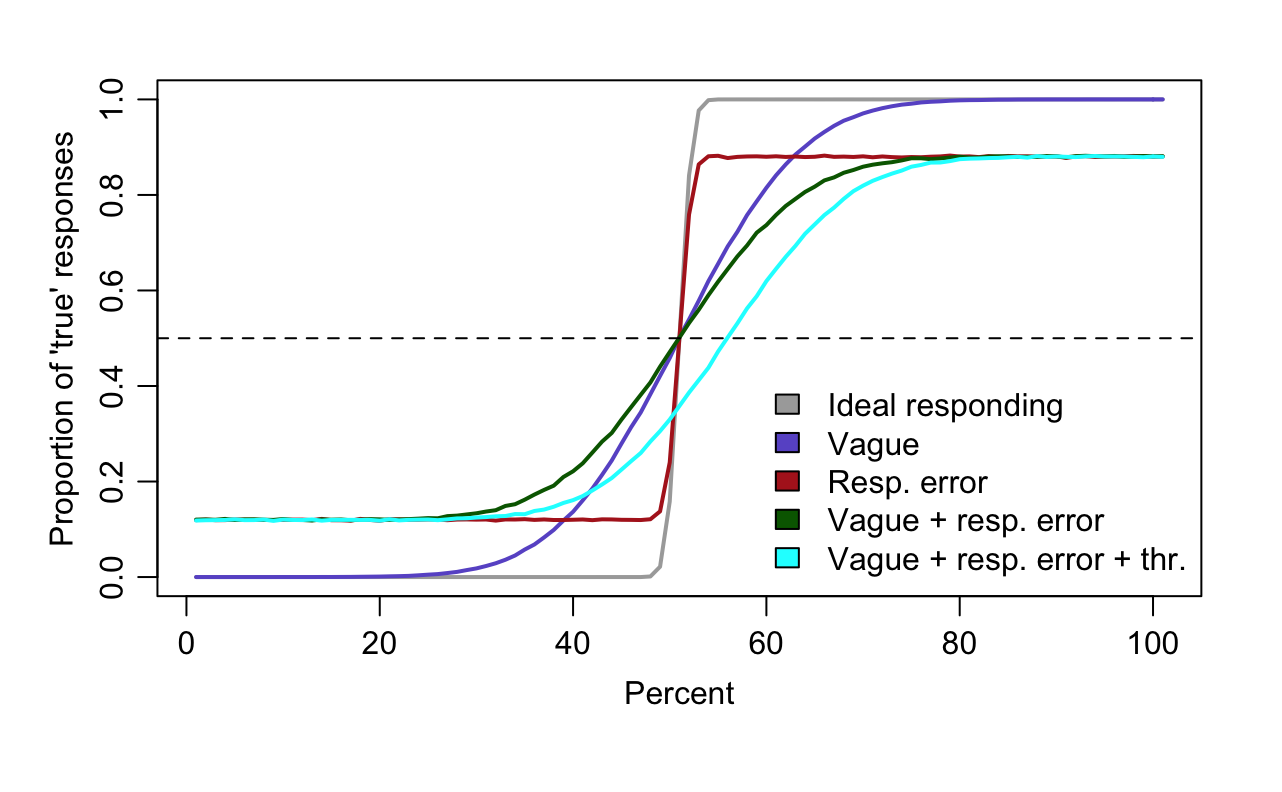
\includegraphics[width=1\textwidth]{Figure2.1.png}
    \caption{Predicted logistic curves under different threshold (thr.), response error (resp. error), and vagueness (vague) parameters. The dashed line indicates the 0.5 proportion of true responses. The percentage for which the logistic curve crosses the dashed line is the threshold.}
    \label{fig:fig2.1}
\end{figure}

\section{Method}
\subsection{Data Availability}
The data and analysis code is available at https://github.com/jstbcs/pling-quant.

\subsection{Participants}
We recruited 90 participants via the online recruitment platform Amazon Mechanical Turk. %https://www.mturk.com/
We excluded 19 participants based on three exclusion criteria. Firstly, we excluded 11 participants who had 50\% or more reaction times faster than 300 ms. Secondly, we excluded 7 participants who failed to obey the monotonicity of quantifiers. We defined the monotonicity criterion in the following way: for positive quantifiers (\textit{many}, \textit{most}, and \textit{more than half}) we expected the probability of providing the true response to increase with increasing proportion. The opposite effect should hold for negative quantifiers. To apply monotonicity criterion, we fitted the generalized linear model to participants' response data with the proportion as a predictor and with by-subject random intercept and slope for proportion (\textit{glmer} R function, \citeNP{Kuznetsova2017LmerTestModels}). We excluded participants, who had a negative slope for positive quantifiers or a positive slope for negative quantifiers. Finally, we excluded 1 participant, who took part in a similar experiment. These exclusions meant that we included 71 participants (47 male, age \textit{M} = 35, range: 22--59) in the final sample. Subjects gave informed consent prior to participation in the experiment. The study was approved by the Ethics Committee of the University of Amsterdam's Faculty of Humanities.

\subsection{Experimental Design and Procedure}
In our experiment, participants had to indicate whether the sentence with the quantifier: \textit{most}, \textit{many}, \textit{few}, \textit{fewer than half}, or \textit{more than half} was true or false based on the sentence containing a proportion ranging from 1\% to 99\% (excluding 50\%). We did not include the proportion 100\%, because \citeA{Ariel2003DoesHalf} showed that \textit{most} has an upper bound on meaning and using it with 100\% proportion is not accepted, although it is highly accepted with 99\%. The upper bound of \textit{most} could cause a divergence in the logistic function which we used in our model. We did not include 50\%, because this proportion could be confusing for \textit{more than half} and \textit{fewer than half}.

While \textit{most}, \textit{more than half} and \textit{fewer than half} have a proportional interpretation \cite{Hackl2009}, as explained above, \textit{many} and \textit{few} are ambiguous between cardinal and proportional reading \cite{Partee1988ManyQuantifiers}. For example, \textit{many} could mean more than a certain number (cardinal reading) or more than a certain proportion (proportional reading, see Example \ref{ex:2.1}). We used explicit partitive `of the' and present proportions as a percentage for all quantifiers to ensure the proportional reading and avoid confounds for ambiguous quantifiers. Moreover, by using the percentage format we enforced the precise comparison between proportion and the threshold. In this way, we minimized the differences between quantifiers in verification strategies. For example, in some experimental paradigms \textit{most} is verified using approximate strategy \cite{Pietroski2009}, while in others mixtures of strategies is used \cite{Talmina2017}.

The experiment started with a short training block to familiarize participants with the procedure. Next participants completed the 250 trials (50 per quantifier) in randomized order. At the end of the experiment, participants provided basic demographic information.
Each trial of the experiment consisted of two sentences displayed on separate screens. The first sentence containing the quantifier was of the form ``[\textit{Most/Many/Few/More than half/Fewer than half}] of the gleerbs are fizzda." To read this sentence participants had to press the arrow down key and keep it pressed. When they advanced to the next screen, they read a sentence containing proportion e.g., ``20\% of the gleerbs are fizzda." Participants had to provide a response by pressing the right or left arrow keys corresponding to true or false judgment (counterbalanced between participants).

In our experiment, we used pseudowords generated from 50 English six-letters nouns and adjectives using \textit{Wuggy} software \cite{Keuleers2010Wuggy:Generator}. We used pseudowords to avoid pragmatic effects associated with quantifiers. The original words were controlled for frequency (\textit{Zipf} value 4.06, \citeNP{vanHeuven2014SUBTLEX-UK:English.}). A native English speaker assessed the pseudowords in terms of how well they imitated English words.

%\hfill \break
%\hfill \break

\subsection{Data pre-processing}
We excluded trials with response times shorter than 300ms and longer than 2500ms (similar cut-offs to \citeNP{Ratcliff2018ModelingModel}). Altogether, we excluded 6\% of trials. To be able to fit the same logit model to all quantifiers we flipped the true and false responses for \textit{few} and \textit{fewer than half}.

\subsection{Computational Model}
The logistic regression model is suitable for modeling the threshold variability \cite{Verheyen2018TypicalityDimensionalAdjectives, Ramotowska2020MostDifferences}. The model assumes that the probability that participants verify a statement as true or false depends on the proportion that was presented on a particular trial and the values of the logistic function parameters asymptote, midpoint and scale:

\begin{equation}
   response \sim \frac{asymptote}{1 + exp(midpoint - proportion)/scale}
\end{equation}

\begin{comment}
\[ \scalebox{2}{$\displaystyle 2 + 2 = 4$} \]
\begin{equation}
    $response \sim \frac{asymptote}{1 + exp(midpoint - proportion)/scale}$
\end{equation}
\end{comment}

To accommodate individual differences and differences between quantifiers in the model, we used a three-parameter logistic regression model inspired by Item Response Theory (IRT). IRT determines the relationship between an individual's trait and the probability of providing a correct response for a given item \cite{Hanlbleton1991FundamentalsData, Ligia2012RelevanceTheory}. This relationship is expressed by the Item Response Function, which maps the IRT parameters (difficulty, discrimination, and guessing) onto the logistic function. The three-parameter model has a difficulty parameter, which determines the level of an individual trait necessary to provide a correct response (midpoint), a discrimination parameter that determines the steepness of the logistic curve (scale), and a guessing parameter that can adjust the logistic curve asymptotes. 

In our model, the threshold corresponds to the difficulty parameter, vagueness to the discrimination parameter, and response error to the guessing parameter from the IRT model. We used a hierarchical Bayesian model to estimate the parameters for each participant-quantifier combination. To fit the model, we used the \textit{rstan} package in R \cite{StanDevelopmentTeam2017Shinystan:Models} %(Stan Development Team, 2020) 
with 6 chains, 750 warm up iterations per chain and 2500 iterations per chain. 

The model was specified in the following way. Let \textit{i} indicate participants, \textit{i} = 1, ..., \textit{I}, \textit{j} indicate the quantifier, \textit{j} = 1, ..., 5, and \textit{k} indicate the trial for each quantifier, \textit{k} = 1, ..., $K_{ij}$. Then $Y_{ij}$ is the \textit{i}-th participant's response to the \textit{j}-th quantifier in the \textit{k}-th trial, and $Y_{ijk} = 1$ if participant indicated true, and $Y_{ijk} = 0$ if participant indicated false. Then, we may model $Y_{ijk}$ as a Bernoulli, using the logit link function on the probabilities:

\begin{equation}
    Y_{ijk} \sim Bernoulli(\pi_{ijk})
\end{equation}

where the probability space of $\pi$ maps onto the $\mu$.

\begin{equation}
    \pi_{ijk} = \gamma_{ij} + (1-2\gamma_{ij})logit^-1(\mu_{ijk})
\end{equation}

The additional parameter $\gamma_{ij}$ determines the probability of making a response error on either side of the threshold, namely erroneously saying true, or erroneously saying false. Each participant-quantifier combination has its own response error parameter estimate. The parameter $\mu_{ijk}$ has a linear model explication:

\begin{equation}
    \mu_{ijk} = \frac{c_{ijk} - \beta_{ij}}{\alpha_{ij}}
\end{equation}

where $c_{ijk}$ indicates the percentage centered at 50\%,  parameters $\beta_{ij}$ indicate the threshold, and parameters $\alpha_{ij}$ correspond to the vagueness of the quantifier.

We defined prior probabilities on response error ($\gamma$), threshold ($\beta$), and vagueness ($\alpha$) parameters:

\begin{subequations}
\begin{equation}
    \gamma_{ij} \sim Beta(2, 20)
\end{equation}
\begin{equation}
     \beta_{ij} \sim Normal(\delta_j, \sigma^2_j)
\end{equation}
\begin{equation}
    \alpha_{ij} \sim log-Normal(\nu_j, \sigma^2_{\alpha_j})
\end{equation}
\begin{equation}
    \nu_j \sim Normal(0, 5^2)
\end{equation}
\begin{equation}
    \sigma^2_{\alpha_j} \sim Invers-Gamma(2, 0.2)
\end{equation}
\begin{equation}
    \sigma^2_j \sim Invers-Gamma(2, 0.2)
\end{equation}
\begin{equation}
    \delta_j \sim Normal(0, 5^2)
\end{equation}
\end{subequations}

The hierarchical nature of the distributions for $\alpha_{ij}$ and $\beta_{ij}$ indicate that we estimated the effect of threshold and vagueness for each participant under the assumption that they had a common mean and variance. The vagueness and threshold priors were fairly uninformative to avoid the inclusion of incidental constraints. Vagueness ($\alpha_{ij}$) came from a log-normal distribution to ensure only the positive estimates. Its mean ($\nu_j$) had a normal distribution, and its variance ($\sigma^2_{\alpha_j}$) was drawn from Inverse-Gamma distribution, as this distribution is typically used to model variance. For the thresholds ($\beta_{ij}$) we used a normal distribution with a common, normally-distributed mean ($\delta_j$) and the same variance distribution ($\sigma^2_j$) as for $\alpha_{ij}$. The response error ($\gamma_{ij}$) came from a more informed distribution with most of its mass below an error rate of 20\% for each true and false response\footnote{To reduce the complexity of the model, we did not use hierarchical modeling for response errors.}. 

\subsection{Cluster analysis}
We ran an exploratory cluster analysis for the threshold parameter\footnote{See cluster analysis for vagueness and response errors in Appendix.} estimating the clusters using the k-means clustering method (\textit{kmeans} function in R, \citeNP{Hartigan1979AlgorithmAlgorithm}). We determined the optimum number of clusters by using the elbow plots and Silhouette width. We chose the k-mean clustering because it could be apply to relatively small data set and does not impose too much structure into the data \cite{Weigand2021}.

\subsection{Linear Discriminant Analysis}
To assess the contribution of the model estimates to the clustering, we performed a linear discriminant analysis (LDA). We used the stepwise procedure Wilks' lambda assessment (\textit{greedy.wilks} function in R package \textit{klaR}, \citeNP{Roever2015PackageVisualization}) to determine which variable contributed significantly to cluster formation. Next, we ran the LDA (\textit{lda} function in R package \textit{MASS}) to test how accurately the selected variables could predict the clusters. To validate the LDA, we ran a leave-one-out cross validation.

\section{Results}
\subsection{Estimated parameters}
The estimated model parameters are shown in Table \ref{tab:tab2.1}. Figure \ref{fig:fig2.2} shows the estimated  item response curves for each participant-quantifier combination; the overall response curves for the quantifiers are represented by the bold, colored lines. We found greater individual variation in thresholds for \textit{most}, \textit{many} and \textit{few}, compared to \textit{more than half} and \textit{fewer than half}. At the group level, quantifier thresholds were represented in the following order (Friedman test $\chi^2(4) = 134$, \textit{p} $< 0.001$, moderate effect size \textit{W} = 0.47): \textit{few} had the lowest threshold, followed by \textit{many}, then were \textit{fewer than half} and \textit{more than half}, and \textit{most} had the highest threshold (pairwise comparison, Wilcoxon Signed Rank Test with Bonferroni correction).

\begin{table}[H]
    \centering
    \caption{Mean (\textit{SD}) parameters of individual participants for each quantifier, and additionally for threshold parameter the percent corresponding to mean thresholds.}
    \label{tab:tab2.1}
    \begin{tabular}{lcccc}\hline
         & Threshold & Vagueness & Response error  \\ \hline
         \textit{Few} & -.103 (.073), 39.7\%  & .016 (.001) & .062 (.042)\\
         \textit{Fewer than half} & -.006 (.027),
49.4\% & .002 (.00004) & .074 (.047)\\
         \textit{Many} & -.061 (.094)
43.9\% & .019 (.003) & .048 (.024)\\
         \textit{More than half} & .001 (.012)
50.1\% & .001 (.00003) & .042 (.019)\\
         \textit{Most} & .029 (.056)
52.9\% & .009 (.001) & .047 (.024)\\ \hline
    \end{tabular}
\end{table}

The quantifiers \textit{fewer than half} and \textit{more than half} were the least vague as indicated by the steep response curves in Figure \ref{fig:fig2.2}. Moreover, \textit{few} was more vague than \textit{fewer than half} (\textit{V} = 2556; \textit{p} $< 0.001$), \textit{many} was more vague than \textit{more than half} (\textit{V} = 2556; \textit{p} $< 0.001$), \textit{many} was more vague than \textit{most} (\textit{V} = 2556; \textit{p} $< 0.001$), and \textit{most} was more vague than \textit{more than half} (\textit{V} = 2556; \textit{p} $< 0.001$), \textit{p} - values based on Wilcoxon Signed Rank Test. We also found that \textit{fewer than half} had a greater response error than \textit{more than half} (\textit{V} = 2323; \textit{p} $< 0.001$), and \textit{few} had greater response error than \textit{many} (\textit{V} = 1809; \textit{p} = 0.002), \textit{p} - values based on Wilcoxon Signed Rank Test. As predicted, the vague quantifiers had a higher value of vagueness parameter and negative quantifiers had higher value of response error parameter.

\begin{figure} [H]
    \centering
    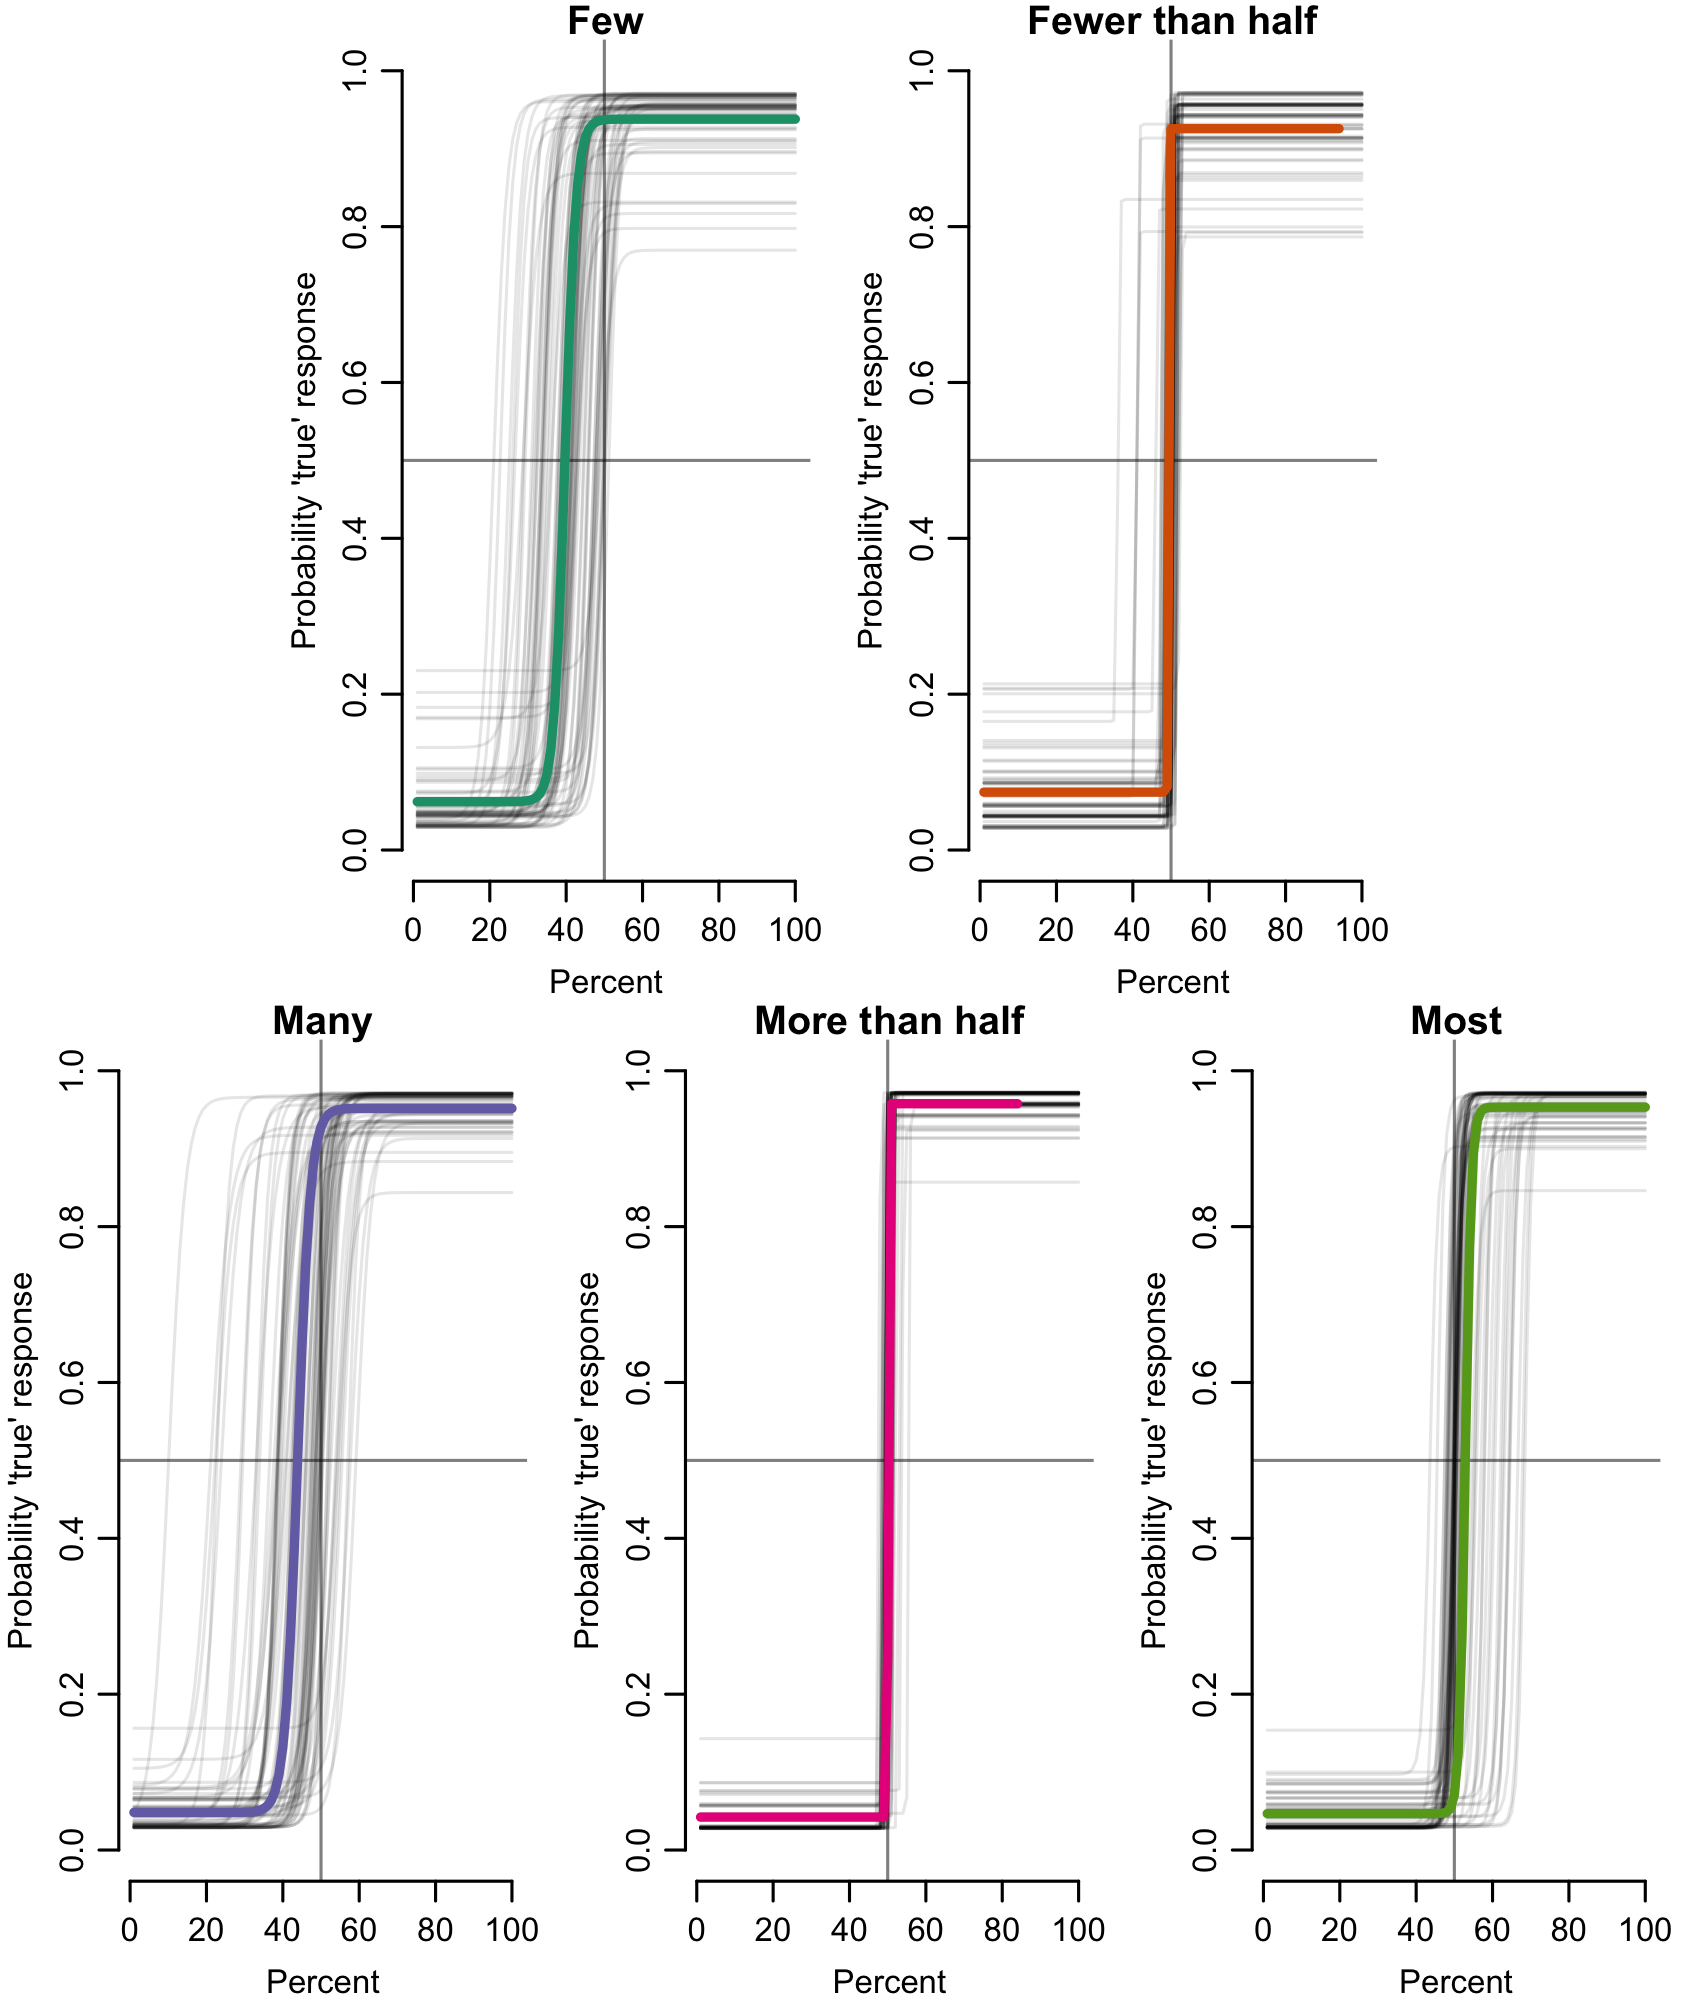
\includegraphics[width=\textwidth, height=16cm]{Figure2.2.png}
    \caption{The logit curves estimated for each quantifier. The color lines indicate the mean curves.}
    \label{fig:fig2.2}
\end{figure}

\subsection{Individual differences in thresholds}
%In the next step, we studied the associations between model parameters across quantifiers to reveal potentially systematic patterns (see Figure \ref{fig:fig2.3}). 
In the next step, we explored the associations between threshold parameter across quantifiers to reveal potentially systematic patterns (see Figure \ref{fig:fig2.3}).
%Figure \ref{fig:fig2.3a} shows the correlations between thresholds. 
The Pearson correlations between thresholds were negligible or weak. The lack of significant correlations between thresholds of \textit{fewer than half} and \textit{more than half} and other quantifiers is not surprising given a little between-participants variability in truth conditions of \textit{fewer than half} and \textit{more than half}. The lack of correlations between thresholds of vague quantifiers requires a comment.
A significant positive correlation between thresholds would indicate individual differences in preference toward placing the thresholds high or low on a mental scale for all quantifiers (e.g., the higher threshold for \textit{many}, the higher threshold for \textit{few}). A significant negative correlation would indicate individual differences in distance between thresholds (e.g., a high threshold for \textit{many} and a low threshold for \textit{few} indicate greater distance, while a low threshold for \textit{many} and a high threshold for \textit{few} indicate smaller distance). %Our finding, in turn, suggests that clusters of participants could have different representation and ordering on the mental line. 
Our analysis did not reveal systematic patterns. Therefore, it gives additional reason for the cluster analysis, because the lack of correlation might be caused by different position of thresholds in the subgroups.

\begin{figure} [H]
    \centering
   % 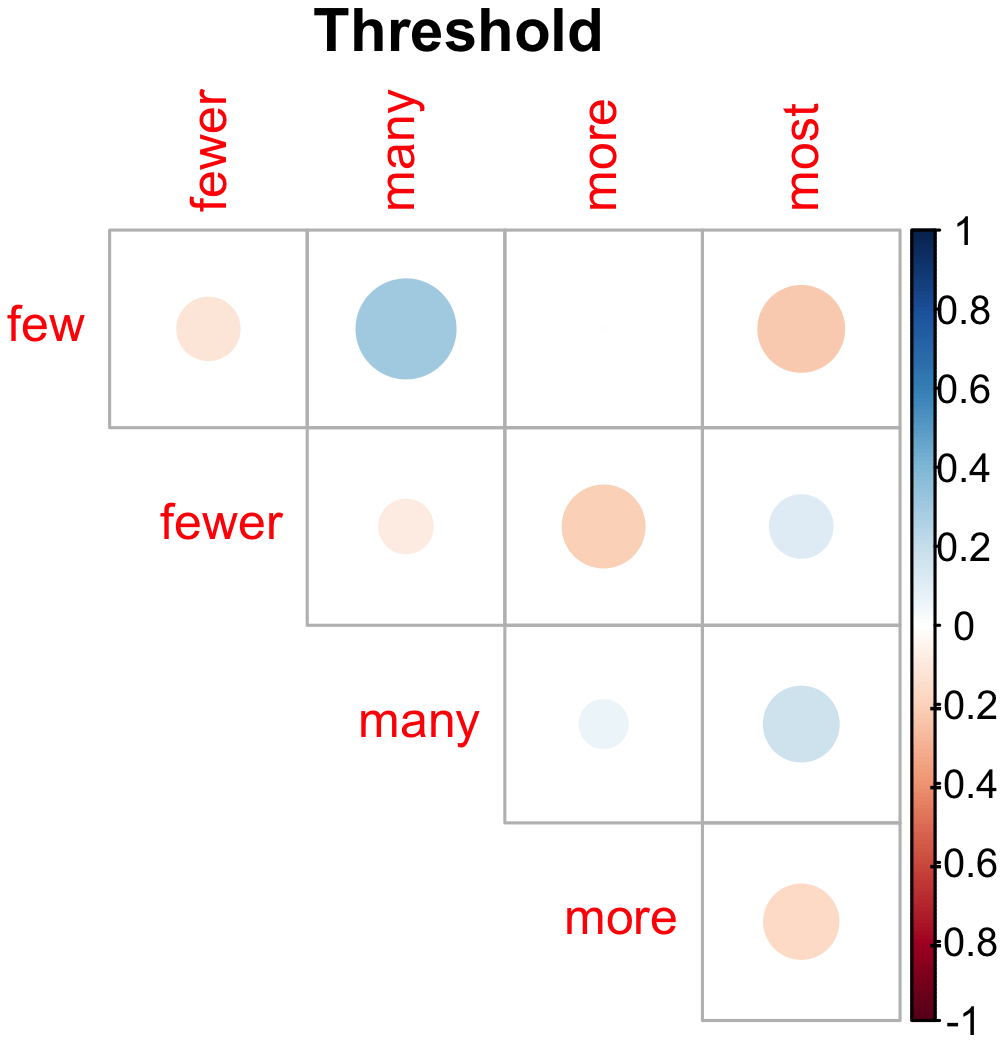
\includegraphics[width=\textwidth]{Figure2.3a.png}
   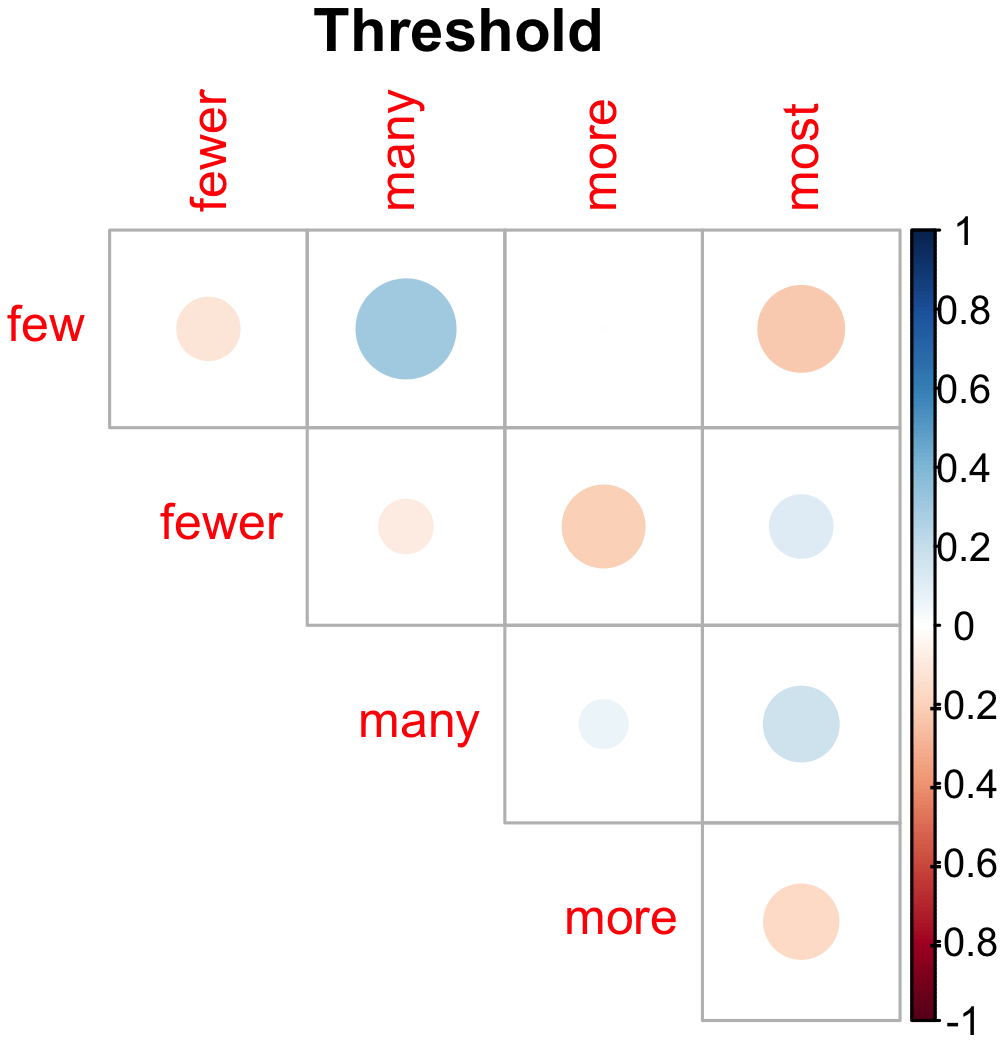
\includegraphics[scale=0.25]{Figure2.3a.png}
    \caption{The Pearson correlations between thresholds (significance level *** 0.001, ** 0.01,*  0.05). The \textit{p} -  values were adjusted using the Bonferroni correction.}
    \label{fig:fig2.3}
\end{figure}

\iffalse
\begin{figure} [H]
   \begin{minipage}[t]{\textwidth}
   \begin{minipage}[t]{0.49\textwidth}
    \begin{subfigure}[t]{\linewidth}
     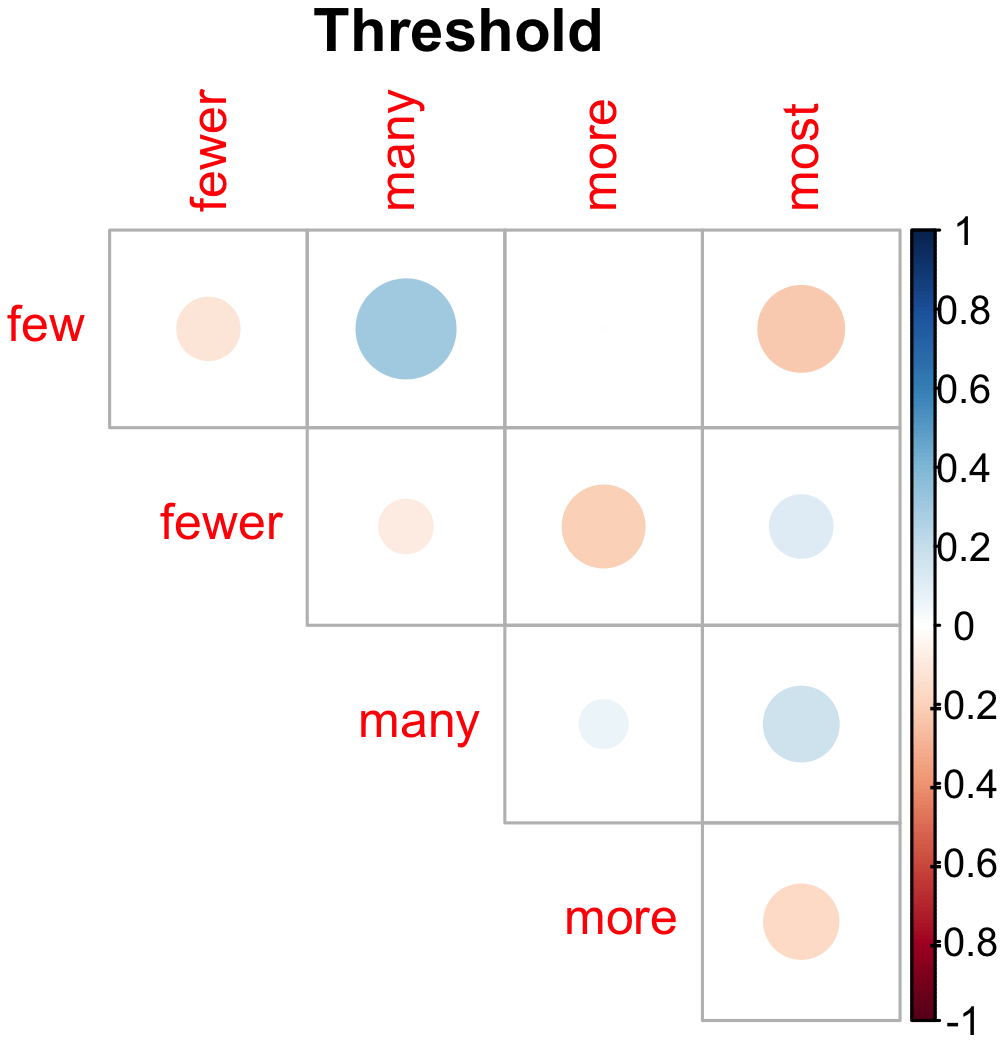
\includegraphics[width=\linewidth]{Figure2.3a.png}
     \caption{\label{fig:fig2.3a}}
    \end{subfigure}

    \begin{subfigure}[t]{\linewidth}
     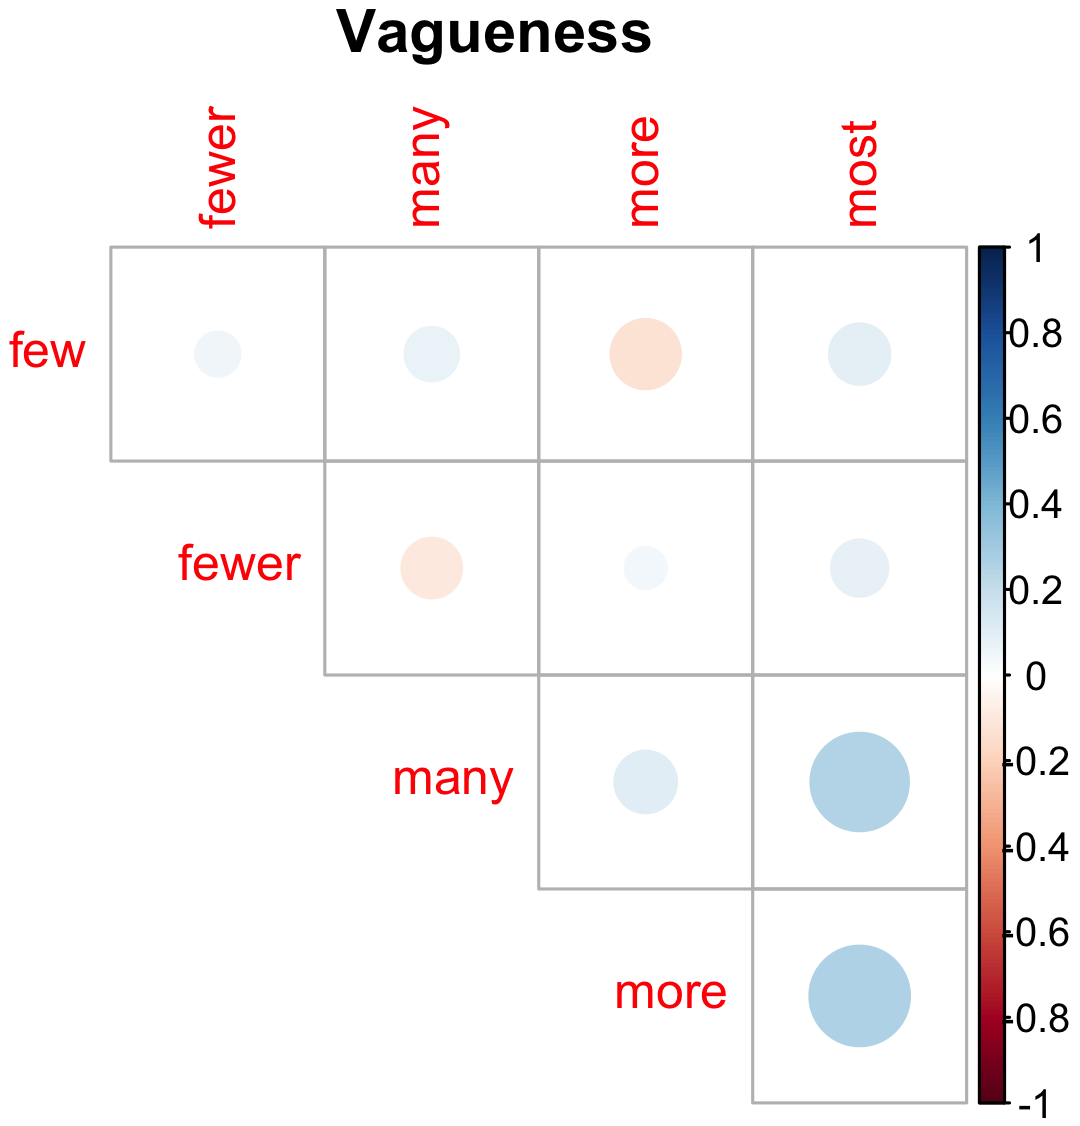
\includegraphics[width=\linewidth]{Figure2.3b.png}
     \caption{\label{fig:fig2.3b}}
    \end{subfigure}
    \end{minipage}
    \hfill
    \begin{minipage}[t]{0.49\textwidth}
    \begin{subfigure}[t]{\linewidth}
     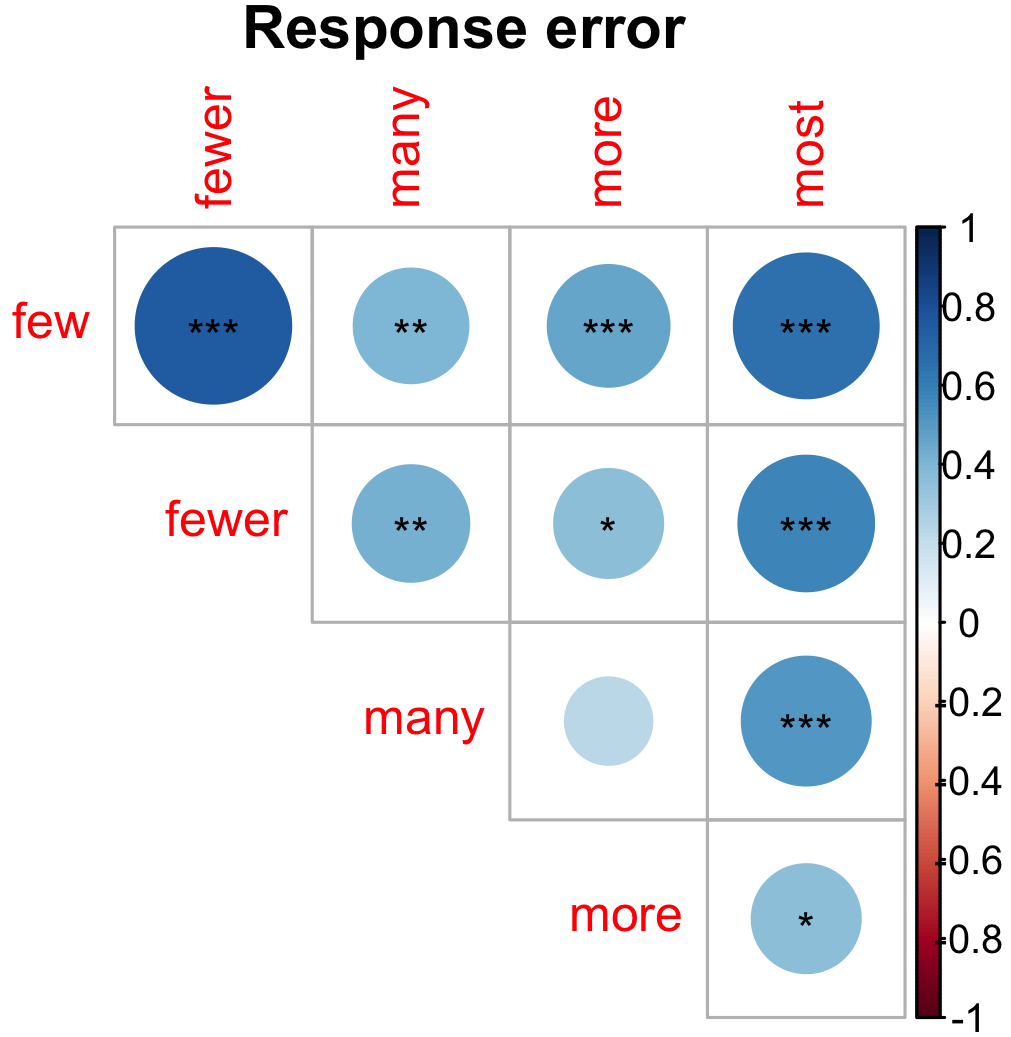
\includegraphics[width=\linewidth]{Figure2.3c.png}
     \caption{\label{fig:fig2.3c}}
    \end{subfigure}
    \end{minipage}
   \end{minipage}
    \caption{\ref{fig:fig2.3a} Correlations between thresholds; \ref{fig:fig2.3b} correlations between vagueness; \ref{fig:fig2.3c} correlations between response error (significance level *** 0.001, ** 0.01,*  0.05). The \textit{p} values were adjusted using the Bonferroni correction.}
    \label{fig:fig2.3}
\end{figure}
\fi

\subsubsection{Cluster analysis results}
%\subsubsection{Threshold}
Following the correlation analysis we performed the k-mean clustering on the threshold parameter from all quantifiers. This analysis addressed our first research question concerning the subgroups of participants. We hypothesized that participants will cluster into groups with aligned meanings.

The methods to determine the optimum number of clusters for threshold gave ambiguous results. The elbow plot indicated 3 or 4 clusters, while the Silhouette method preferred 5 clusters. We chose the simplest solution, comprising 3 clusters, because the additional clusters consisted of only 4 participants, making interpretation difficult. The three clusters were indistinguishable for the quantifiers \textit{fewer than half} and \textit{more than half}, but differed substantially in thresholds for the quantifiers \textit{few}, \textit{many}, and \textit{most}. %Figure \ref{fig:fig2.5} shows the individual estimates for threshold, vagueness, and response error parameters for the quantifiers \textit{few}, \textit{many}, and \textit{most}, with color indicating cluster membership.

The first cluster (\textit{N} = 13) consisted of participants with a higher mean threshold for \textit{most} and a lower threshold for \textit{few}, the second cluster (\textit{N} = 34) included participants who had thresholds for all quantifiers close to 50\%, and the last cluster (\textit{N} = 24) consisted of participants who had similar a mean threshold for \textit{few} and \textit{many} (see Table \ref{tab:tab2.2}). %In addition, we found that participants in Cluster 3 had a higher tendency to make errors, with this tendency especially visible for \textit{few} (see Figure \ref{fig:fig2.5}).

\begin{table}[H]
    \centering
    \caption{Mean (\textit{SD}) threshold parameter in each cluster and percentage corresponding to mean thresholds, 3-cluster solution.}
    \label{tab:tab2.2}
    \begin{tabular}{lcccc}\hline
         Quantifier & Cluster 1  & Cluster 2  & Cluster 3 \\
          & (\textit{N} = 13) & (\textit{N} = 34) & (\textit{N} = 24) \\ \hline
         \textit{Few} & -.15 (.05) & -.05 (.04) & -.15 (.07)\\
          &  35\% &  45\% &  35\%\\
         \textit{Fewer than half} & .001 (.01) & -.012 (.03) & -.002 (.02)\\
         & 50.1\% & 48.8\% & 49.8\%\\
         \textit{Many} & .014 (.06) & -.022 (.04) & -.16 (.09)\\
         & 51.4\% & 47.8\% & 34\%\\
         \textit{More than half} & -.00006 (.006) & .002 (.01) & .0007 (.01) \\
         & 49.99\% & 50.2\% & 50.07\% \\
         \textit{Most} & .10 (.05) & .009 (.03) & .02 (.05)\\ 
         & 60\% & 50.9\% & 52\%\\\hline
    \end{tabular}
\end{table}

\iffalse
\begin{figure} [H]
 \centering
     \begin{subfigure}[b]{0.99\textwidth}
     \centering
     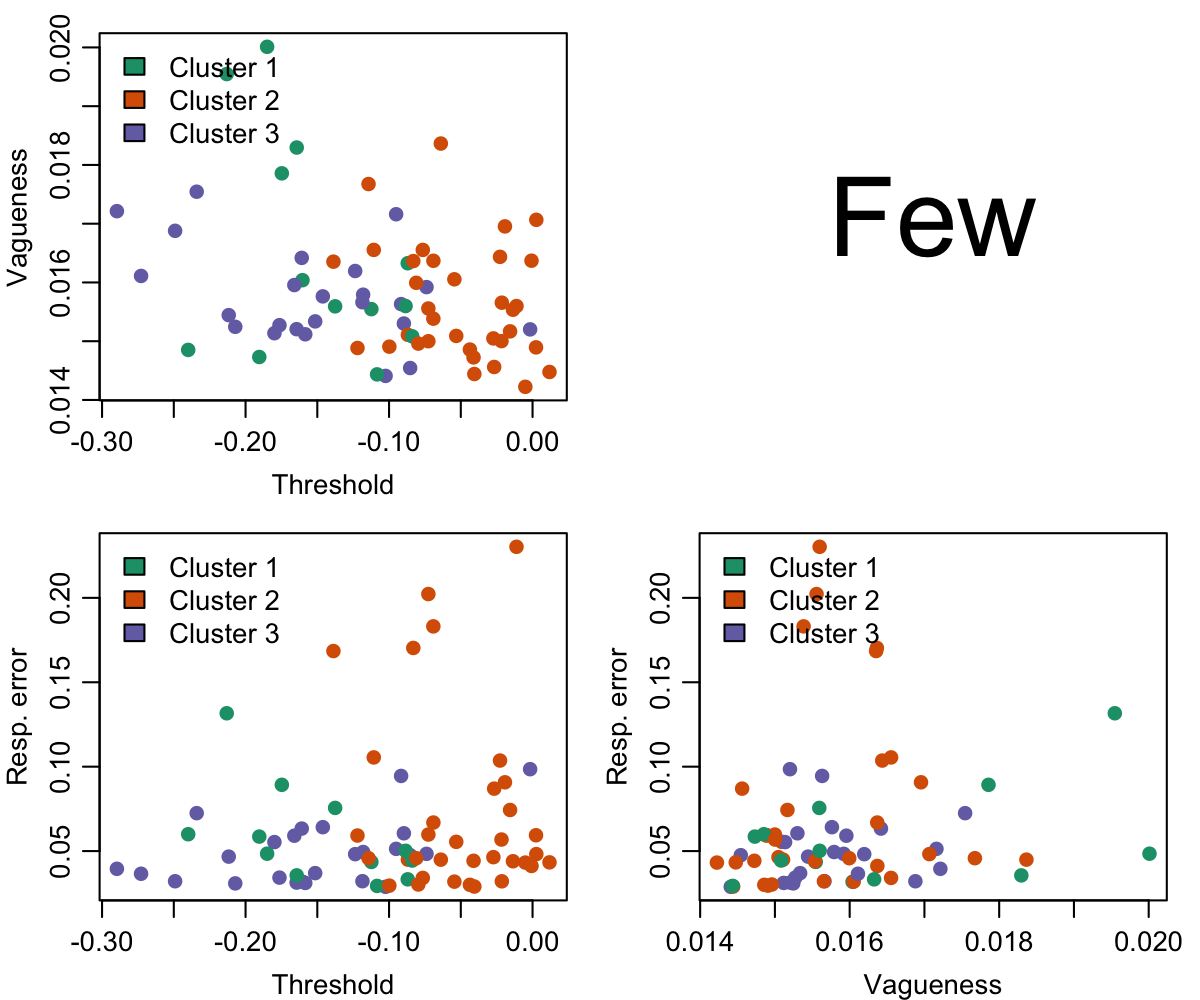
\includegraphics[width=\textwidth]{Figure2.5a.png}
     \caption{\label{fig:fig2.5a}}
    \vspace{4ex}
    \end{subfigure}
    
    \begin{subfigure}[b]{0.99\textwidth}
    \centering
     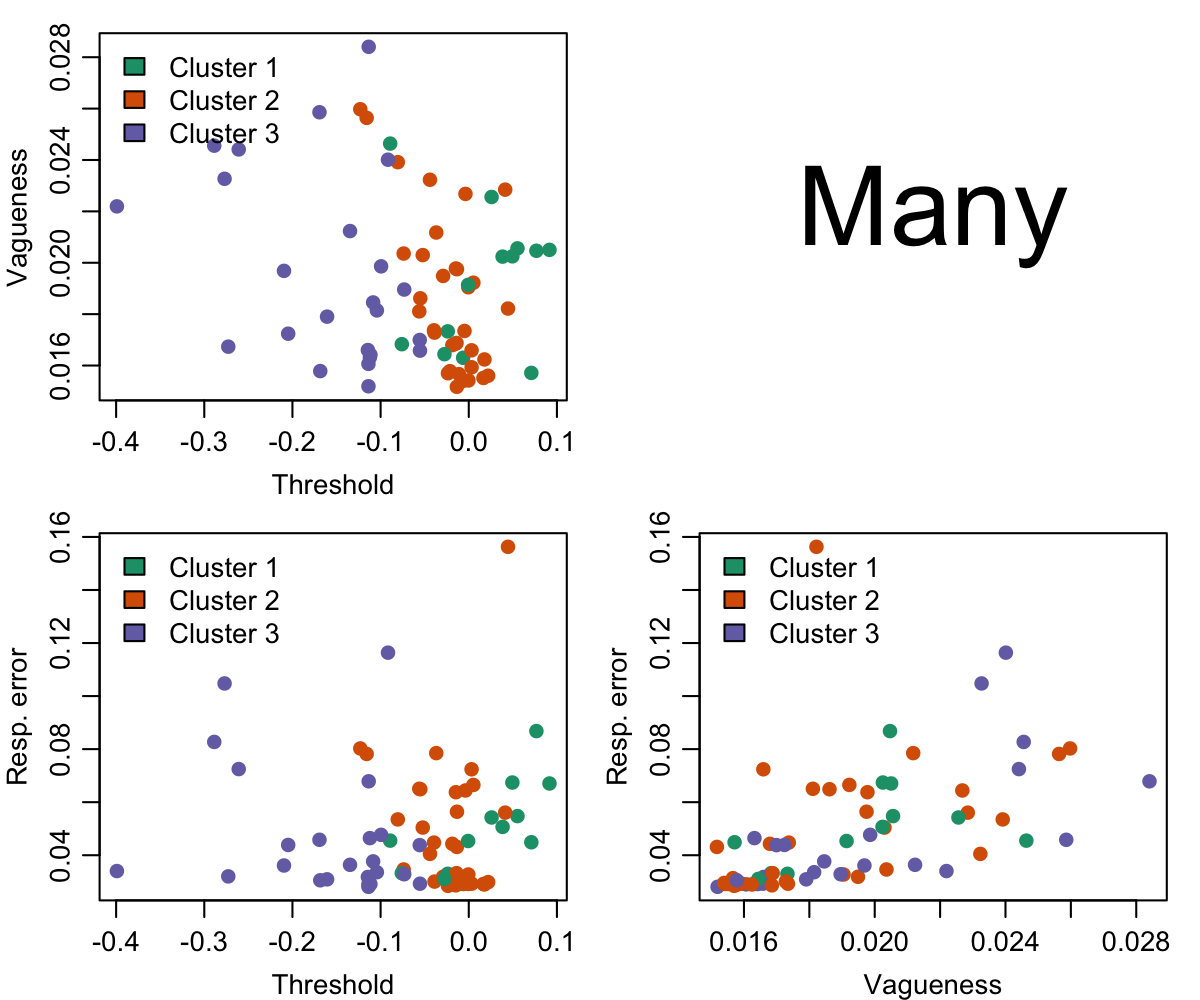
\includegraphics[width=\linewidth]{Figure2.5b.png}
     \caption{\label{fig:fig2.5b}}
    \vspace{4ex}
    \end{subfigure}
\end{figure}

\begin{figure} [H]\ContinuedFloat
\centering
    \begin{subfigure}[b]{0.99\textwidth}
    \centering
     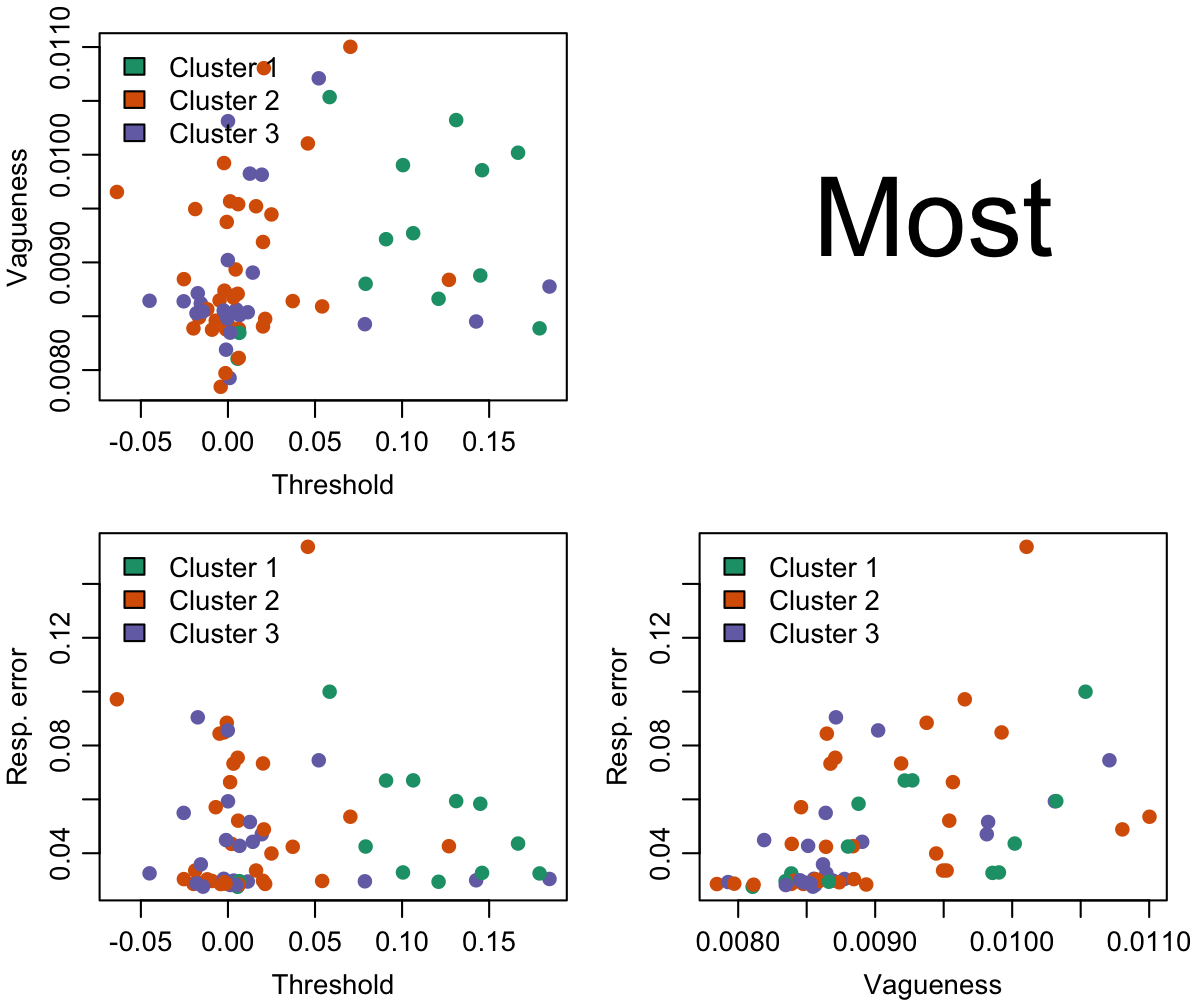
\includegraphics[width=\linewidth]{Figure2.5c.png}
     \caption{\label{fig:fig2.5c}}
    \end{subfigure}
  %  \end{minipage}
    \caption{Relationship between threshold, vagueness, and response error for \textit{few} (\ref{fig:fig2.5a}), \textit{many} (\ref{fig:fig2.5b}), and \textit{most} (\ref{fig:fig2.5c}), indicating three clusters based on threshold. Cluster 1 (\textit{N} = 13) is indicated in green, Cluster 2 (\textit{N} = 34) in orange, Cluster 3 (\textit{N} = 24) in purple.}
    \label{fig:fig2.5}
\end{figure}
\fi

\subsubsection{Linear Discriminant Analysis results}
%\subsubsection{Threshold}
For thresholds, as expected, we found that only vague quantifiers contributed to the clustering: \textit{many} ($\lambda$ = 0.42, \textit{p} $<$ 0.001), \textit{few} ($\lambda$ = 0.24, \textit{p} $<$ 0.001), and  \textit{most} ($\lambda$ = 0.16, \textit{p} $<$ 0.001). Figure \ref{fig:fig2.9} shows the combined effect of the three quantifiers on the clustering. The LDA accuracy in classification into Clusters 1 to 3 based on thresholds for \textit{many}, \textit{few} and \textit{most} was 97\%, and the leave-one-out cross validation accuracy was 94\%.

\begin{figure} [H]
    \centering
    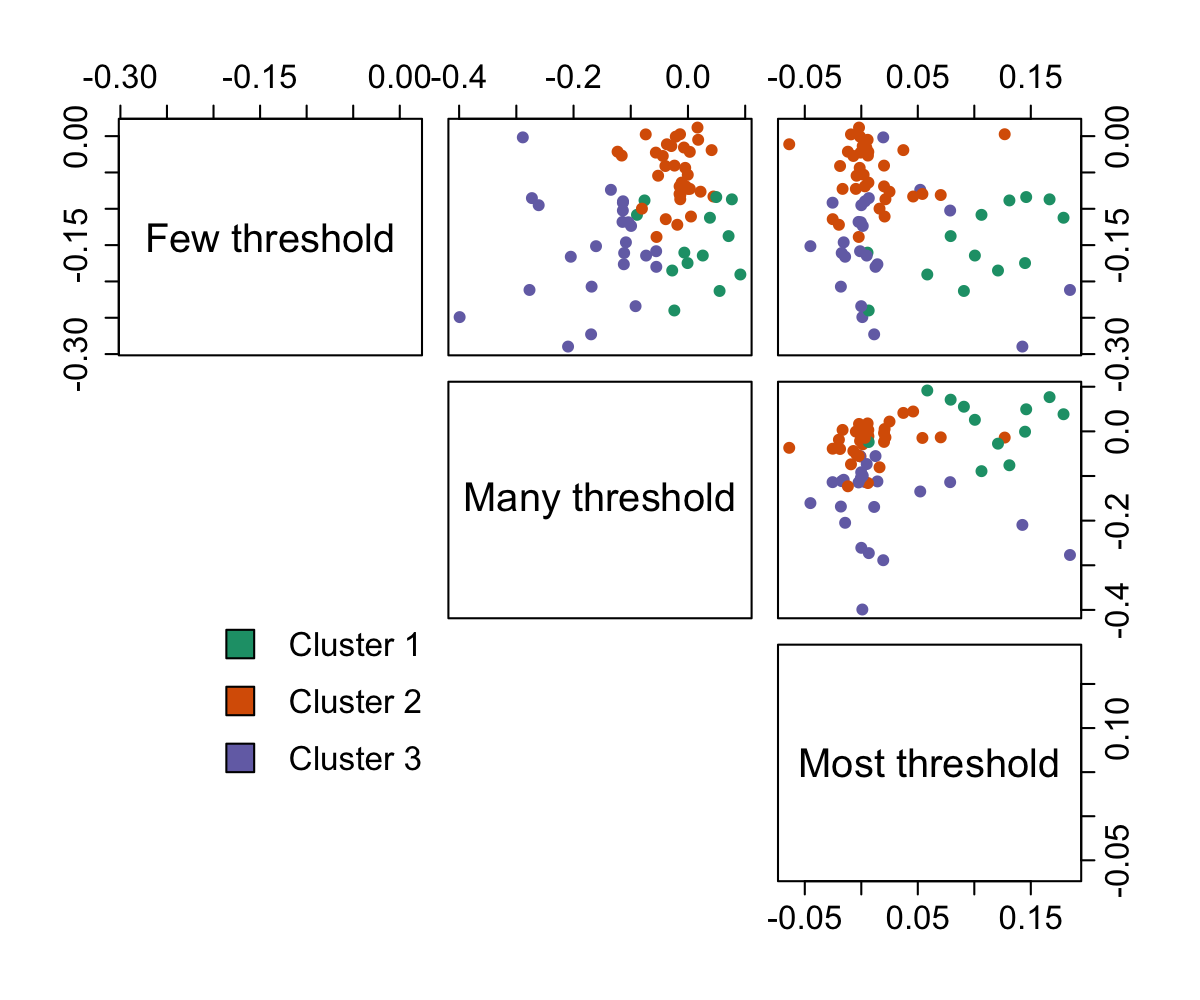
\includegraphics[width=\textwidth]{Figure2.9.png}
    \caption{Three clusters for threshold based on \textit{few}, \textit{many}, and \textit{most} parameters. The parameters' values of thresholds for three quantifiers (\textit{few}, \textit{many}, and \textit{most}) that contributed to clustering are plotted against each other. Colors are used to indicate the cluster membership: Cluster 1 (\textit{N} = 13) is indicated in green, Cluster 2 (\textit{N} = 34) in orange, and Cluster 3 (\textit{N} = 24) in purple.}
    \label{fig:fig2.9}
\end{figure}

\subsection{Mental line of quantifiers}
Our second research question concerned the order of quantifiers on a mental line in the subgroups of participants. %Because we did not find a systematic relationship between thresholds of different quantifiers (see Figure \ref{fig:fig2.3}), we investigated this relationship in the clusters (see Figure \ref{fig:fig2.6}). We tested whether that the lack of correlations between thresholds could be explained by the difference in distance between quantifiers in subgroups. 
We investigated whether all participants would have the same order of vague quantifiers on a mental line. Figure \ref{fig:fig2.6a} shows that all participants had a lower or equal thresholds for \textit{many} than for \textit{most}. However, the distance between thresholds was higher in Cluster 3 than in other clusters. Figure \ref{fig:fig2.6b} shows that the vast majority had a higher threshold for \textit{many} than for \textit{few}. The greatest distance between thresholds was in Cluster 1, while the smallest was in Cluster 3. Figures \ref{fig:fig2.6c} and \ref{fig:fig2.6d} show that all participants in Cluster 3 had a lower threshold for \textit{many} than for \textit{more than half} and \textit{fewer than half}. In sum, the results indicate a rather stable order of quantifiers among three clusters, however, the distance between thresholds varies substantially among clusters.

\begin{figure} [H]
   % \begin{minipage}[b]{0.45\textwidth}
    
    \begin{subfigure}[b]{0.85\textwidth}
     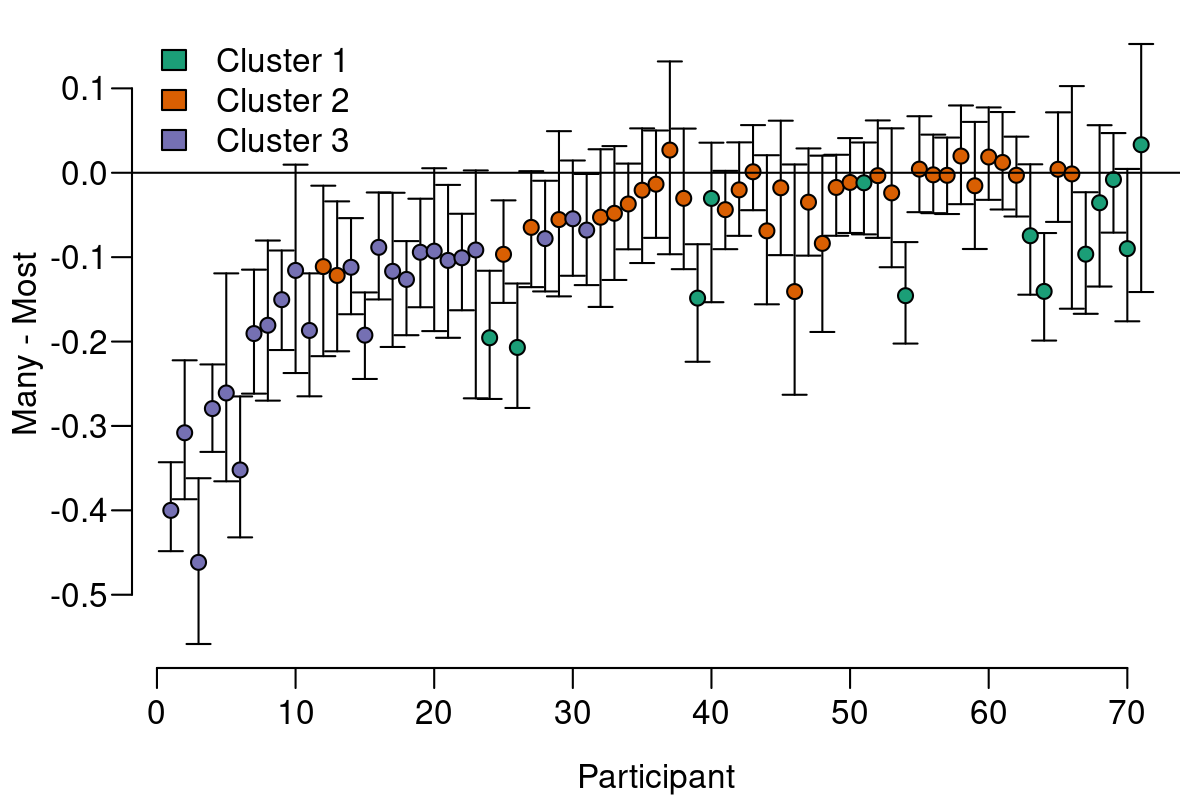
\includegraphics[width=\linewidth]{Figure2.6a.png}
     \caption{\label{fig:fig2.6a}}
    \end{subfigure}
    
    %\vspace{4ex}
    \begin{subfigure}[b]{0.85\textwidth}
     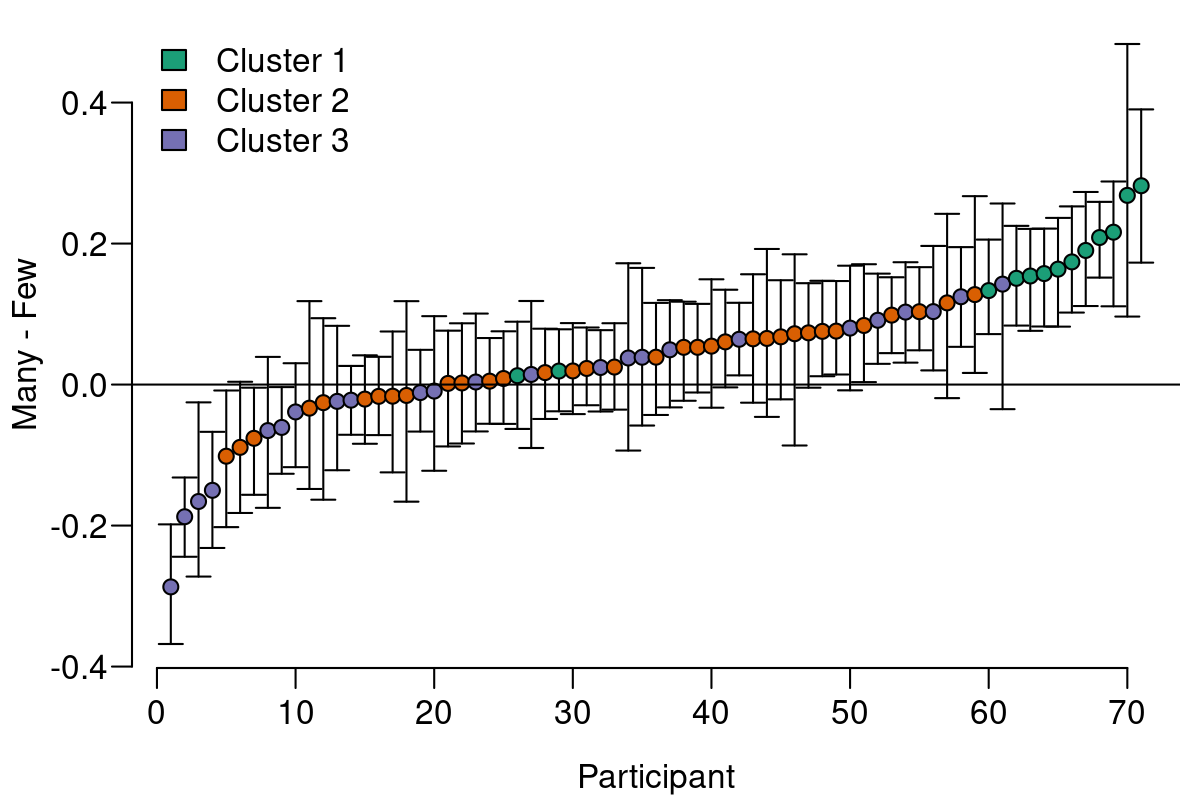
\includegraphics[width=\linewidth]{Figure2.6b.png}
     \caption{\label{fig:fig2.6b}}
    \end{subfigure}
\end{figure}
  %  \end{minipage}
  %  \hfill
 \begin{figure}[H] \ContinuedFloat
   % \begin{minipage}[b]{0.45\textwidth}
    \begin{subfigure}[b]{0.85\textwidth}
     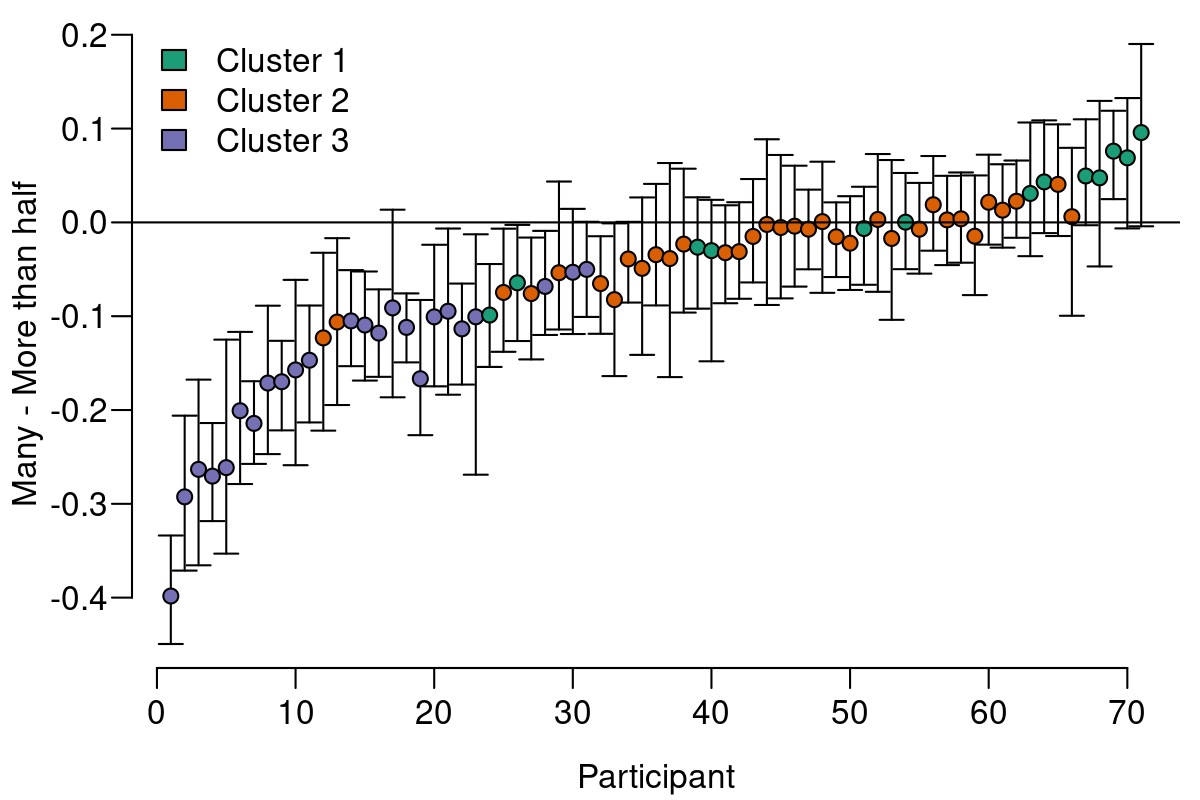
\includegraphics[width=\linewidth]{Figure2.6c.png}
     \caption{\label{fig:fig2.6c}}
    \end{subfigure}
    
 %   \vspace{4ex}
    \begin{subfigure}[b]{0.85\textwidth}
     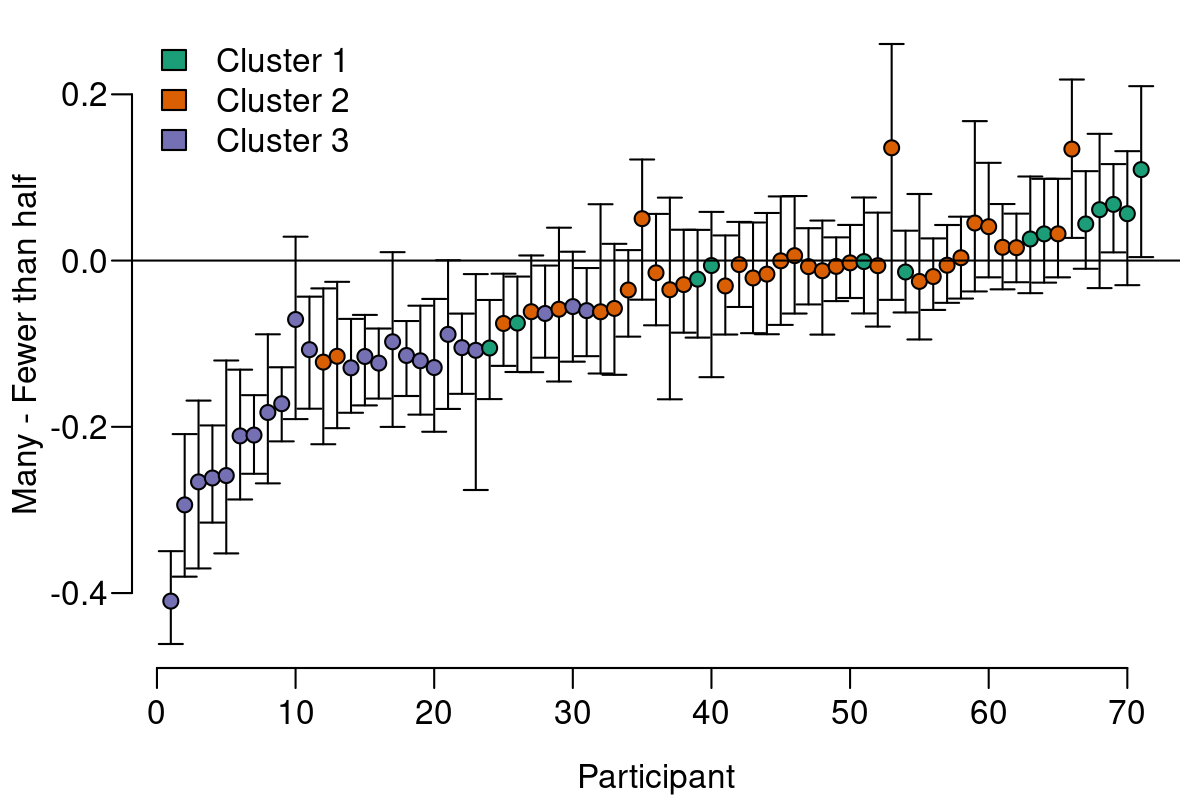
\includegraphics[width=\linewidth]{Figure2.6d.png}
     \caption{\label{fig:fig2.6d}}
    \end{subfigure}
  %  \end{minipage}
    \caption{Differences between individual thresholds ordered from smallest to largest. \textbf{a.} The difference between the threshold for \textit{many} and \textit{most}. \textbf{b.} The difference between the threshold for \textit{many} and \textit{few}. \textbf{c.} The difference between the threshold for \textit{many} and \textit{more than half}. \textbf{d.} The difference between the threshold for \textit{many} and \textit{fewer than half}. Colors are used to indicate cluster membership: Cluster 1 is indicated in green (\textit{N} = 13), Cluster 2 in orange (\textit{N} = 34), and Cluster 3 in purple (\textit{N} = 24). The error bars indicate the 95\% credible intervals.}
    \label{fig:fig2.6}
\end{figure}

\subsection{The interrelationship between vagueness, threshold, and response error}
Finally, we addressed our third research question about the interrelationship between vagueness, threshold, and response error. We correlated the model parameters for each quantifier (Figure \ref{fig:fig2.4}). Although this analysis was exploratory in nature, it gave additional rationale for our modeling choices. Significant high correlations between all parameters of our model would be problematic. It would mean that the parameters of our model do not capture unique source of variability in the data. Thus a more parsimonious model would be desired. Therefore, we wanted to test whether there were any systematic patterns of correlations between parameters across quantifiers. We found a significant negative correlation between threshold and vagueness for \textit{few} (\textit{r} = -0.33) and \textit{many} (\textit{r} = -0.31). We also found correlations between threshold and response error for \textit{fewer than half} (\textit{r} = -0.32), and response error and vagueness for \textit{many} (\textit{r} = 0.53) and \textit{most} (\textit{r} = 0.52). In general, the correlations did not reveal systematic patterns across quantifiers. The lack of systematic correlations between vagueness and response error parameters gives additional support to the choice to model these parameters as two separate mechanisms.

\begin{figure} [H]
    \centering
    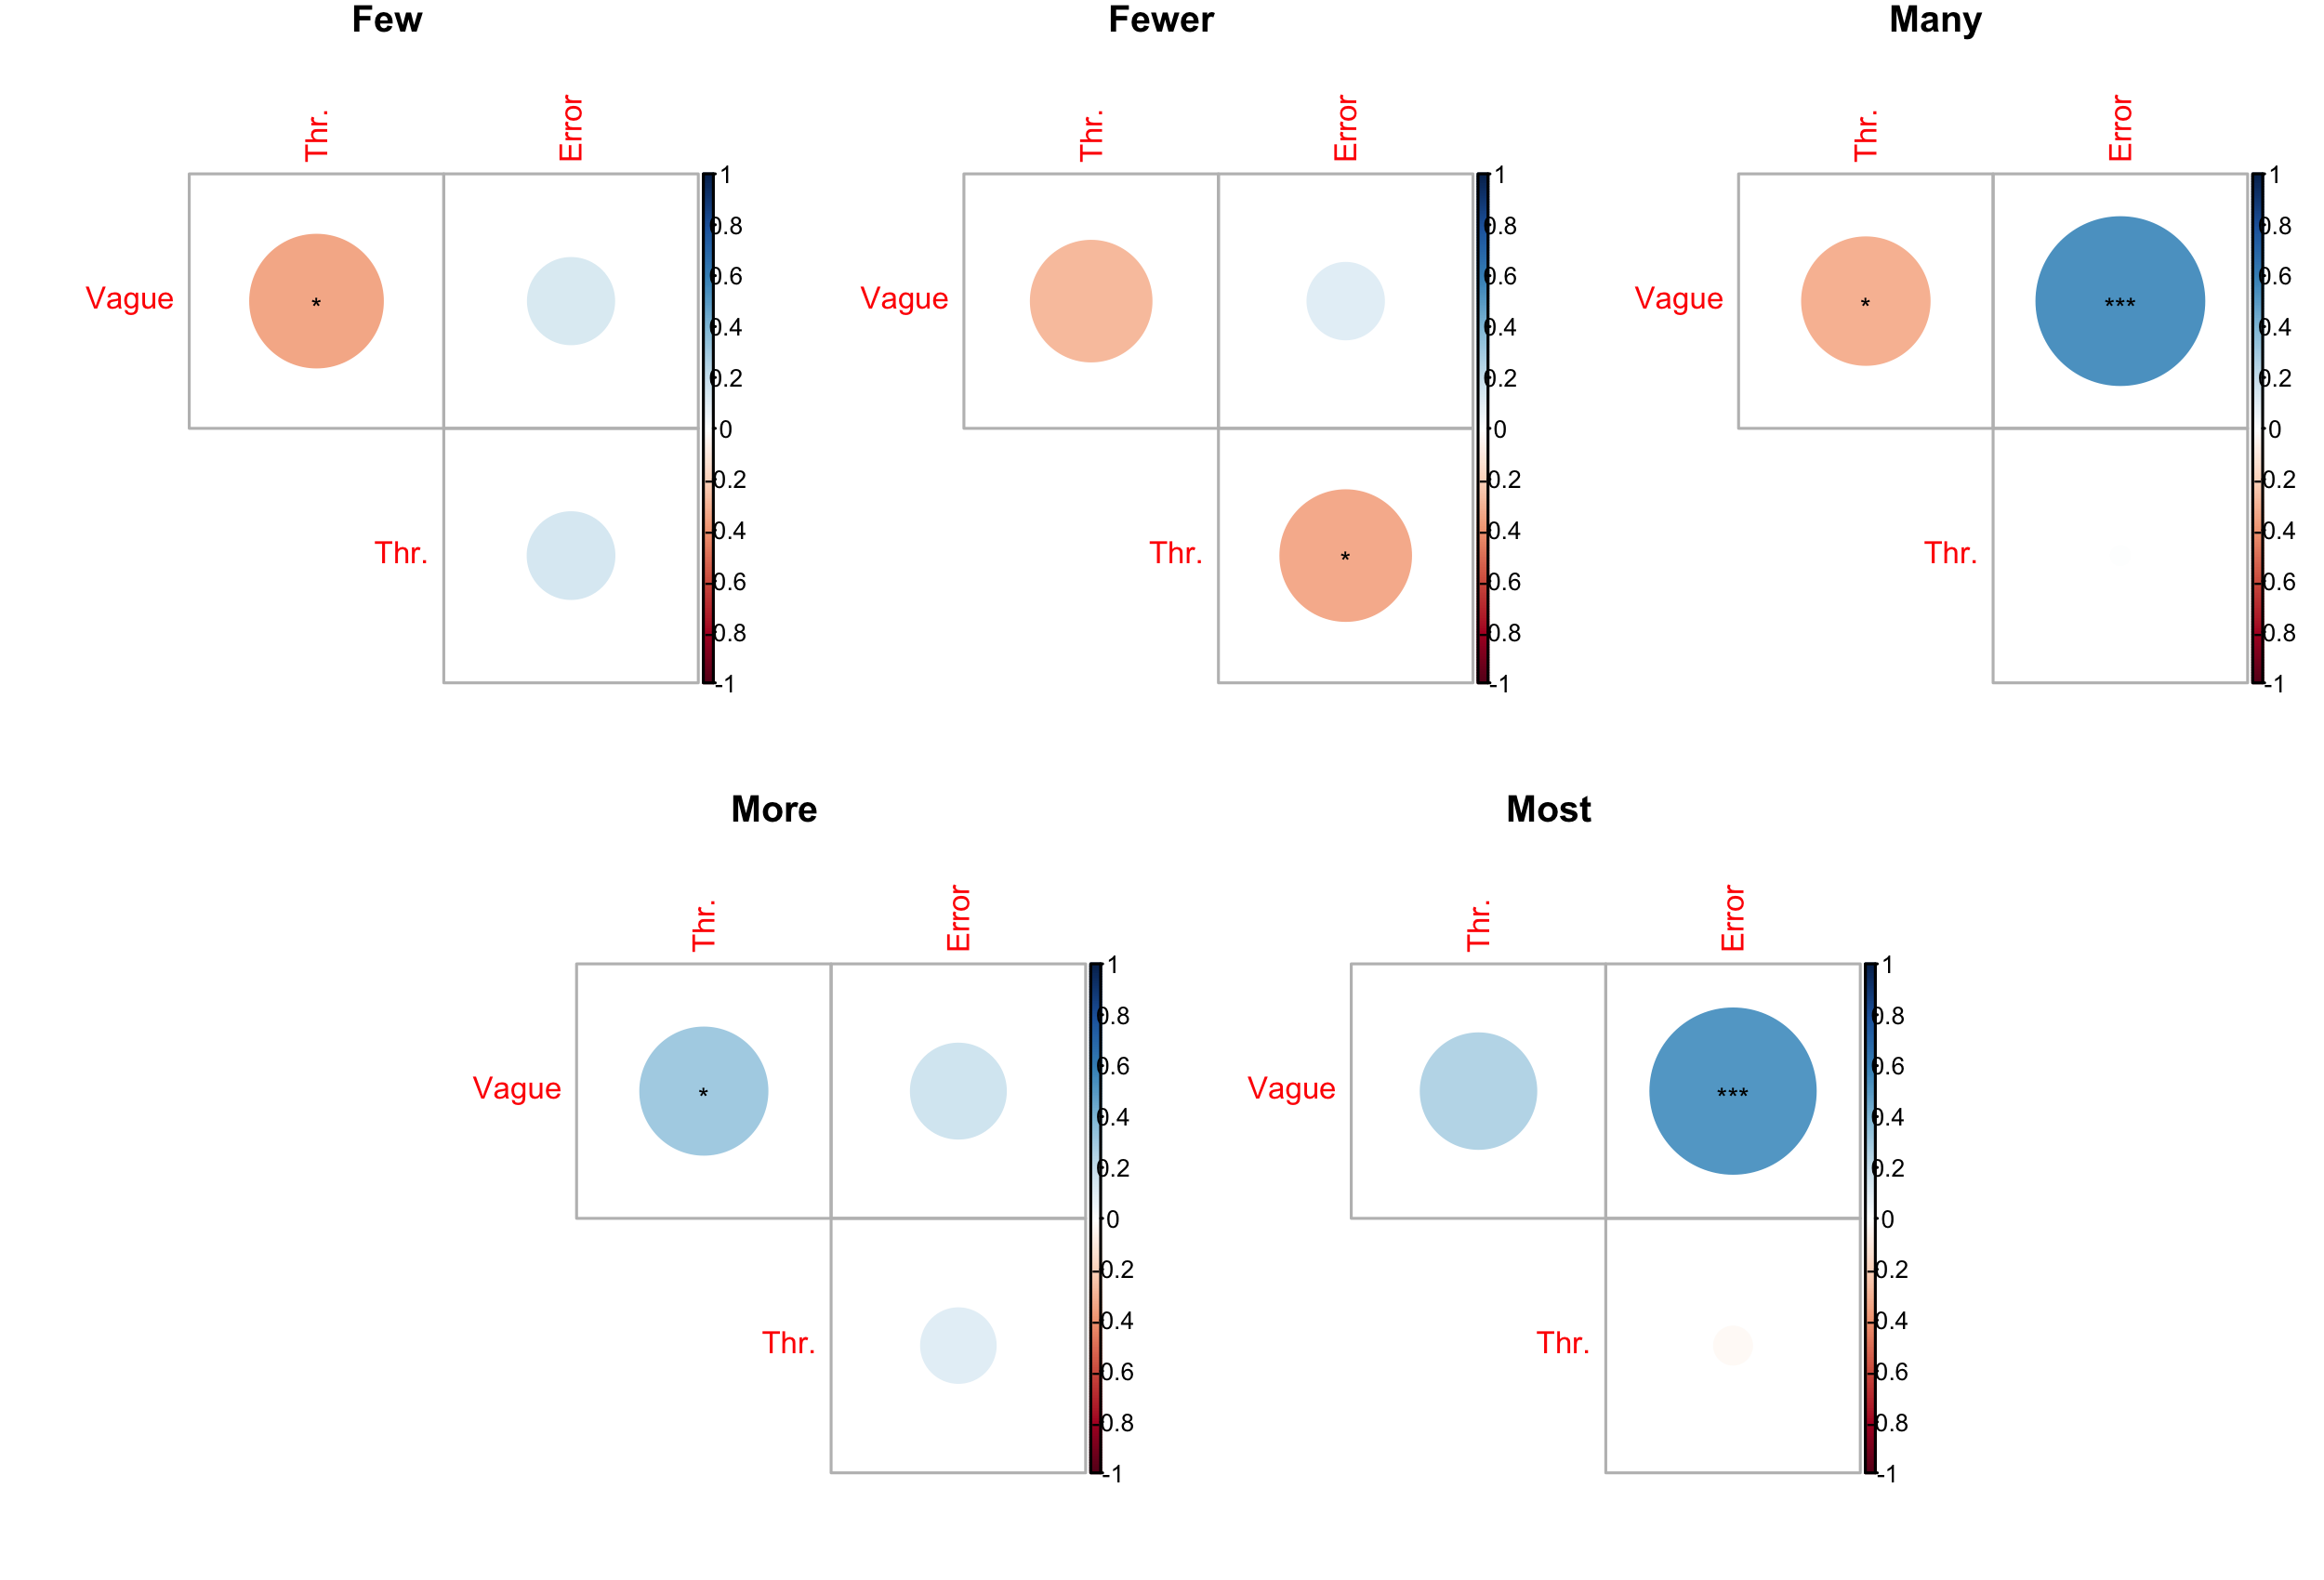
\includegraphics[width=\textwidth]{Figure2.4.png}
    \caption{Correlations of parameters for each quantifier (significance level *** 0.001, ** 0.01, * 0.05). The \textit{p} - values were adjusted using the Bonferroni correction.}
    \label{fig:fig2.4}
\end{figure}

\section{Discussion}
Previous studies showed that quantifiers are organized on a mental scale \cite{Hammerton1976HowPart, Pezzelle2018} and that participants use their internal threshold to verify proportional quantifiers \cite{Shikhare2015ProcessingQuantifiers}. However, little has been known about individual differences in the organization of quantifiers on the mental line. The main goal of this study was to identify subgroups of participants with substantially different meanings of quantifiers. We then investigated whether these subgroups organize quantifiers differently on the mental line. 

First, we examined the correlations between quantifiers for the threshold parameter. This analysis revealed %that participants structure the mental line of quantifiers in a different ways. 
%We found that only the response errors correlated across quantifiers. 
a lack of significant correlations and further motivated the analysis of the subgroups. We ran a cluster analysis on the threshold parameter of each quantifier. We identified three groups of participants with different constellations of thresholds across quantifiers indicating shifts in quantifier meaning. As initially predicted, quantifiers with sharp meaning boundaries, like \textit{fewer than half} and \textit{more than half}, did not contribute to clustering, and they had similar thresholds in all groups. In contrast, thresholds for \textit{many}, \textit{few}, and \textit{most} varied considerably between clusters. In all groups, \textit{most} had the highest threshold. However, the mean threshold varied between clusters. In the first cluster, the mean threshold was 60\%, and in the second and third clusters, the mean thresholds were just slightly above 50\%, at 51\% and 52\%, respectively. For \textit{few}, participants in the first and third clusters had mean thresholds of 35\%, and in the second cluster, the mean threshold was 45\%. The mean threshold for \textit{many} was the most diverse between groups. It ranged from 51\% in the first cluster to 48\% in the second cluster to and 34\% in the third cluster. Together, these results show that individual differences in truth conditions of quantifiers and their position on the mental line are tangible. 

Second, we investigated the order of quantifiers on a mental line. According to the correlation of meaning hypothesis \cite{Douven2019naturalconcepts}, participants may assign different thresholds for the same quantifier, however, they should agree on the order of quantifiers on a mental line. Our results support this hypothesis with the exception that \textit{many} has a more flexible meaning than the other quantifiers.

The third goal of this paper was to look into the relationship between threshold, vagueness, and response error. As predicted, we found that quantifiers with fuzzy meaning boundaries had a higher vagueness value and that negative quantifiers had a higher response error value. We investigated the correlations across parameters for all quantifiers. The lack of systematic patterns in the data supports our modeling choices and justifies usage of the three-parameter model. We will discuss the implications of these findings in more detail in the following subsections.

%Finally, we clustered participants based on vagueness and response error (see Appendix \ref{appendix:ch3}. We found two clusters with high and low vagueness for \textit{many} and two clusters with high and low response error for \textit{few} and \textit{fewer than half}. 

\subsection{The order of quantifiers on the mental line}
Because we failed to find correlations at the group level between thresholds of different quantifiers, we zoomed into the mental line of the subgroups of participants. We observed that the clusters mainly differed in the range of the mental line. %and the order of some quantifiers on it. 
Participants in the first cluster had the most stretched mental line, ranging between 35\% and 60\%, with a clear order of thresholds, where \textit{few} was the lowest and \textit{most} was the highest. In contrast, the second group had the most shrunk mental line, ranging between 45\% and 51\%. The mental scale of the last group stretched between 34\% and 52\%. Moreover, we found that the position of \textit{many} on a mental line was the most flexible and varied substantially between subgroups. 

\citeA{Hammerton1976HowPart} found that although participants assigned different numerical equivalence to quantifiers, they were consistent about the order of the quantifiers. Moreover, according to the correlation of meanings principle \cite{Douven2019naturalconcepts} the between-participants variability in meanings should be constrained by the communication need. Our findings indicate that the order of quantifiers across participants was rather stable, with the exception of \textit{many}. We further discuss the possible explanation of this finding and the relationship between vague quantifier pairs: \textit{few} and \textit{many} (the polar opposites), and \textit{many} and \textit{most}.

\subsubsection{\textit{Many} vs. \textit{few}}
We found an asymmetry between \textit{many} and \textit{few} with regard to their positioning on the mental scale. The position of \textit{many} on the mental scale was more flexible than the position of \textit{few}. In the second and third clusters, the mean threshold for \textit{many} was lower than for \textit{more than half} and \textit{fewer than half}, but in the first cluster, it was higher (see Table \ref{tab:tab2.2} and Figure \ref{fig:fig2.6}). %The second asymmetry between \textit{many} and \textit{few} was that only \textit{many} contributed to clustering based on vagueness.

The flexibility of \textit{many} on the mental scale cannot be explained by its context-dependency. First, in our experiment, we used an artificial context by introducing pseudowords. There was no reason for participants to have different expectations about the context. 
Second, based on the literature \cite{Newstead1987TheScales}, we may predict the opposite pattern of results. The low-magnitude quantifiers, such as \textit{few}, are more context-dependent than high-magnitude quantifiers \cite{Newstead1987TheScales}. Moreover, they can change their threshold depending on the reference set \cite{Newstead1987TheScales} and they are more separated from each other on the mental scale than high-magnitude quantifiers \cite{Pezzelle2018}.

We attribute the asymmetries in our study to competition between quantifiers. While \textit{few} was less than 50\% and \textit{most} was more than 50\% for all clusters, \textit{many} had to compete with both quantifiers for a place on the mental line. As a result of this competition, \textit{many} had a greater variation in threshold and, at least for some participants, was more vague. We observed two tendencies concerning the threshold of \textit{many} (see Figure \ref{fig:fig2.6}). The first tendency was to either keep the threshold for \textit{few} and \textit{many} close together (Clusters 2 and 3) or far apart (Cluster 1). The second tendency was to either keep the threshold for \textit{many} close to \textit{most} (Cluster 2, and to some extent 1) or far from most (Cluster 3, see Figure \ref{fig:fig2.6a}). Despite these tendencies, almost all participants had a higher threshold for \textit{many} than for \textit{few}, and all participants had a higher threshold for \textit{most} than for \textit{many}. Altogether, this finding shows that the position of \textit{many} on the mental line is more flexible than the position of \textit{few} and it explains the membership of the clusters. Nonetheless, in all clusters participants treated \textit{few} as less than \textit{many}, and \textit{many} as less than \textit{most}.

\subsubsection{\textit{Many} vs. \textit{most}}
Previous studies and linguistic analysis \cite{Hackl2009, Pezzelle2018} stressed similarities between \textit{most} and \textit{many}. First, \citeA{Hackl2009} analyzed \textit{most} as a superlative of \textit{many} (\textit{many}+est). This analysis predicts that \textit{most} has to be more than \textit{many}. Our data support this prediction. We showed that not only the mean threshold for \textit{many} was lower than for \textit{most} in all clusters, but also all participants had a higher threshold for \textit{most} than \textit{many} regardless of the cluster's membership (see Figure \ref{fig:fig2.6a}). While all participants treated \textit{most} as the superlative of \textit{many}, the distance between thresholds of these quantifiers was different depending on the cluster. The greatest distance was in the third subgroup.

Second, \citeA{Pezzelle2018} showed substantial overlap in the production of \textit{most} and \textit{many}. Both quantifiers cover comparable proportions on the mental scale. In contrast, our results show individual differences in the distance on the mental line between \textit{most} and \textit{many}. For example, in the third cluster, the mean threshold for \textit{many} was considerably lower than the mean threshold for \textit{most}, while in the second cluster, both thresholds were close to 50\%.

Lastly, \citeA{Pezzelle2018} found that \textit{many} is used less frequently than \textit{most}. We think that the quantifier's vagueness could be one of the sources of the difference in frequency. The high perceived vagueness of \textit{many} lowers its usefulness. The more vague the quantifier, the less information it conveys. However, people try to be as informative as possible \cite{Grice1975} and therefore avoid the usage of uninformative quantifiers with very flexible meanings. This explanation generates a new prediction to test in future work: participants who perceive \textit{many} as vaguer should also use it less often in a production experiment.

\subsection{Relationship between model parameters within quantifiers}
With regard to the relationship between the three model parameters, we did not find a systematic pattern of correlations among quantifiers (see Figure \ref{fig:fig2.4}). The only significant correlation between threshold and response error was for \textit{fewer than half}. This correlation was, however, strongly affected by the outlier participants with a low threshold for \textit{fewer than half} (see Figure \ref{fig:fig2.11} in Appendix \ref{appendix:ch3.4}). Overall, this lack of correlation shows that the variation in thresholds reflects variation in the meaning representations and it is not an artefact of task performance.

We found small to moderate positive correlations between response error and vagueness parameters. As one could expect, the vaguer the quantifier, the more difficult it is to perform the task. However, the correlation was only significant for \textit{many} and \textit{most}. %Moreover, participants from the cluster with higher vagueness for \textit{many} also had a higher response error (Figure \ref{fig:fig2.6}). 
In addition, the lack of systematic correlations between vagueness and response error shows that they correspond to two different processes that should be modeled by separate parameters. %The response error reflects the domain-general cognitive mechanism and related to task difficulty. 
Vagueness thus may correlate with response error for some quantifiers, but it can not be equated with threshold-independent erroneous responding \cite<cf.>{Denic2020Are}. However, the correlation between vagueness and response error was more consistent (at least in direction) than between the other parameters. Relatedly, the overall magnitude of the vagueness parameters was quite small. One reason for both the correlations and the low magnitude might be an issue in identifiability in the model. In the future, it might be helpful to change the parameterization of the model to reduce overlap between the two parameters, for example by modeling asymmetries in vagueness around the threshold.

Finally, we found significant correlations between vagueness and threshold parameters for \textit{many} and \textit{few}, but, importantly, not for \textit{most}. This finding challenges the explanation proposed by \citeA{Solt2016}, according to which participants verify \textit{most} using the approximate strategy \cite{Pietroski2009}. Consequently, the verification of \textit{most} is noisy around 50\%. To reduce the noise, participants prefer thresholds significantly greater than 50\%. This theory predicts that participants with higher thresholds for \textit{most} will perceive it as a vaguer quantifier than participants with lower thresholds. In our model, we captured the noisiness of verification in the vagueness parameter. The lack of significant correlation between vagueness and threshold for \textit{most} does not support Solt's explanation. Instead, it suggests that some participants assigned different truth conditions to \textit{most} and \textit{more than half}.

Overall, the results of the correlation analysis show that each parameter of the model captures a unique aspect of participant performance in the verification task. We interpret this finding as an empirical validation of the assumptions of our model (cf. Figure \ref{fig:fig2.1}).

\subsection{Relationship of model parameters across quantifiers}

We did not find significant correlations across quantifiers for the threshold parameter (see Figure 3), indicating that this parameter was quantifier-specific. In an additional analysis (see Appendix \ref{appendix:ch3}), we tested whether the vagueness and response error parameters are quantifier-specific. Vagueness parameters were not correlated across quantifiers, indicating that similarly to threshold, it is quantifier-specific. In contrast, the response error parameter was significantly correlated across almost all quantifiers. This is in line with our considerations about the model -- response error reflects cognitive abilities independent of the quantifiers, while vagueness contains information about quantifier meaning.

The correlations for the response error parameters were stronger between negative than positive quantifiers because of the greater variation in response error in negative quantifiers. Due to this variation, only negative quantifiers contributed to the clustering on response error. Response error, thus, reflects a combination of general task performance ability and specific difficulty in verification for negative quantifiers \cite{Deschamps2015ThePerception., Just1971ComprehensionQuantification, Schlotterbeck2020RepresentationalEffect}. We noted that the cluster with a higher rate of response error was small (\textit{N} = 7), probably because the task was generally easy. It would be worth testing whether the response error parameter contributes more to clustering in a more challenging task, for example, with visual displays instead of sentences.

\subsection{Sources of individual differences}
Our starting point for the investigation of individual differences in meaning representations of natural language quantifiers was the observation that language users can have different truth conditions for logical words \cite<e.g.,>{Yildirim2016}. For example, previous studies \cite<e.g.,>{Spychalska2016InvestigatingPotentials} showed that two groups of speakers have different interpretations of the quantifier \textit{some}. In this spirit, we demonstrated that this phenomenon is not limited to just one quantifier. We showed that there are three subgroups of participants with different thresholds for \textit{many}, \textit{few}, and \textit{most}.

The question remains, however, how individual differences in thresholds emerge. We consider here a few possible explanations. First, we argue that individual differences are not due to the various verification strategies used by participants \cite<cf.,>{Talmina2017}. We think that this explanation is unlikely because the task design limited possible strategy choices. Participants verified the sentence with a quantifier by comparing their threshold to the proportion given as a number. Although the Approximate Number System \cite{Dehaene1997TheMathematics} could have interfered with the precise number system, it is rather unlikely that participants were unable to precisely compare proportions. In our task, there was no time pressure on the decision and the proportions were displayed on the screen for an unlimited period of time. We feel confident in rejecting the explanations based on the variability in verification strategies as a source of observed individual differences in thresholds in our study.

The individual differences in thresholds are also unlikely to be a result of the different cognitive abilities of our participants \cite<e.g.,>{Just1992AMemory, Steinert-Threlkeld2015, Zajenkowski2014WorkingVerification}. We did not measure the working memory or executive function performance of participants, but our task was relatively easy and did not require much working memory or other cognitive function resources. Moreover, we included a response error parameter in our model, which accounted for variability in task performance (e.g., attention lapses or mistakes). We found that the majority of participants belonged to a low response error cluster (see Appendix \ref{appendix:ch3.3}), indicating that they performed the task at a similar level of accuracy. Altogether, we conclude that the differences in thresholds between groups are due to different representations of the truth conditions of quantifiers.

Another possible explanation of individual differences in thresholds arises from studies on informativeness and pragmatic abilities. For example, \citeA{Nieuwland2010OnAbilities} showed using the electroencephalography marker of semantic processing that participants with better pragmatic abilities are more sensitive to underinformative sentences compared to less skilled participants. According to this line of argumentation, participants in our study had the same meaning representations of quantifiers. The observed individual differences in thresholds thus are driven by a pragmatic mechanism.

While we can not rule out the pragmatic explanation of our result, we would like to point out some challenges to this interpretation. First, previous studies investigating the role of pragmatic abilities in the interpretation of underinformative sentences are inconclusive \cite<cf.,>{Nieuwland2010OnAbilities, Spychalska2016InvestigatingPotentials}. Some studies \cite<e.g.,>{Spychalska2016InvestigatingPotentials} did not find a correlation between pragmatic skills and sensitivity to underinformativeness. Secondly, it is difficult to provide a single pragmatic mechanism that would explain individual differences in thresholds of all quantifiers. For example, it has been argued that the higher threshold for \textit{most} compared to \textit{more than half} is a result of pragmatic strengthening \cite{Solt2016}. Recent studies \cite{Denic2020Are} tested this prediction directly and challenged the pragmatic strengthening hypothesis. Moreover, the mechanism of pragmatic strengthening can not explain the individual differences in thresholds of \textit{many} and \textit{few}. The variability in thresholds for \textit{many} and \textit{few} is often explained by different expectations related to the contextual factors \cite<e.g.,>{Fernando1996ExpectingMany}. However, in our study, the contextual information was fairly abstract and unlikely to elicit specific expectations. More research is needed to fully understand the complexity of the semantics-pragmatics interface and its effect on the structure of the quantifier mental line.

Finally, the individual differences may have emerged due to participants being sensitive to different pressures that shape the space of meanings. \citeA{Douven2019naturalconcepts} put forward the idea that the space of natural concepts is optimally designed, meaning that it satisfies design criteria and constraints \cite<see also>[for discussion]{Douven2019Rationality}. For example, the space of concepts should be informative but also parsimonious and learnable. Analogue criteria could be applied to the quantifier mental line. We suggest that the subgroups may differ in which criteria shape their space of meanings primarily, and as a result, they could apply different thresholds. Further studies would be needed to test this hypothesis. Moreover, future research should investigate how participants belonging to different clusters can communicate with each other. The adjustment of the threshold between participants called the semantic adaptation \cite<e.g.,>{Schuster2019adaptationuncertaintyexpressions} is one of the possible mechanisms. Further studies should investigate the role of vagueness in semantic adaptation. The fuzziness around the threshold may facilitate the ``meeting of minds" \cite{Douven2019naturalconcepts} by leaving space for shifting the thresholds. %However, the change in the threshold would require reorganization of quantifier mental line \cite<cf.,>{Heim2015Ifmany}, which may be potentially cognitively costly. Another possibility is that vagueness constitute the bridge for the ``meeting of minds" \cite{Douven2019naturalconcepts}. By allowing for fuzziness around the thresholds participants can align the meanings without reorganizing the whole quantifier mental line.

\subsection{Conclusions}
In the current study, we separated individual differences in meaning representations, such as vagueness and threshold, from general cognitive abilities reflected in a response error parameter using a Bayesian modeling approach. Based on the model's threshold parameters, we identified three clusters of participants assigning different meanings to vague quantifiers such as \textit{most}, \textit{many}, and \textit{few}. We showed that these quantifiers have different positions on the mental scale in subgroups of participants. Our findings are consistent with the claim that logical words can have various semantic representations for different speakers. We believe that our approach could be helpful for studying individual differences in the representation of not only quantifiers but also other functional or content words. In sum, in this paper, we showed that our computational model can bring together formal semantic and psycholinguistic approaches to study meaning representations.

\section{Acknowledgements}
This work was supported by the European Research Council under the European Union's Seventh Framework Programme (FP/2007–2013)/ERC Grant Agreement n.STG 716230 CoSaQ. 

\bibliographystyle{apacite}
\bibliography{references_v4.bib}

\appendix
\section{Appendix}\label{appendix:ch3}
\subsection{Correlations of vagueness and response error parameters across quantifiers}\label{appendix:ch3.1}
Figure \ref{fig:fig2.3b} shows the correlations for vagueness, and Figure \ref{fig:fig2.3c} for response errors. The correlations for vagueness were weak, suggesting that this parameter is quantifier-specific and not domain-general. In contrast, the correlations for response error varied, ranging from a strong correlation between \textit{few} and \textit{fewer than half} (\textit{r} = 0.75), to the weakest correlation between \textit{more than half} and \textit{many} (\textit{r} = 0.24, see Figure \ref{fig:fig2.3c}). The strongest correlation was significantly higher than the weakest, Steiger's test \textit{z} = 4.72, \textit{p} $< 0.001$. This suggests that response error reflects general cognitive ability.

\begin{figure} [H]
\begin{minipage}[b]{0.49\textwidth}
    \begin{subfigure}[b]{\linewidth}
     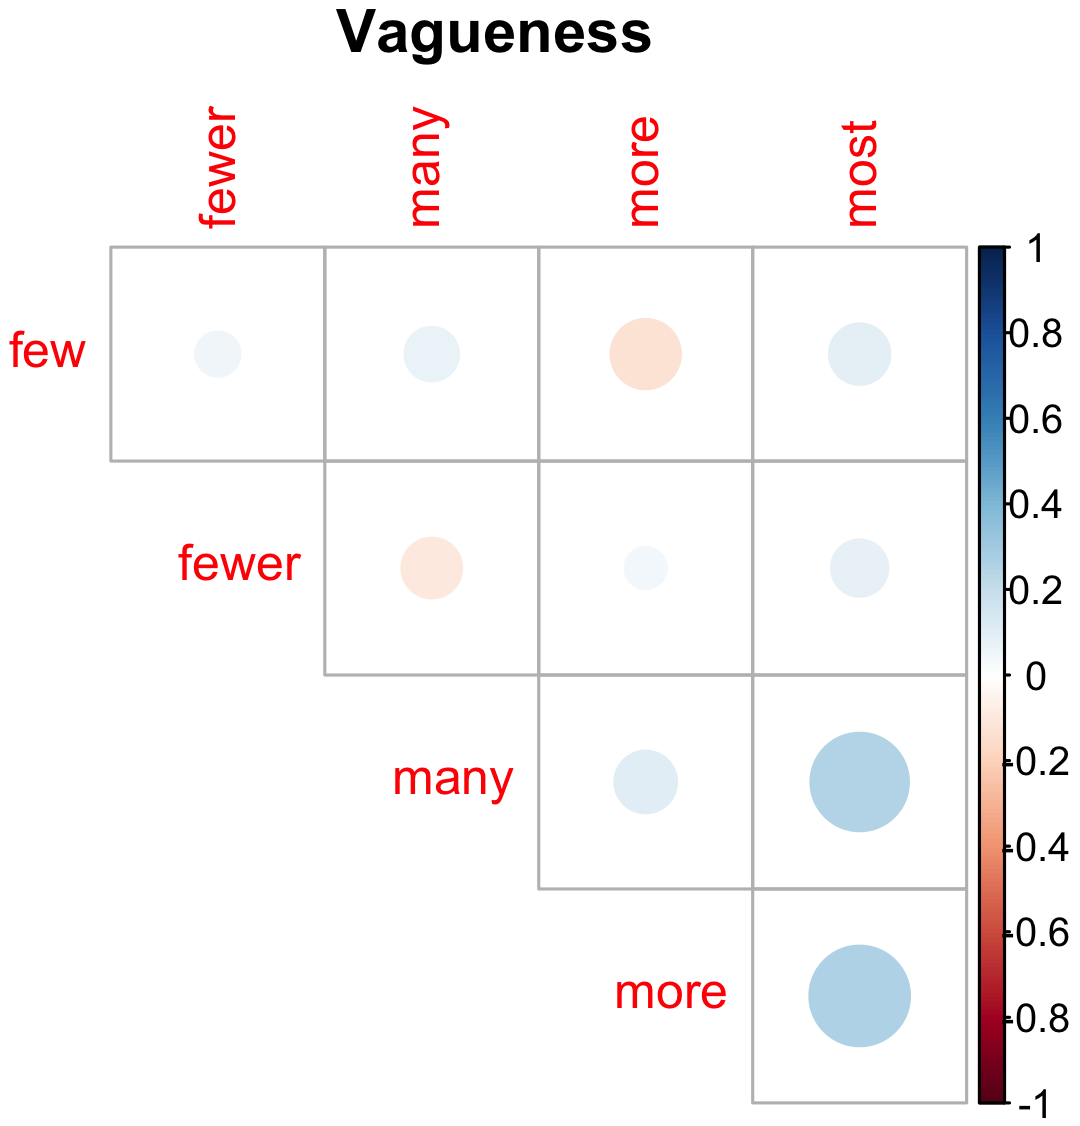
\includegraphics[width=\linewidth]{Figure2.3b.png}
     \caption{\label{fig:fig2.3b}}
    \end{subfigure}
\end{minipage}    
\hfill
\begin{minipage}[b]{0.49\textwidth}
    \begin{subfigure}[b]{\linewidth}
     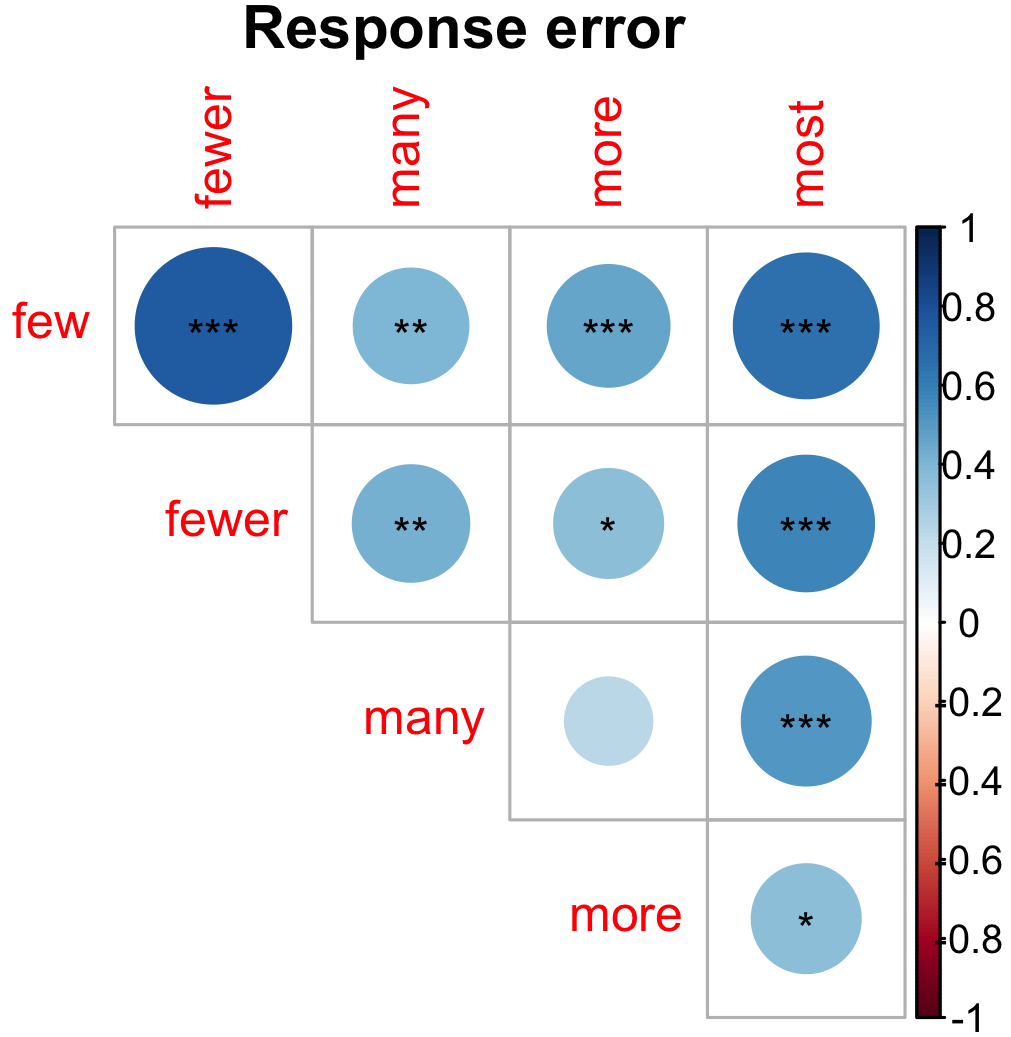
\includegraphics[width=\linewidth]{Figure2.3c.png}
     \caption{\label{fig:fig2.3c}}
    \end{subfigure}
\end{minipage}
    \caption{\ref{fig:fig2.3b} correlations between vagueness; \ref{fig:fig2.3c} correlations between response error (significance level *** 0.001, ** 0.01,*  0.05). The \textit{p} - values were adjusted using the Bonferroni correction.}
    \label{fig:fig2.3app}
\end{figure}


\subsection{Vagueness}\label{appendix:ch3.2}
\subsubsection{Cluster analysis}
We expected polar opposite quantifiers \textit{few} and \textit{many} to make comparable contributions to clustering on vagueness. What we observed instead was the asymmetry in \textit{many} and \textit{few}. The elbow plot and Silhouette method agreed that the two-cluster solution was optimal, identifying one cluster (\textit{N} = 24) with high vagueness for \textit{many}, and a second cluster (\textit{N} = 47) with lower vagueness for \textit{many} (Table \ref{tab:tab2.3}). %Figure \ref{fig:fig2.7} shows that participants with higher vagueness for \textit{many} had a tendency to make more mistakes and had lower threshold, while participants with lower vagueness for \textit{many} had a threshold concentrated around 50\% and made fewer errors.

\iffalse
\begin{figure} [H]
    \centering
    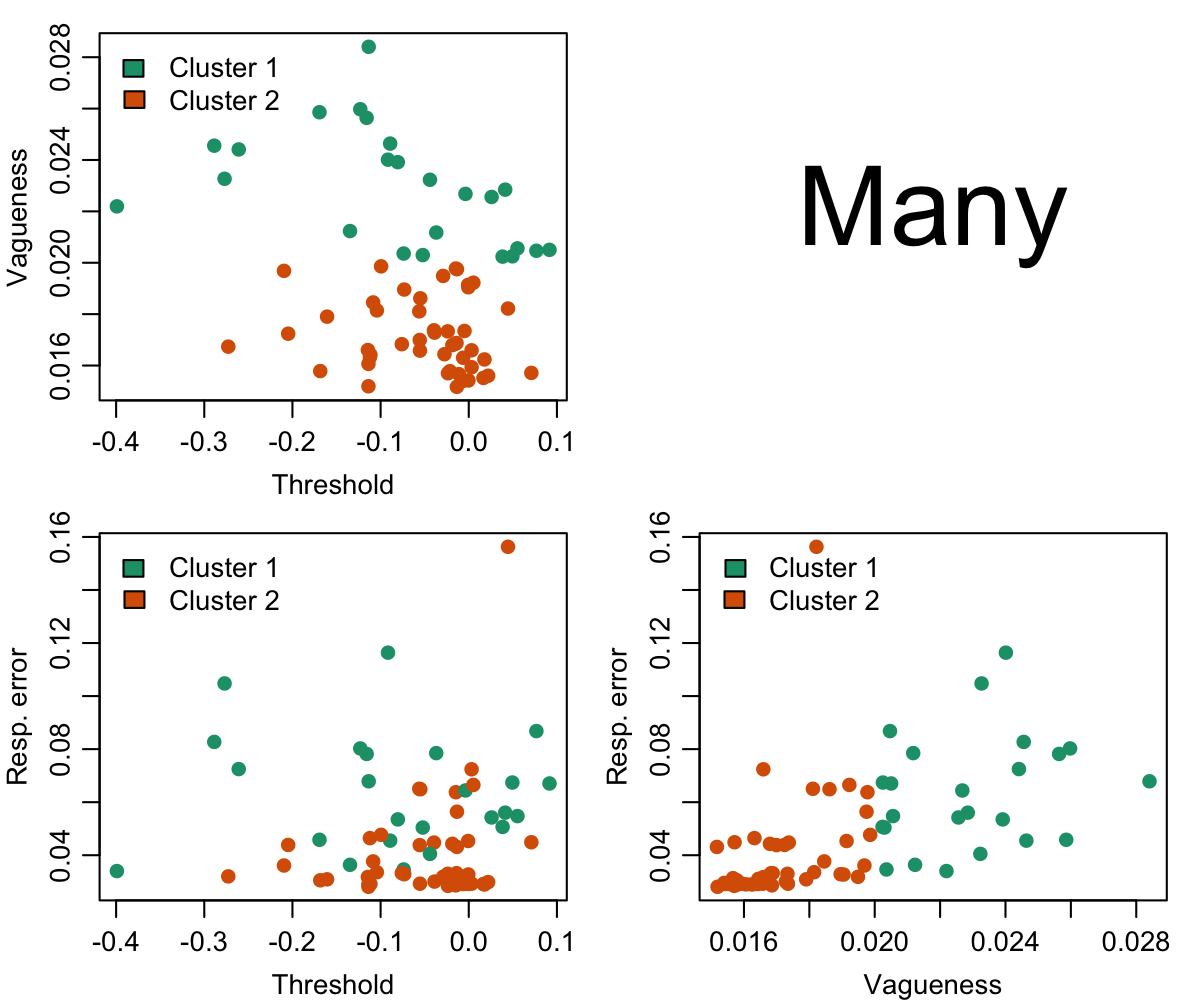
\includegraphics[width=\textwidth]{Figure2.7.png}
    \caption{Relationship between threshold, vagueness, and response error for \textit{many}, indicating two clusters based on vagueness. Cluster 1 (\textit{N} = 24) with higher vagueness for \textit{many} is indicated in green, and Cluster 2 (\textit{N} = 47) with lower vagueness for \textit{many} in orange.}
    \label{fig:fig2.7}
\end{figure}
\fi

\begin{table}[H]
    \centering
    \caption{Mean (\textit{SD}) vagueness parameter in each cluster, 2-cluster solution. }
    \label{tab:tab2.3}
    \begin{tabular}{lcccc}\hline
         Quantifier & Cluster 1 & Cluster 2 \\
          & (\textit{N} = 24) & (\textit{N} = 47) \\
         \hline
         \textit{Few} & .016 (.001) & .016 (.001)\\
         \textit{Fewer than half} & .002 (.00004) & .002 (.00004)\\
         \textit{Many} & .023 (.002) & .017 (.001)\\
         \textit{More than half} & .001 (.00004) & .001 (.00002)\\
         \textit{Most} & .009 (.001) & .009 (.001)\\ \hline
    \end{tabular}
\end{table}

\subsubsection{Linear Discriminant Analysis}
For the vagueness parameter, we expected vague quantifiers to contribute to the clustering. We found that only \textit{many} contributed significantly to the clustering ($\lambda$ = 0.29, \textit{p} $<$ 0.001). The LDA achieved 94\% accuracy in classification of participants into clusters based on vagueness parameters for \textit{many}, and the leave-one-out cross validation accuracy was 94\%.

\subsection{Response error}\label{appendix:ch3.3}
\subsubsection{Cluster analysis}
The elbow plot suggested that either two or three clusters should be optimal, but the Silhouette method indicated the 2-cluster solution. Assuming two clusters, we found a cluster of participants with few response errors (\textit{N} = 64) and a cluster with more response errors (\textit{N} = 7) across quantifiers, see Table \ref{tab:tab2.4}. This means that the majority of participants had a low response error rate. The difference in response error between clusters was most prominent for negative quantifiers. %Figure \ref{fig:fig2.8} shows the relationship between model parameters based on response error clustering for \textit{few} and \textit{fewer than half}. For \textit{few}, we did not observe that participants with a high response error had a tendency toward more extreme thresholds or vagueness, while for \textit{fewer than half} some participants that made more errors also had lower threshold. 

\begin{table}[H]
    \centering
    \caption{Mean (\textit{SD}) response error parameter in each cluster, 2-cluster solution.}
    \label{tab:tab2.4}
    \begin{tabular}{lcccc}\hline
        Quantifier & Cluster 1 & Cluster 2 \\
        & (\textit{N} = 7) & (\textit{N} = 64) \\ \hline
         \textit{Few} & .17 (.05) & .05 (.02)\\
         \textit{Fewer than half} & .19 (.03) & .06 (.03)\\
         \textit{Many} & .08 (.04) & .05 (.02)\\
         \textit{More than half} & .06 (.02) & .04 (.02)\\
         \textit{Most} & .09 (.03) & .04 (.02)\\ \hline
    \end{tabular}
\end{table}

\iffalse
\begin{figure} [H]
    \begin{minipage}[b]{0.45\textwidth}
    \begin{subfigure}[b]{\linewidth}
     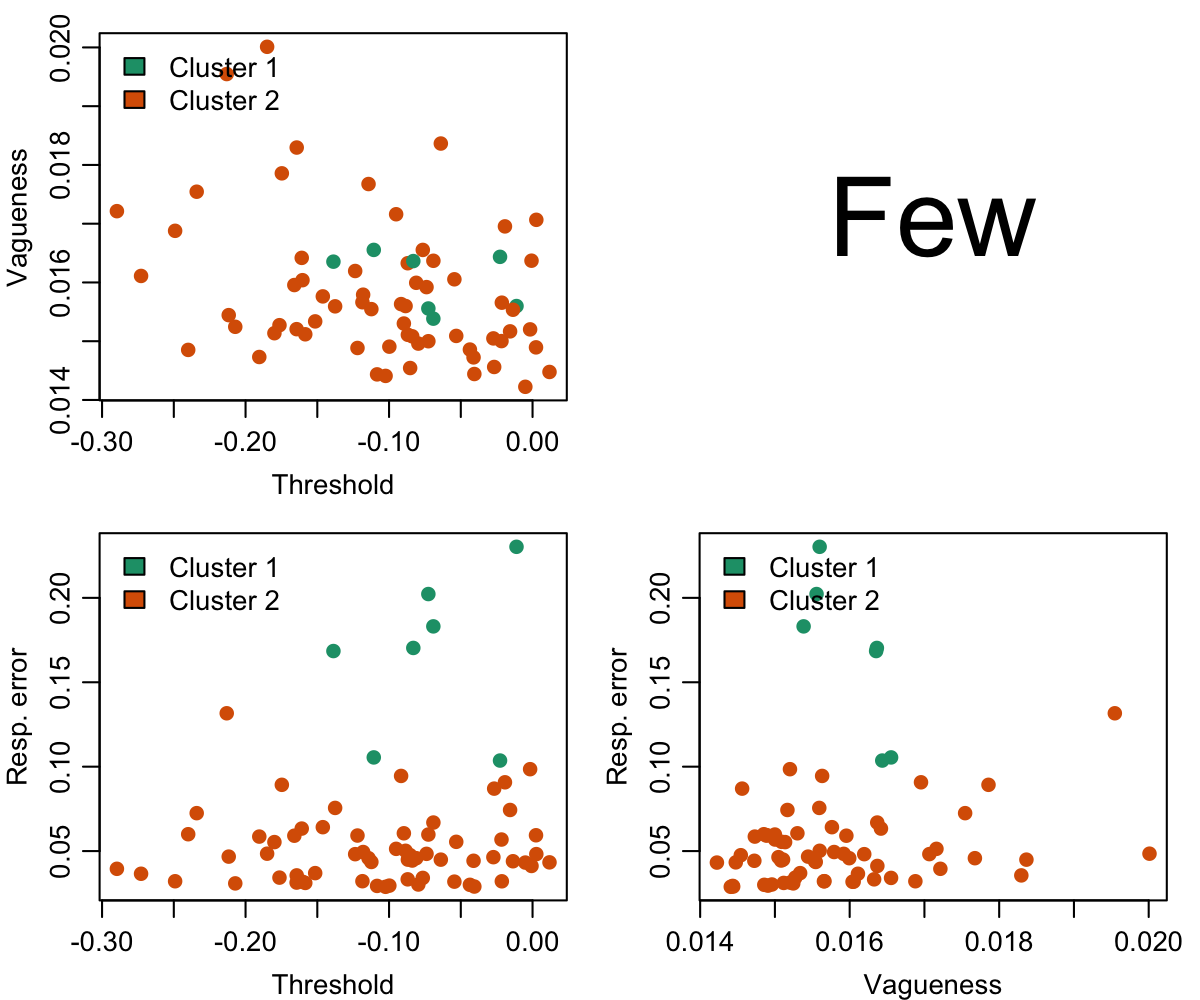
\includegraphics[width=\linewidth]{Figure2.8a.png}
     \caption{\label{fig:fig2.8a}}
    \end{subfigure}
    \end{minipage}
    \hfill
    \begin{minipage}[b]{0.45\textwidth}
    \begin{subfigure}[b]{\linewidth}
     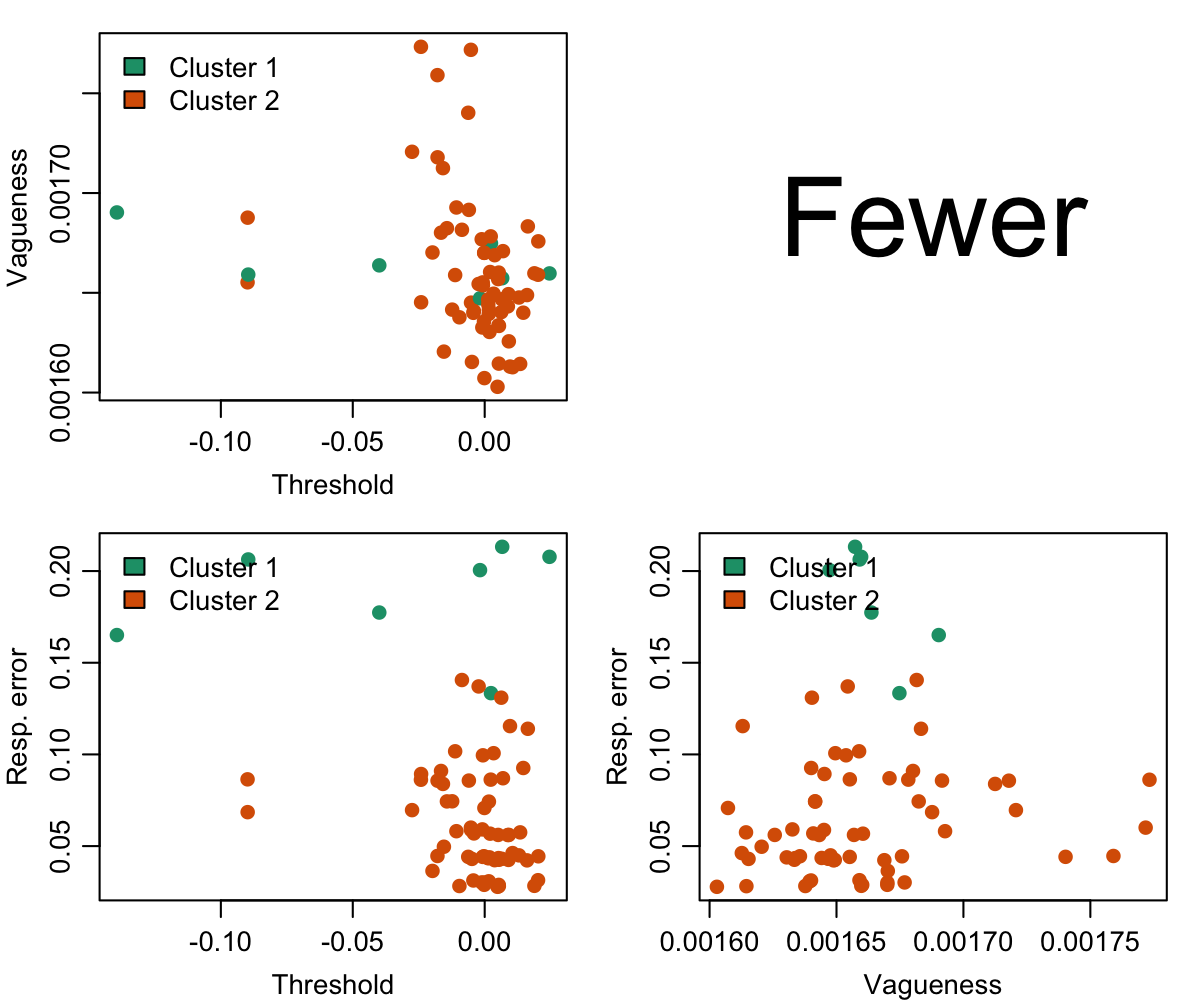
\includegraphics[width=\linewidth]{Figure2.8b.png}
     \caption{\label{fig:fig2.8b}}
    \end{subfigure}
    \end{minipage}
    \caption{Relationship between threshold, vagueness, and response error for \textit{few} (\ref{fig:fig2.8a}) and \textit{fewer than half} (\ref{fig:fig2.8b}), indicating two clusters based on response error. Cluster 1 (\textit{N} = 7) with a high response error is indicated in green, and Cluster 2 (\textit{N} = 64) with a lower response error in orange.}
    \label{fig:fig2.8}
\end{figure}
\fi

\subsubsection{Linear Discriminant Analysis}
We expected the response error parameter for negative quantifiers to contribute more to clustering. In line with this hypothesis, the Wilks test showed a significant contribution of response error parameters for \textit{few} ($\lambda$ = 0.32, \textit{p} $<$ 0.001) and \textit{fewer than half} ($\lambda$ = 0.25, \textit{p} $<$ 0.001), but not for \textit{many}, \textit{most} and \textit{more than half}. Figure \ref{fig:fig2.10} shows the combined effect of the two quantifiers on clustering. Participants who made more errors while verifying \textit{few} also made more errors for \textit{fewer than half}. We used the LDA to predict the cluster membership for each participant based on response error parameters for \textit{few} and \textit{fewer than half}. The LDA achieved 99\% accuracy, and the leave-one-out cross validation accuracy was 99\%.

\begin{figure} [H]
    \centering
    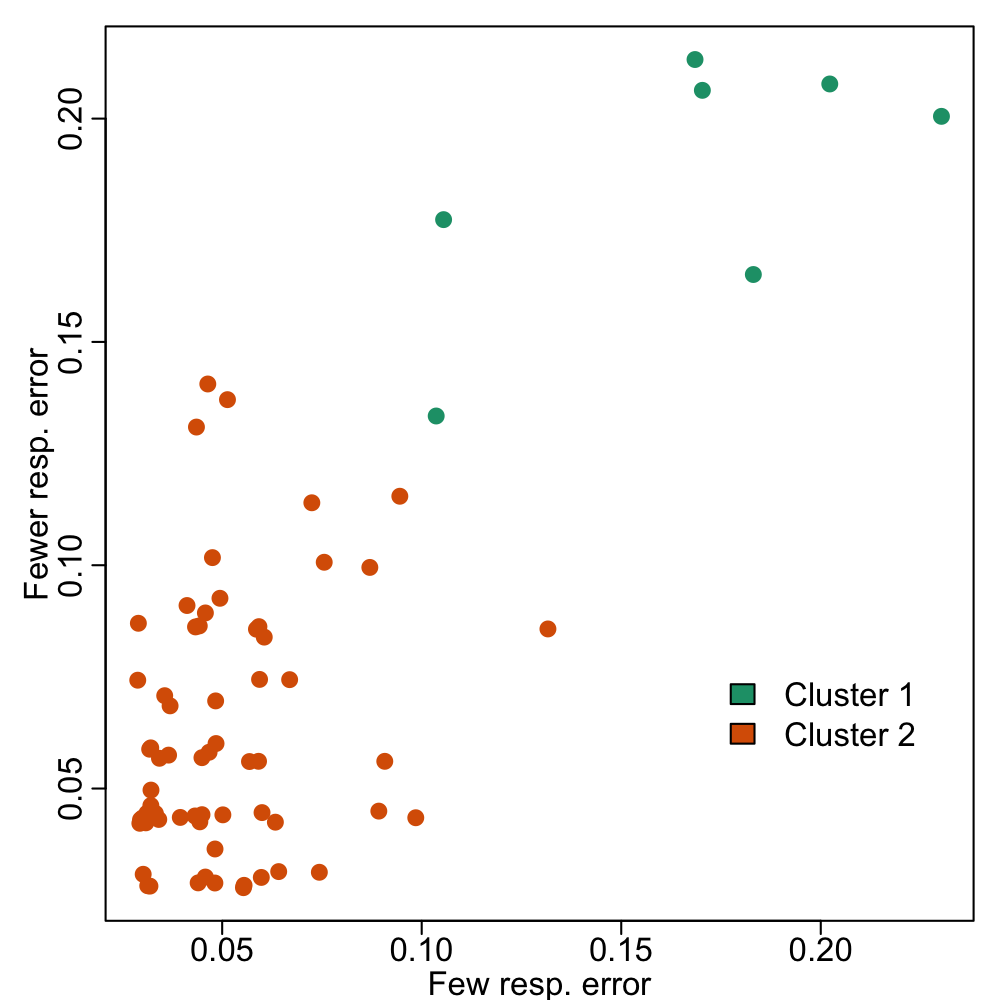
\includegraphics[scale=0.2]{Figure2.10.png}
    \caption{Two clusters for response error based on \textit{few} and \textit{fewer than half} parameters. The response error values of parameters for \textit{fewer than half} are plotted against the response error values for \textit{few}. Colors are used to indicate the cluster membership: Cluster 1 (\textit{N} = 7) with high response error is in indicated in green, and Cluster 2 (\textit{N} = 64) with low response error in orange.}
    \label{fig:fig2.10}
\end{figure}

\subsection{Influential observations}\label{appendix:ch3.4}
Figure 11 illustrates how relationships between model parameters for each quantifier are affected by influential observations. We computed the Cook’s distance using the \textit{ols plot cooksd bar} R function in the package \textit{olsrr} \cite{Hebbali2020Tools0.5.3}.

\begin{figure} [H]
   \begin{minipage}[b]{0.49\textwidth}
    
    \begin{subfigure}[b]{\linewidth}
   % \centering
     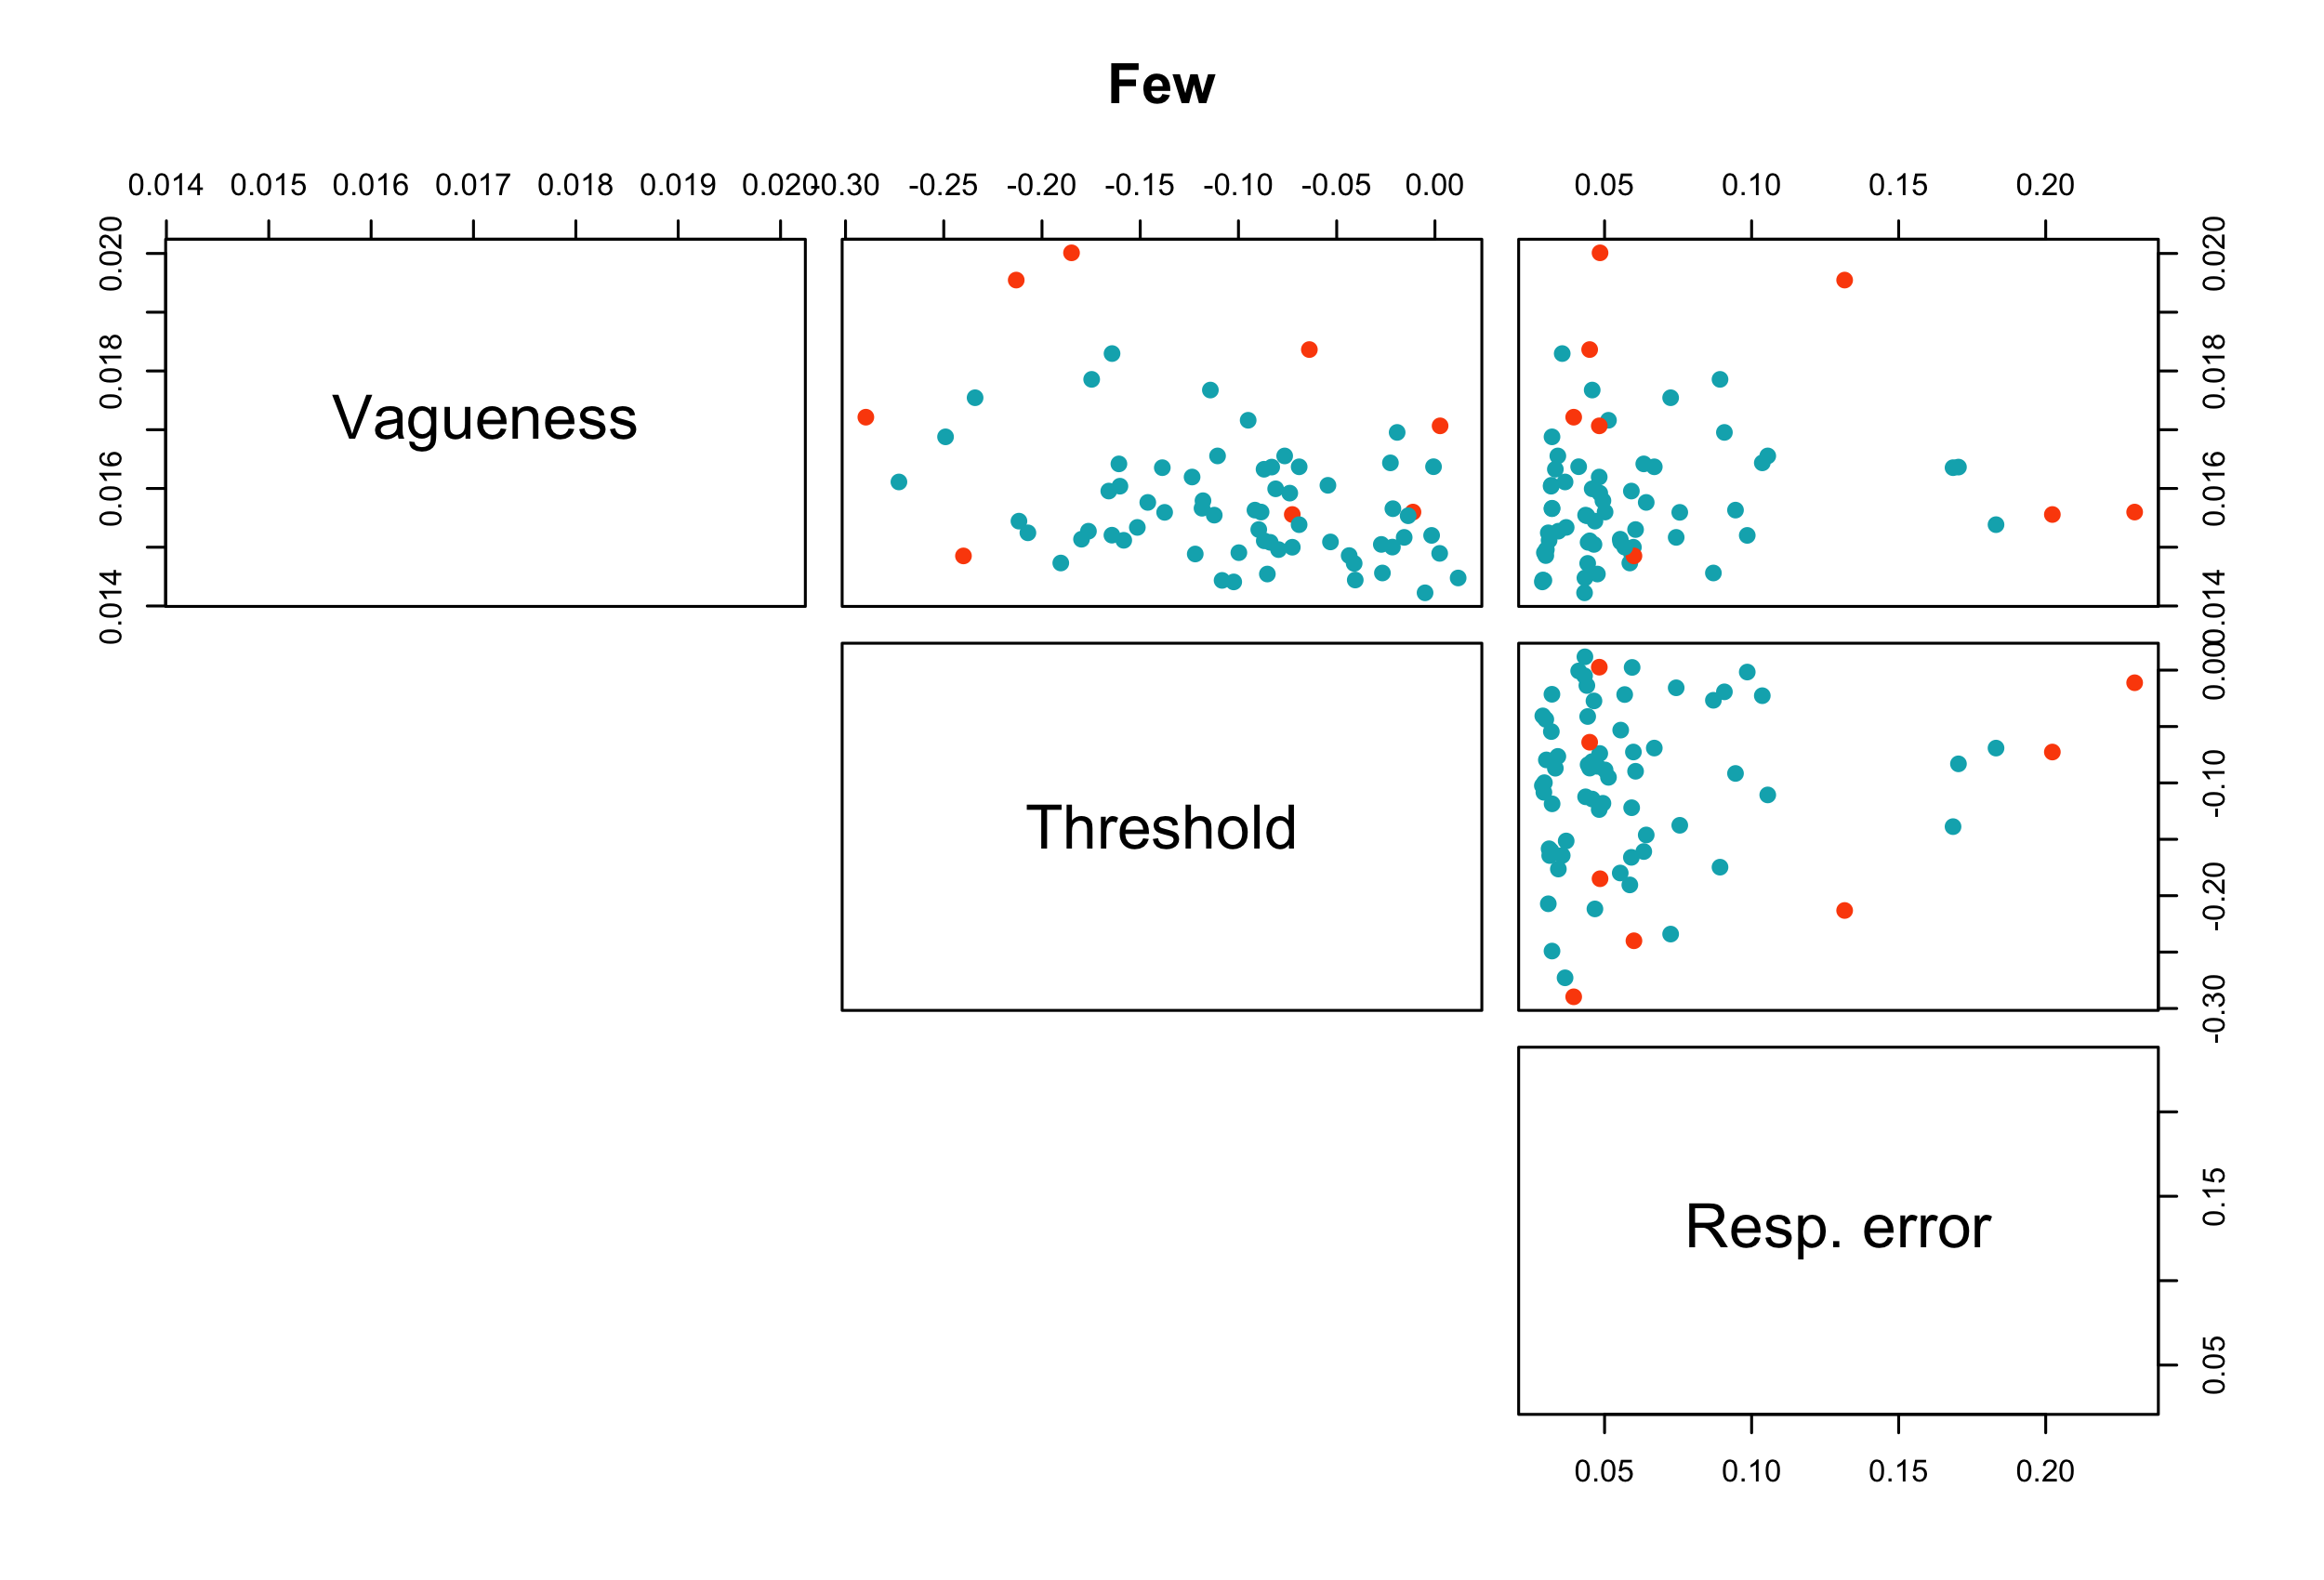
\includegraphics[width=\linewidth]{Figure2.11a.png}
     \caption{\label{fig:fig2.11a}}
    \end{subfigure}
    
    \vspace*{4mm}
    \begin{subfigure}[b]{\linewidth}
     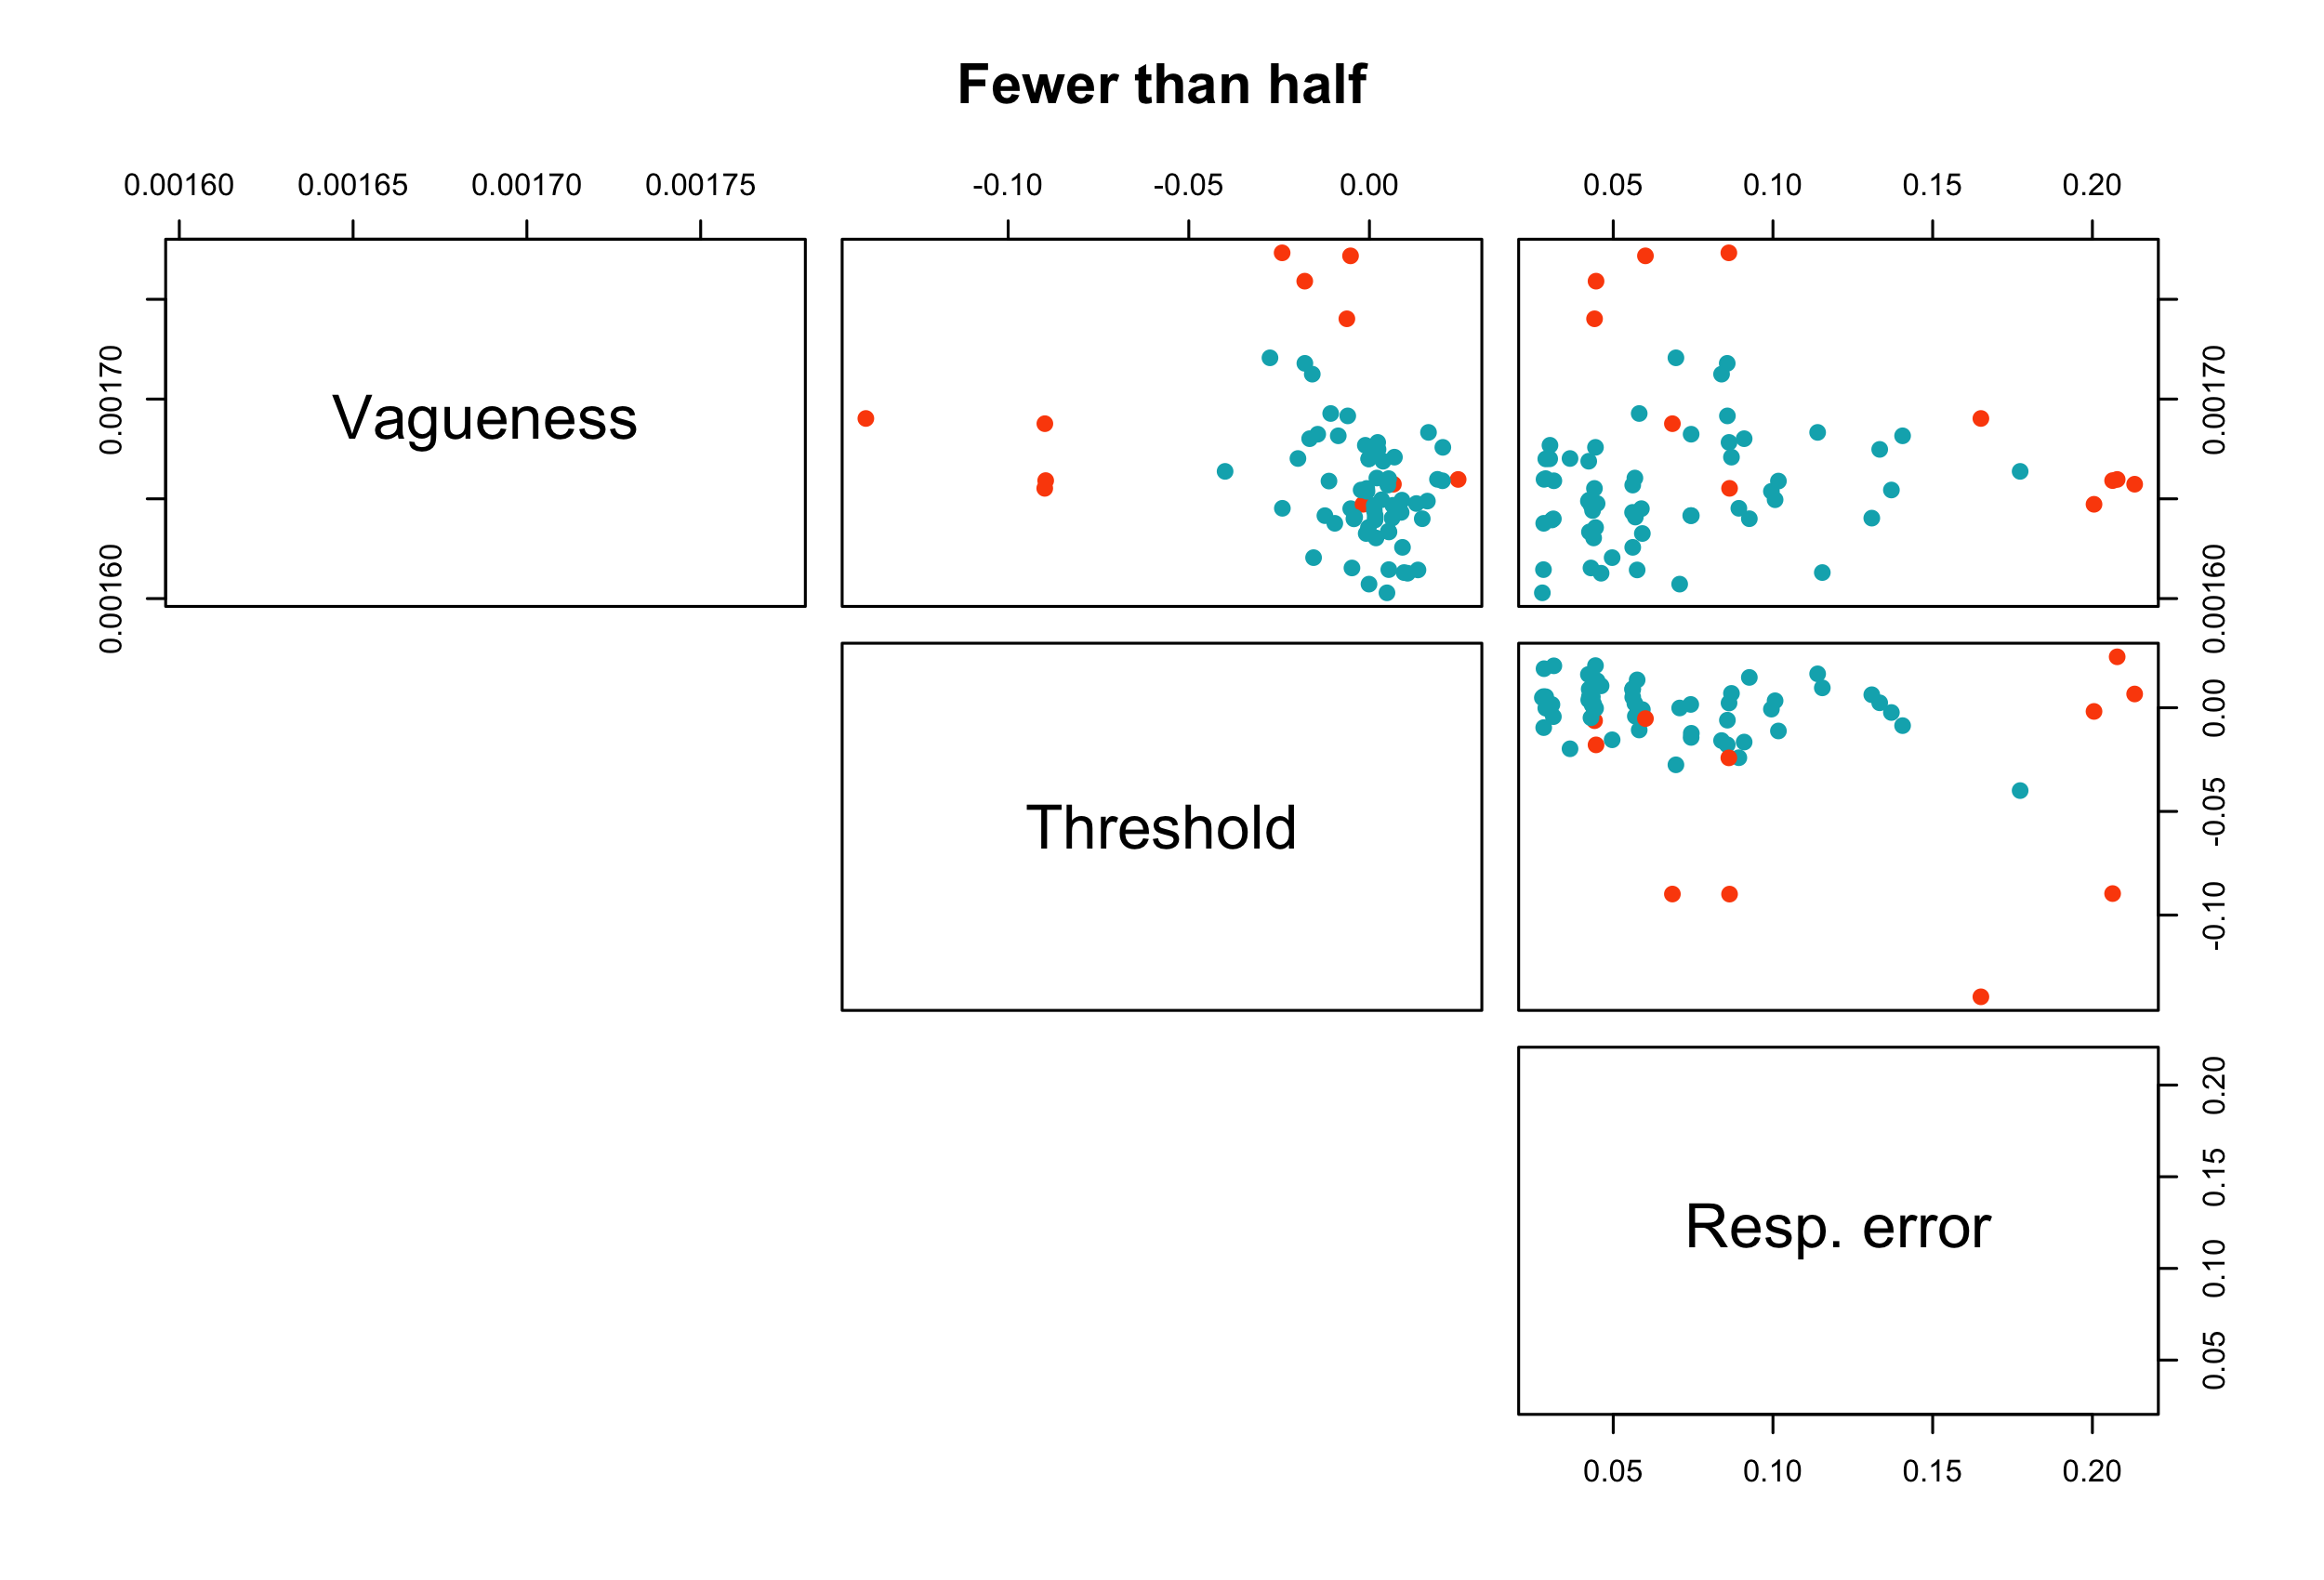
\includegraphics[width=\linewidth]{Figure2.11b.png}
     \caption{\label{fig:fig2.11b}}
    \end{subfigure}
    
    \vspace*{4mm}
    \begin{subfigure}[b]{\linewidth}
     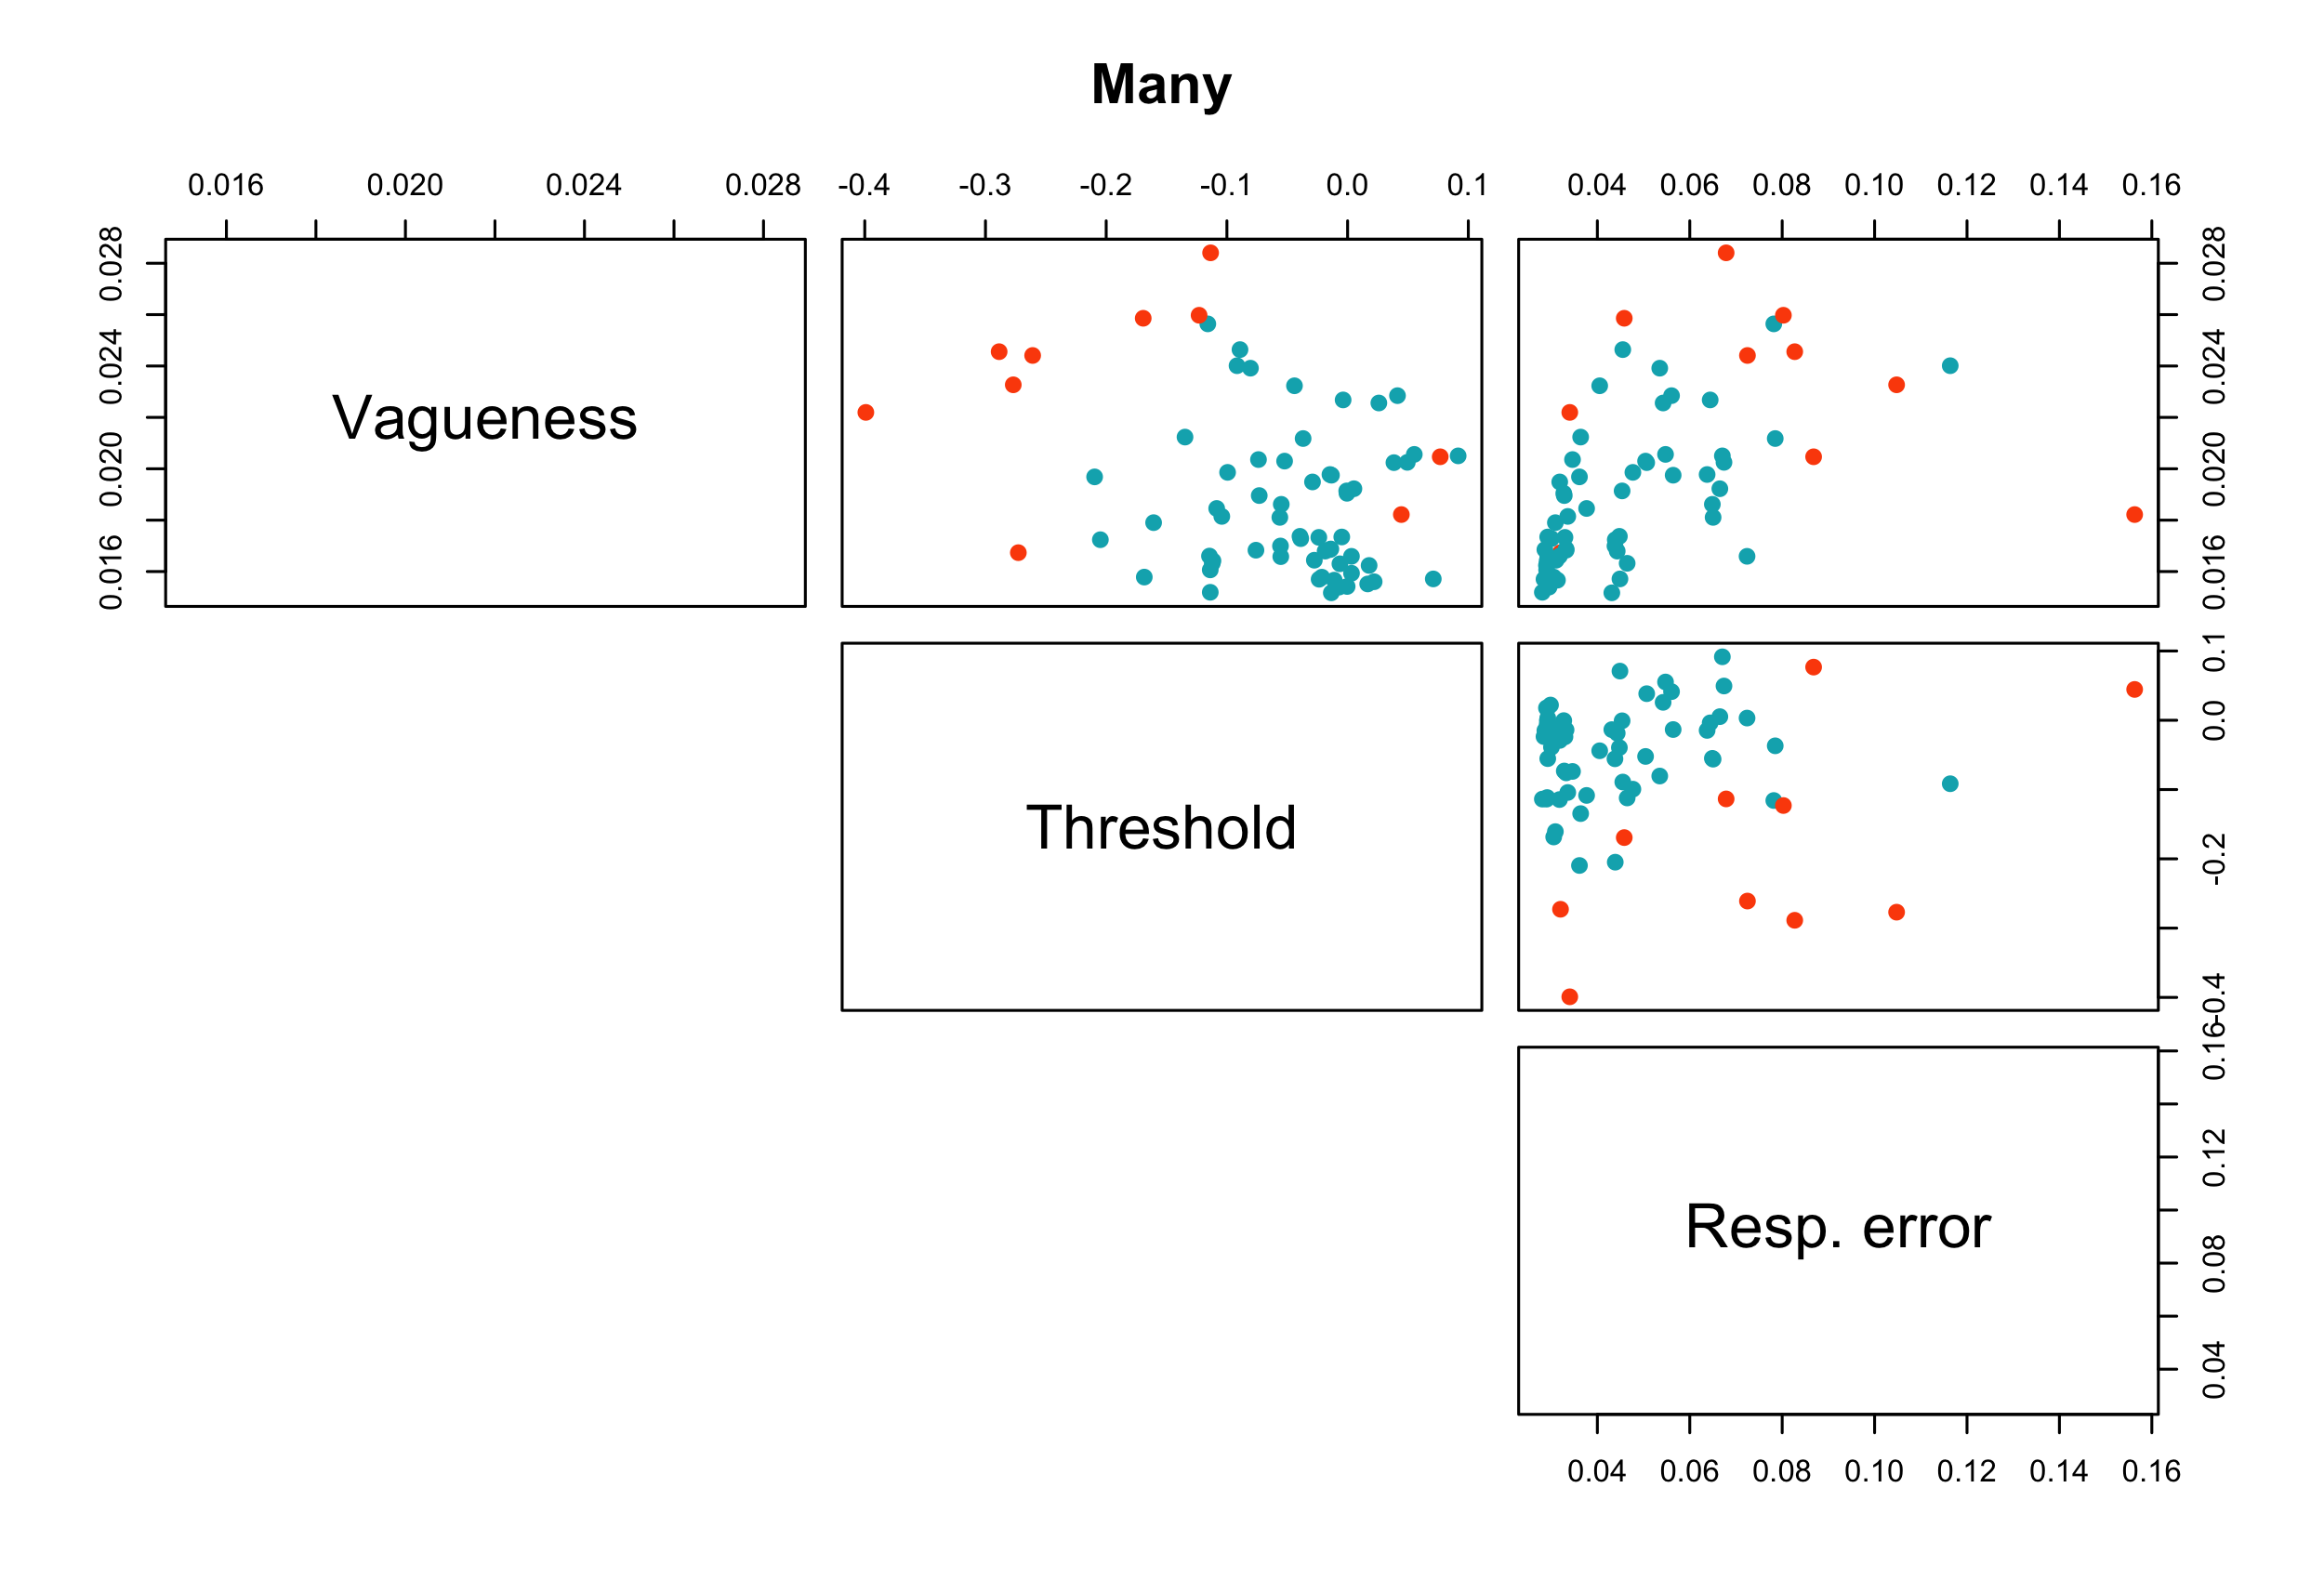
\includegraphics[width=\linewidth]{Figure2.11c.png}
     \caption{\label{fig:fig2.11c}}
    \end{subfigure}
   \end{minipage}
     \hfill
  \begin{minipage}[b]{0.49\textwidth} 
    \begin{subfigure}[b]{\linewidth}
     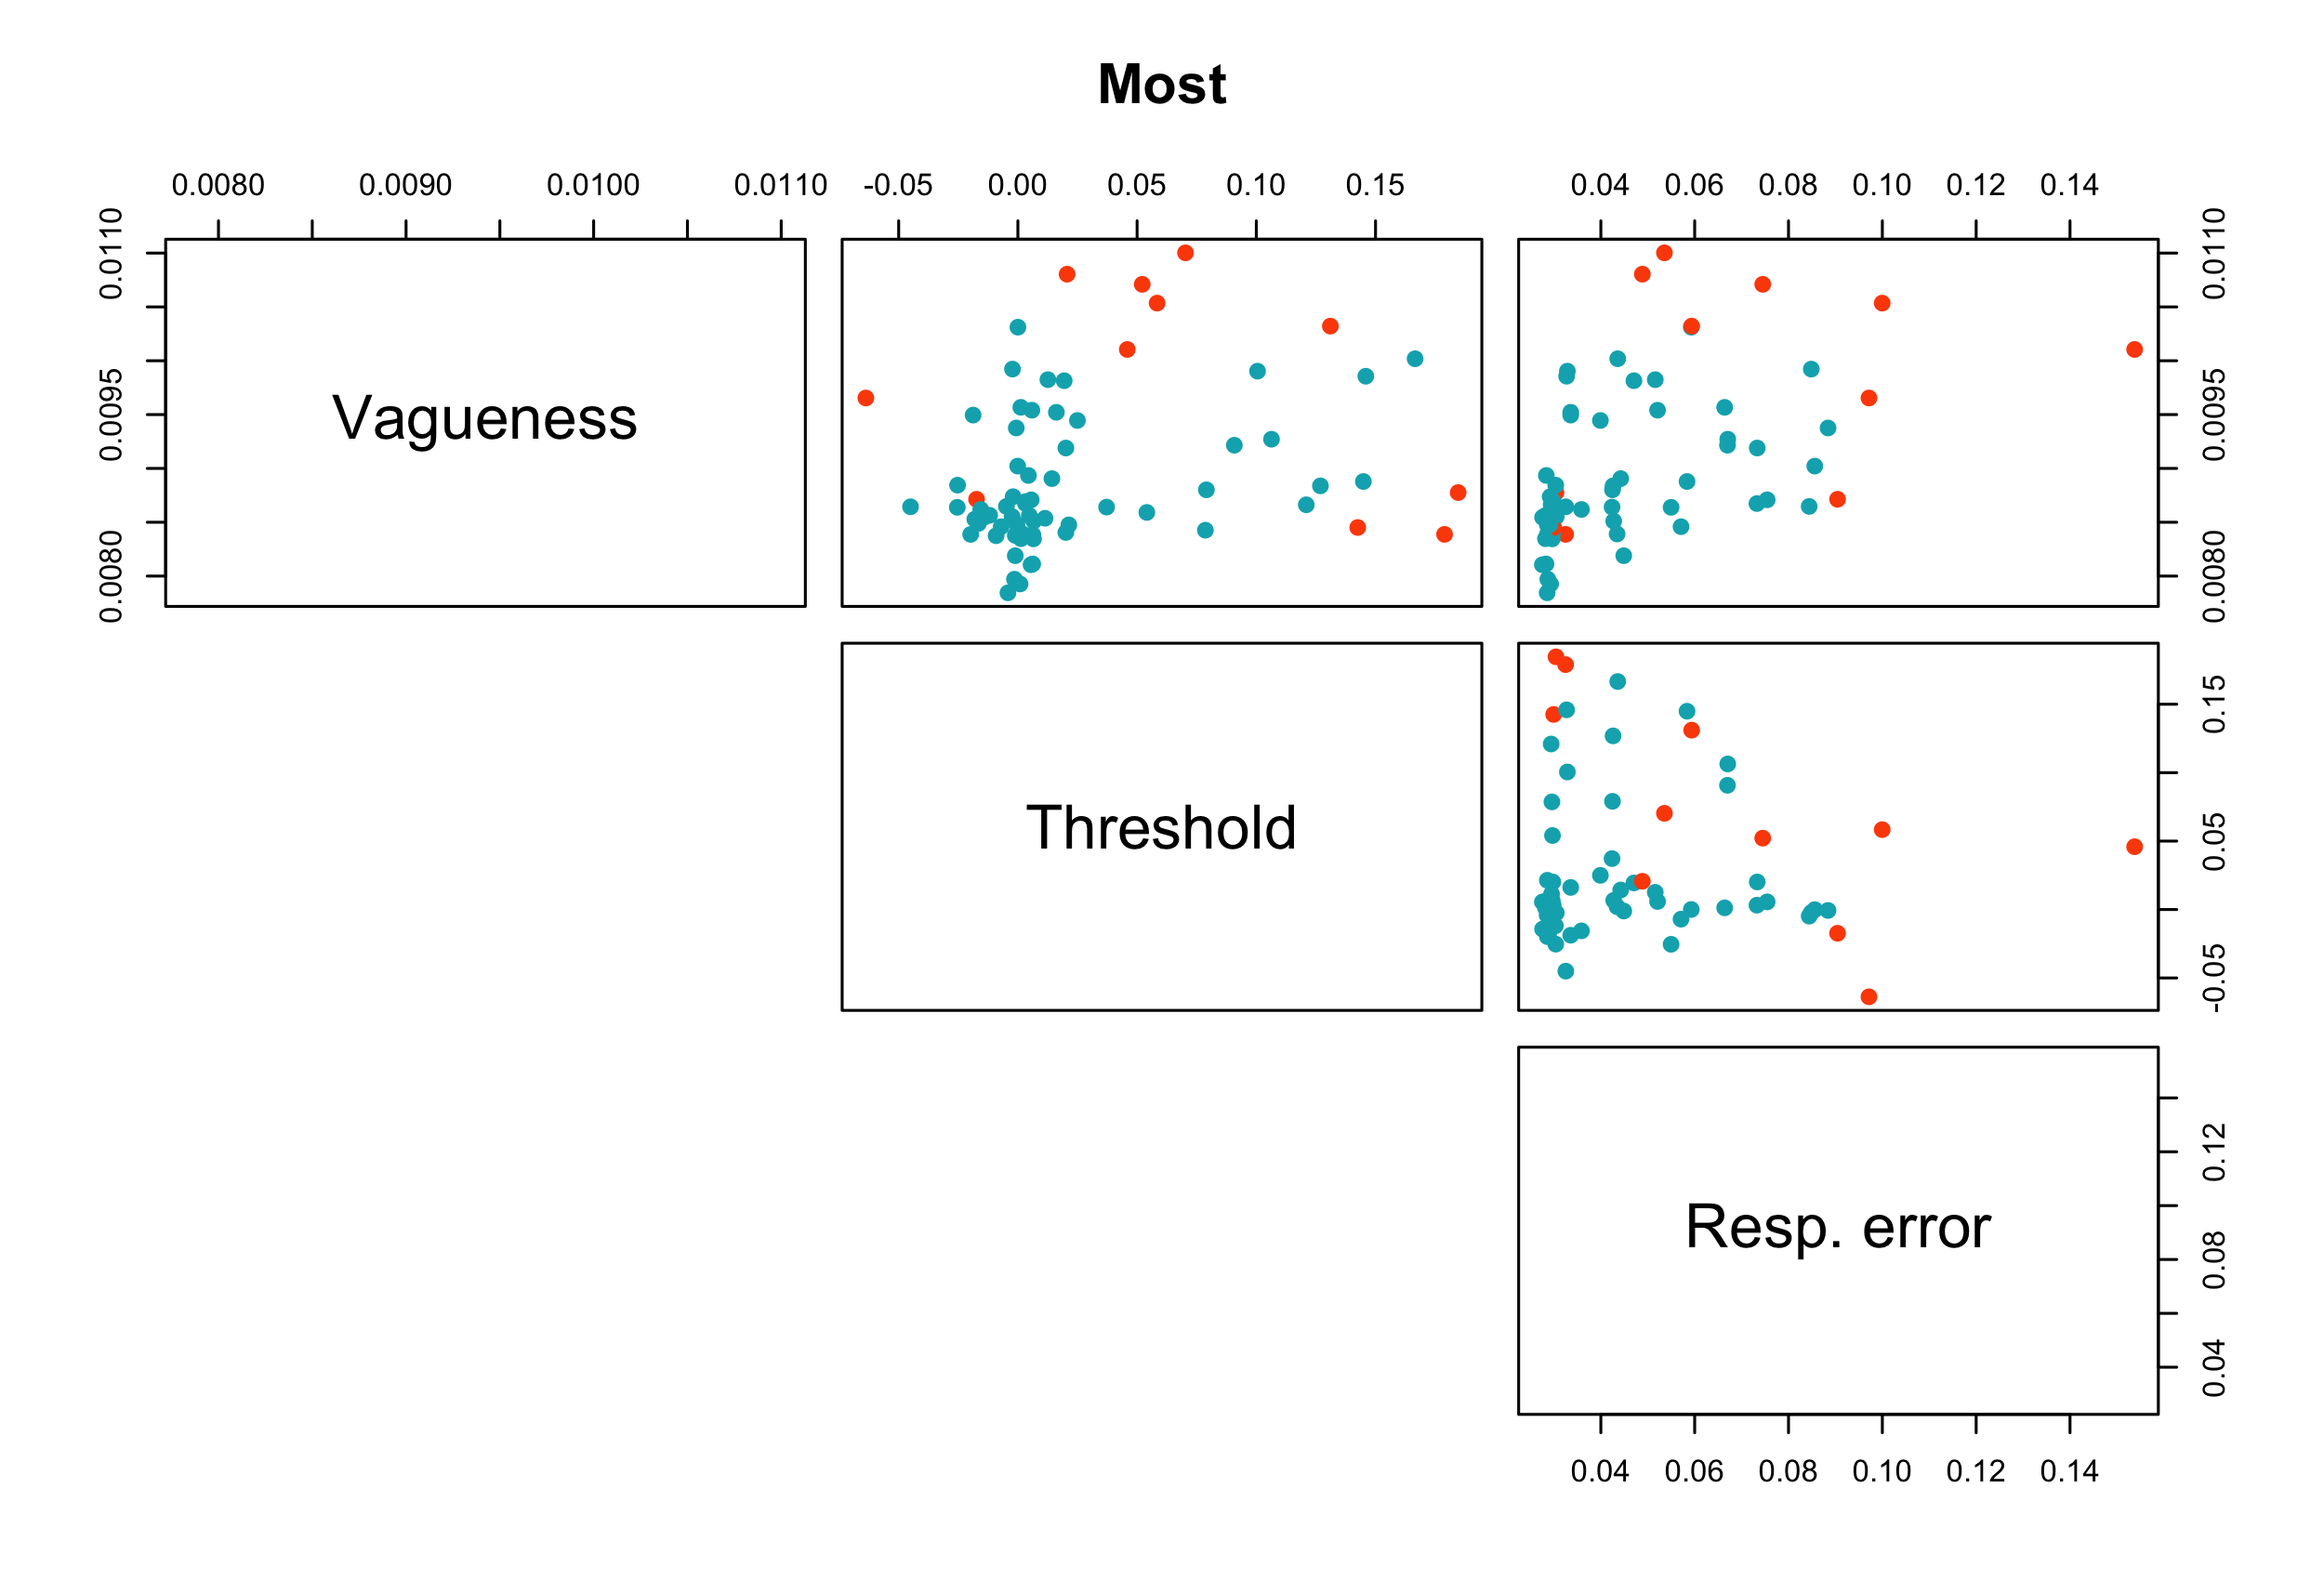
\includegraphics[width=\linewidth]{Figure2.11d.png}
     \caption{\label{fig:fig2.11d}}
    \end{subfigure}

    \vspace*{4mm}
    \begin{subfigure}[b]{\linewidth}
     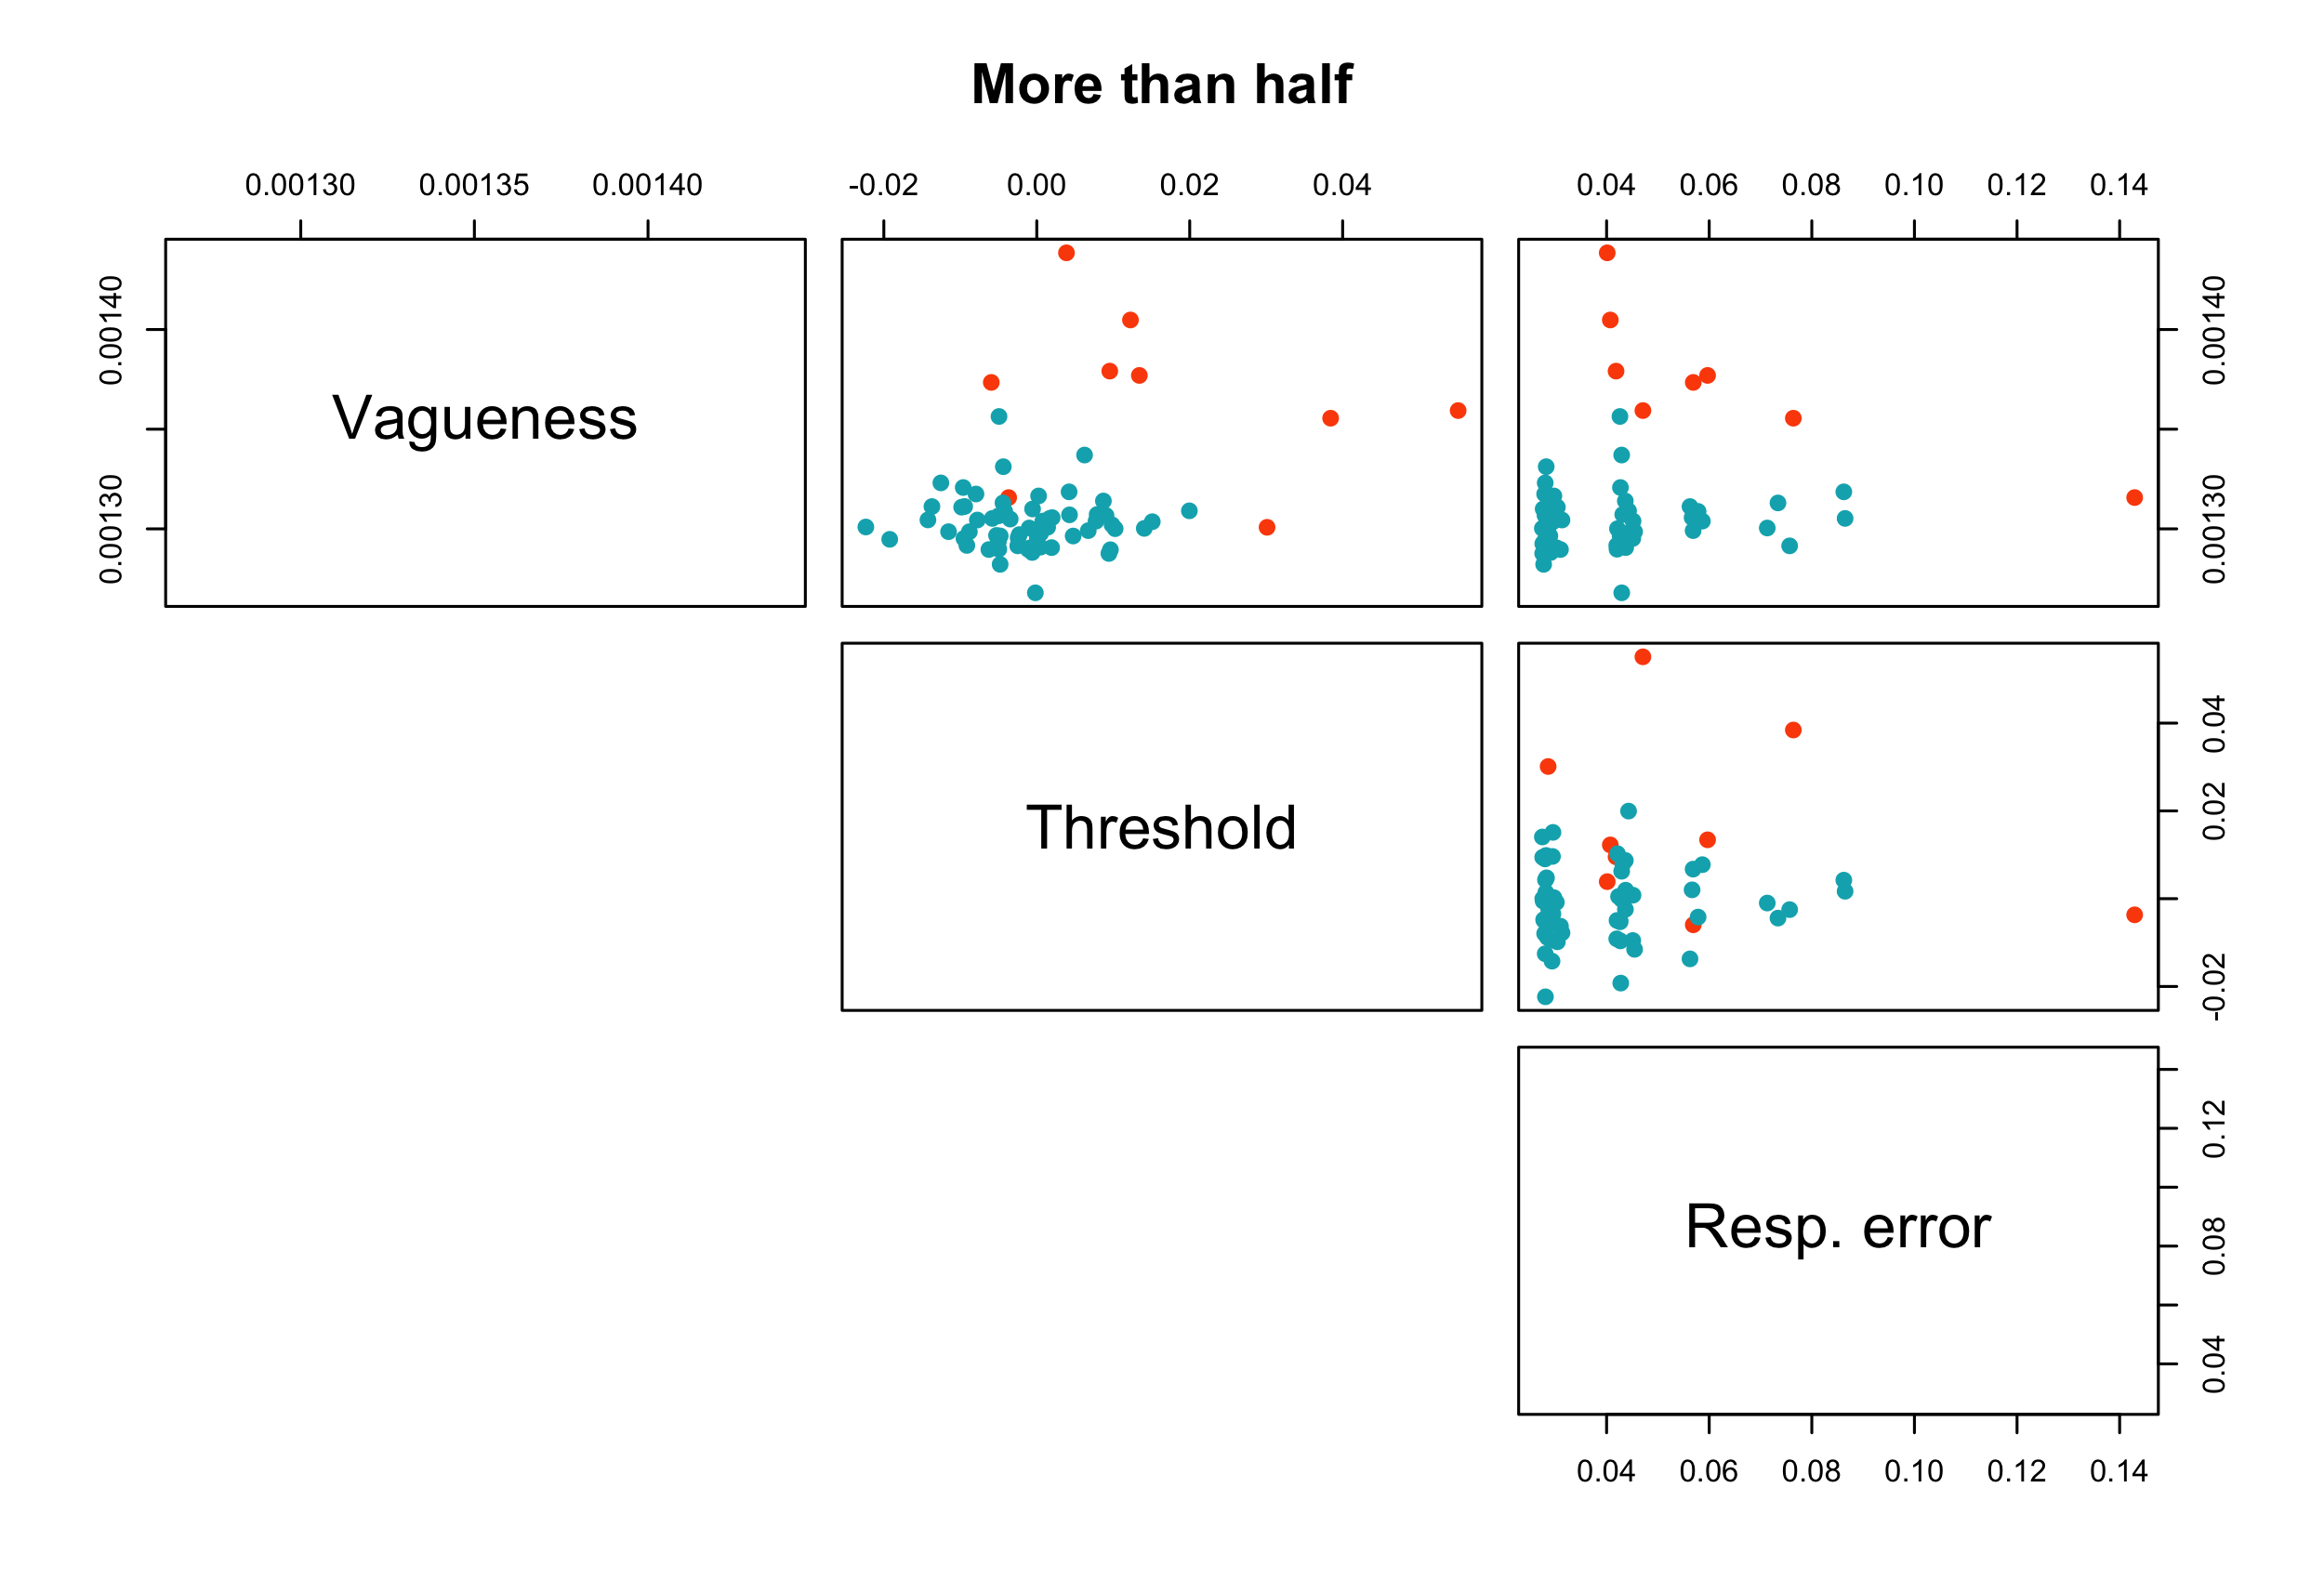
\includegraphics[width=\linewidth]{Figure2.11e.png}
     \caption{\label{fig:fig2.11e}}
    \end{subfigure}
    \end{minipage}
    
    \caption{The scatter plots illustrate the relationships between model parameters (abbreviation Resp. error - response error) for each quantifier. The influential observations according to Cook’s distance are indicated in red.}
    \label{fig:fig2.11}
\end{figure}

\end{document}
